%%%%%%%%%%%%%%%%%%%%%%%%%%%%%%%%%%%%%%%%%%%%%%%%%%%%%%%%%%%%%%%%%
%      This is thesis.tex.  You have to  put this file in       % 
%              the same directory with your thesis files.       %
%                Written by M. Imran 2001/06/18                 % 
%                 No Copyright for this file                    % 
%                 Save your time and enjoy it                   % 
%                                                               % 
%%%%%%%%%%%%%%%%%%%%%%%%%%%%%%%%%%%%%%%%%%%%%%%%%%%%%%%%%%%%%%%%%
\documentclass{dmathesis}
%% uncomment the following line to print equation labels next to
%% equation numbers. 
%\usepackage{showlabel}

%% Table of content spacing
\usepackage{setspace}

\usepackage{subcaption}

%% To place figures where you want to
\usepackage{float}

%% To remove whitespace before enumerate
\usepackage{enumitem}

%% Python code
%\usepackage{fontspec}
\usepackage{listings}

%% The following is to control the format of your thesis
%%%%%%%%%%%%%%%%%%%%%%%%%%%%%%%%%%%%%%%%%%%%%%%%%%%%%%%%%%%%%%%%%%%%%%%%%%
%     This is format.tex file needed for the dmathesis.cls file.  You    %
%  have to  put this file in the same directory with your thesis files.  %
%                Written by M. Imran 2001/06/18                          % 
%                 No Copyright for this file                             % 
%                 Save your time and enjoy it                            % 
%                                                                        % 
%%%%%%%%%%%%%%%%%%%%%%%%%%%%%%%%%%%%%%%%%%%%%%%%%%%%%%%%%%%%%%%%%%%%%%%%%%
%%%%%  Put packages you want to use here and 'fancyhdr' is required   %%%%
%%%%%%%%%%%%%%%%%%%%%%%%%%%%%%%%%%%%%%%%%%%%%%%%%%%%%%%%%%%%%%%%%%%%%%%%%%
\usepackage{fancyhdr}
\usepackage{epsfig}
\usepackage{cite}
\usepackage{graphicx}
\usepackage{amsmath}
\usepackage{theorem}
\usepackage{amssymb}
\usepackage{latexsym}
\usepackage{epic}
%%%%%%%%%%%%%%%%%%%%%%%%%%%%%%%%%%%%%%%%%%%%%%%%%%%%%%%%%%%%%%%%%%%%%%%%%%
%%%%%                 Set line spacing = 1.5 here                   %%%%%%
%%%%%%%%%%%%%%%%%%%%%%%%%%%%%%%%%%%%%%%%%%%%%%%%%%%%%%%%%%%%%%%%%%%%%%%%%%
\renewcommand{\baselinestretch}{1.5}
%%%%%%%%%%%%%%%%%%%%%%%%%%%%%%%%%%%%%%%%%%%%%%%%%%%%%%%%%%%%%%%%%%%%%%%%%%
%%%%%                      Your fancy heading                       %%%%%%
%%%%% For the final copy you need to remove '\bfseries\today' below %%%%%%
%%%%%%%%%%%%%%%%%%%%%%%%%%%%%%%%%%%%%%%%%%%%%%%%%%%%%%%%%%%%%%%%%%%%%%%%%%
\pagestyle{fancy}
%\renewcommand{\chaptermark}[1]{\markboth{\chaptername\ \thechapter.\ #1}}
%\renewcommand{\sectionmark}[1]{\markright{\thesection.\ #1}{}}
\lhead[\fancyplain{}{}]%
      {\fancyplain{}{\leftmark}}
\chead[\fancyplain{}{}]%
      {\fancyplain{}{}}
\rhead[\fancyplain{}{}]%
      {\fancyplain{}{}} %\bfseries\thepage
\lfoot[\fancyplain{}{}]%
      {\fancyplain{}{}}
\cfoot[\fancyplain{}{}]%
      {\fancyplain{}{\thepage}}
\rfoot[\fancyplain{}{}]%
      {\fancyplain{}{}} %\bfseries\today

%%%%%%%%%%%%%%%%%%%%%%%%%%%%%%%%%%%%%%%%%%%%%%%%%%%%%%%%%%%%%%%%%%%%%%%%%%
%%%%%%%%%%%%Here you set the space between the main text%%%%%%%%%%%%%%%%%%
%%%%%%%%%%%%%%%%%%%and the start of the footnote%%%%%%%%%%%%%%%%%%%%%%%%%%
%%%%%%%%%%%%%%%%%%%%%%%%%%%%%%%%%%%%%%%%%%%%%%%%%%%%%%%%%%%%%%%%%%%%%%%%%%
\addtolength{\skip\footins}{5mm}
%%%%%%%%%%%%%%%%%%%%%%%%%%%%%%%%%%%%%%%%%%%%%%%%%%%%%%%%%%%%%%%%%%%%%%%%%%
%%%%%      Define new counter so you can have the equation           %%%%%
%%%%%    number 4.2.1a for example, this a gift from J.F.Blowey      %%%%%
%%%%%%%%%%%%%%%%%%%%%%%%%%%%%%%%%%%%%%%%%%%%%%%%%%%%%%%%%%%%%%%%%%%%%%%%%%
\newcounter{ind}
\def\eqlabon{
\setcounter{ind}{\value{equation}}\addtocounter{ind}{1}
\setcounter{equation}{0}
\renewcommand{\theequation}{\arabic{chapter}%
         .\arabic{section}.\arabic{ind}\alph{equation}}}
\def\eqlaboff{
\renewcommand{\theequation}{\arabic{chapter}%
         .\arabic{equation}}
\setcounter{equation}{\value{ind}}}
%%%%%%%%%%%%%%%%%%%%%%%%%%%%%%%%%%%%%%%%%%%%%%%%%%%%%%%%%%%%%%%%%%%%%%%%%%
%%%%%%%%%%%%           New theorem you want to use              %%%%%%%%%%
%%%%%%%%%%%%%%%%%%%%%%%%%%%%%%%%%%%%%%%%%%%%%%%%%%%%%%%%%%%%%%%%%%%%%%%%%%
{\theorembodyfont{\rmfamily}\newtheorem{Pro}{{\textbf Proposition}}[section]}
{\theorembodyfont{\rmfamily}\newtheorem{The}{{\textbf Theorem}}[section]}
{\theorembodyfont{\rmfamily}\newtheorem{Def}[The]{{\textbf Definition}}}
{\theorembodyfont{\rmfamily}\newtheorem{Cor}[The]{{\textbf Corollary}}}
{\theorembodyfont{\rmfamily}\newtheorem{Lem}[The]{{\textbf Lemma}}}
{\theorembodyfont{\rmfamily}\newtheorem{Exp}{{\textbf Example}}[section]}
\def\remark{\textbf{Remark}:}
\def\remarks{\textbf{Remarks}:}
\def\bproof{\textbf{Proof}: }
\def\eproof{\hfill$\Box$}
%%%%%%%%%%%%%%%%%%%%%%%%%%%%%%%%%%%%%%%%%%%%%%%%%%%%%%%%%%%%%%%%%%%%%%%%%%
%%%%%%%    Bold font in math mode, a gift from J.F.Blowey       %%%%%%%%%%
%%%%%%%%%%%%%%%%%%%%%%%%%%%%%%%%%%%%%%%%%%%%%%%%%%%%%%%%%%%%%%%%%%%%%%%%%%
\def\bv#1{\mbox{\boldmath$#1$}}
%%%%%%%%%%%%%%%%%%%%%%%%%%%%%%%%%%%%%%%%%%%%%%%%%%%%%%%%%%%%%%%%%%%%%%%%%%
%%%%%%%        New symbol which is not defined in Latex         %%%%%%%%%%
%%%%%%%                 a gift from J.F.Blowey                  %%%%%%%%%%
%%%%%%%%%%%%%%%%%%%%%%%%%%%%%%%%%%%%%%%%%%%%%%%%%%%%%%%%%%%%%%%%%%%%%%%%%%
% The Mean INTegral
% to be used in displaystyle
\def\mint{\textstyle\mints\displaystyle}
% to be used in textstyle
\def\mints{\int\!\!\!\!\!\!{\rm-}\ }
%
% The Mean SUM
% to be used in displaystyle
\def\msum{\textstyle\msums\displaystyle}
% to be used in textstyle
\def\msums{\sum\!\!\!\!\!\!\!{\rm-}\ }
%%%%%%%%%%%%%%%%%%%%%%%%%%%%%%%%%%%%%%%%%%%%%%%%%%%%%%%%%%%%%%%%%%%%%%%%%%
%%%%%%%%%%            Define your short cut here              %%%%%%%%%%%%
%%%%%%%%%%%%%%%%%%%%%%%%%%%%%%%%%%%%%%%%%%%%%%%%%%%%%%%%%%%%%%%%%%%%%%%%%%
\def\poincare{Poincar\'e }
\def\holder{H\"older }





















%% File to be included while running latex.
\includeonly{chapter1,chapter2,chapter3%
                 ,chapter4,chapter5,chapter6,chapter7, chapter8, chapter9, ref,append}

\begin{document}

%% Front page of thesis
%%%%%%%%%%%%%%%%%%%%%%%%%%%%%%%%%%%%%%%%%%%%%%%%%%%%%%%%%%%%%%%%%%%%%%%%%%
%   This is frontpage.tex file needed for the dmathesis.cls file.  You   %
%  have to  put this file in the same directory with your thesis files.  %
%                Written by M. Imran 2001/06/18                          % 
%                 No Copyright for this file                             % 
%                 Save your time and enjoy it                            % 
%                                                                        % 
%%%%%%%%%%%%%%%%%%%%%%%%%%%%%%%%%%%%%%%%%%%%%%%%%%%%%%%%%%%%%%%%%%%%%%%%%%%
%%%%%%%%%%%%%%%%%%%%%%%%%%%%%%%%%%%%%%%%%%%%%%%%%%%%%%%%%%%%%%%%%%%%%%%%%%%
%%%%%%%%%%%%%%%%           The title page           %%%%%%%%%%%%%%%%%%%%%%%  
%%%%%%%%%%%%%%%%%%%%%%%%%%%%%%%%%%%%%%%%%%%%%%%%%%%%%%%%%%%%%%%%%%%%%%%%%%%
\pagenumbering{roman}
%\pagenumbering{arabic}

\setcounter{page}{1}

\newpage

\thispagestyle{empty}
\begin{center}
  \vspace*{1cm}
  {\Huge \bf Deep Sentiment Analysis on Tumblr}

  \vspace*{2cm}
  {\LARGE\bf Anthony Hu}

  \vfill
  {\large
  A dissertation submitted in partial fulfilment\\ 
  [-3mm] of the requirements for the degree of\\
  [-3mm] Master of Science in Applied Statistics\\}
  \vspace*{0.1cm}
  
  % Put your university logo here if you wish.
   \begin{center}
   
\includegraphics[width=0.25\textwidth]{Images/ox_logo.png}
   \end{center}

  {\large
          Department of Statistics\\
          [-3mm] University of Oxford\\
          [-3mm] Oxford, United Kingdom\\
          [1mm]  September 2017}

\end{center}

%%%%%%%%%%%%%%%%%%%%%%%%%%%%%%%%%%%%%%%%%%%%%%%%%%%%%%%%%%%%%%%%%%%%%%%%%%%
%%%%%%%%%%%%%%%% The dedication page, if you have one  %%%%%%%%%%%%%%%%%%%%  
%%%%%%%%%%%%%%%%%%%%%%%%%%%%%%%%%%%%%%%%%%%%%%%%%%%%%%%%%%%%%%%%%%%%%%%%%%%
%\newpage
%\thispagestyle{empty}
%\begin{center}
 %\vspace*{2cm}
  %\textit{\LARGE {Dedicated to}}\\ 
 %Someone here
%\end{center}


%%%%%%%%%%%%%%%%%%%%%%%%%%%%%%%%%%%%%%%%%%%%%%%%%%%%%%%%%%%%%%%%%%%%%%%%%%%
%%%%%%%%%%%%%%%%%%          The declaration page         %%%%%%%%%%%%%%%%%%  
%%%%%%%%%%%%%%%%%%%%%%%%%%%%%%%%%%%%%%%%%%%%%%%%%%%%%%%%%%%%%%%%%%%%%%%%%%%
\chapter*{Declaration}
\addcontentsline{toc}{chapter}{\numberline{}Declaration}
The work in this thesis is based on research carried out at the Department of Statistics, University of Oxford. No part of this thesis has been submitted elsewhere for any other degree or qualification and it is all my own work unless referenced to the contrary in the text.


\vfill
\noindent \textbf{Copyright \copyright\; 2017 by Anthony Hu}.\\
``The copyright of this thesis rests with the author.  No quotations
from it should be published without the author's prior written consent
and information derived from it should be acknowledged''.



%%%%%%%%%%%%%%%%%%%%%%%%%%%%%%%%%%%%%%%%%%%%%%%%%%%%%%%%%%%%%%%%%%%%%%%%%%%
%%%%%%%%%%%%%%%%%%     The acknowledgements page         %%%%%%%%%%%%%%%%%%  
%%%%%%%%%%%%%%%%%%%%%%%%%%%%%%%%%%%%%%%%%%%%%%%%%%%%%%%%%%%%%%%%%%%%%%%%%%%
\chapter*{Acknowledgements}
\addcontentsline{toc}{chapter}{\numberline{}Acknowledgements}
I would like to warmly thank my thesis supervisor Dr Seth Flaxman for his guidance and help. I am gratefully indebted to his valuable comments on this thesis.
I also want to express my profound gratitude to my parents for giving me the opportunity to study in Oxford, and for their unfaltering support throughout my years of study. 

%%%%%%%%%%%%%%%%%%%%%%%%%%%%%%%%%%%%%%%%%%%%%%%%%%%%%%%%%%%%%%%%%%%%%%%%%%%
%%%%%%%%%%%%%%%%%%           The abstract page         %%%%%%%%%%%%%%%%%%%%  
%%%%%%%%%%%%%%%%%%%%%%%%%%%%%%%%%%%%%%%%%%%%%%%%%%%%%%%%%%%%%%%%%%%%%%%%%%%
\newpage
\thispagestyle{plain}
\addcontentsline{toc}{chapter}{\numberline{}Abstract}
\begin{center}
  \textbf{\Large Deep Sentiment Analysis on Tumblr}

  \vspace*{1cm}
  \textbf{\large Anthony Hu}

  \vspace*{0.5cm}
  {\large Submitted for the degree of Master of Science in Applied Statistics\\ September 2017}

  \vspace*{1cm}
  \textbf{\large Abstract}
\end{center}
We propose a novel approach to Sentiment Analysis using Deep Neural Networks combining Visual Recognition and Natural Language Processing. Our approach leverages Tumblr posts containing images and text to predict the emotional state of users. Deep convolutional layers extract relevant features of the images and high-dimensional word embedding followed by a recurrent layer process the textual information to accurately infer the emotion of a given Tumblr post. We demonstrate that the network architecture, named Deep Sentiment, learns meaningful relations between visual data and language as it vastly outperforms models using a single modality. We then show that Deep Sentiment can also be adapted to generate images and text representative of an emotion. 

%%%%%%%%%%%%%%%%%%%%%%%%%%%%%%%%%%%%%%%%%%%%%%%%%%%%%%%%%%%%%%%%%%%%%%%%%%%
%%%%%%%%    tableofcontents, listoffigures and listoftables       %%%%%%%%%
%%%%%%%%        Command if you do not have  them                  %%%%%%%%%
%%%%%%%%%%%%%%%%%%%%%%%%%%%%%%%%%%%%%%%%%%%%%%%%%%%%%%%%%%%%%%%%%%%%%%%%%%%
\begin{spacing}{0.95}
\tableofcontents
\end{spacing}
\listoffigures
\listoftables
\clearpage


%%%%%%%%%%%%%%%%%%%%%%%%%%%%%%%%%%%%%%%%%%%%%%%%%%%%%%%%%%%%%%%%%%%%%%%%%%%
%%%%%%%%%%%%%%%%%%%%%%   END OF FRONT PAGE %%%%%%%%%%%%%%%%%%%%%%%%%%%%%%%%
%%%%%%%%%%%%%%%%%%%%%%%%%%%%%%%%%%%%%%%%%%%%%%%%%%%%%%%%%%%%%%%%%%%%%%%%%%%











%% Main text
% set page number starts from 1
\pagenumbering{arabic}
\setcounter{page}{1}

%% To ensure the equation counter works correctly
%\eqlabon
%\eqlaboff

\chapter{Introduction}

Sentiment analysis has been an active area of research in the past few years, especially on the readily available Twitter data, e.g. Bollen et al. \cite{bollen} who investigated the impact of collective mood states on stock market or Flaxman et al. \cite{seth-twitter} who analysed day-of-week population well-being.

Contrary to Twitter, Tumblr's posts are not limited to 140 characters, allowing more expressiveness, and are not centered on the textual content but on the image content instead. A Tumblr post will almost always be an image with some text accompanying the latter. Pictures have become prevalent on social media and characterising them could enable the understanding of billions of users. 

We propose a novel method to uncover the emotional state of an individual posting on social media. The ground truth emotion will be extracted from the tags, considered as the `self-reported' emotion of the user. Our model incorporates both text and image and we aim to `read' them to be able to understand the emotional content they imply about the user. Concretely, the Deep Sentiment model associates the features learned by the two modalities as follows:

\begin{itemize}
    \item We fine-tune a pre-trained Deep Convolutional Neural Network, named Inception \cite{googlenet}, trained on the ImageNet dataset to our specific task of emotion inferring.
    \item We project the text in a rich high-dimensional space with a word representation learned by Word2Vec \cite{word2vec}, that was trained on billions of words. The word vectors then go through a Recurrent Neural Network which preserves the word order and captures the semantics of human language.
    \item A fully-connected layer combines the information in the two modalities and a final softmax output layer gives the probability distribution of the emotional state of the user.
\end{itemize}

We will also see that Deep Sentiment can be rearranged to generate Tumblr posts expressing one of the learned emotion.










\chapter{Tumblr Data}

%%%%%%%%%%%%%%%%%%%%%%%%%%%%%%%%%%%%%%%%%%%%%%%%%%%%%%%%%%%%
%%%%%%%%%%%%%%%%%%%%  NEW SECTION   %%%%%%%%%%%%%%%%%%%%%%%%
%%%%%%%%%%%%%%%%%%%%%%%%%%%%%%%%%%%%%%%%%%%%%%%%%%%%%%%%%%%%
\section{Overview of the Data}
Tumblr posts were retrieved using the Python API, here is an example of a post:
\begin{figure}[H]
\centering
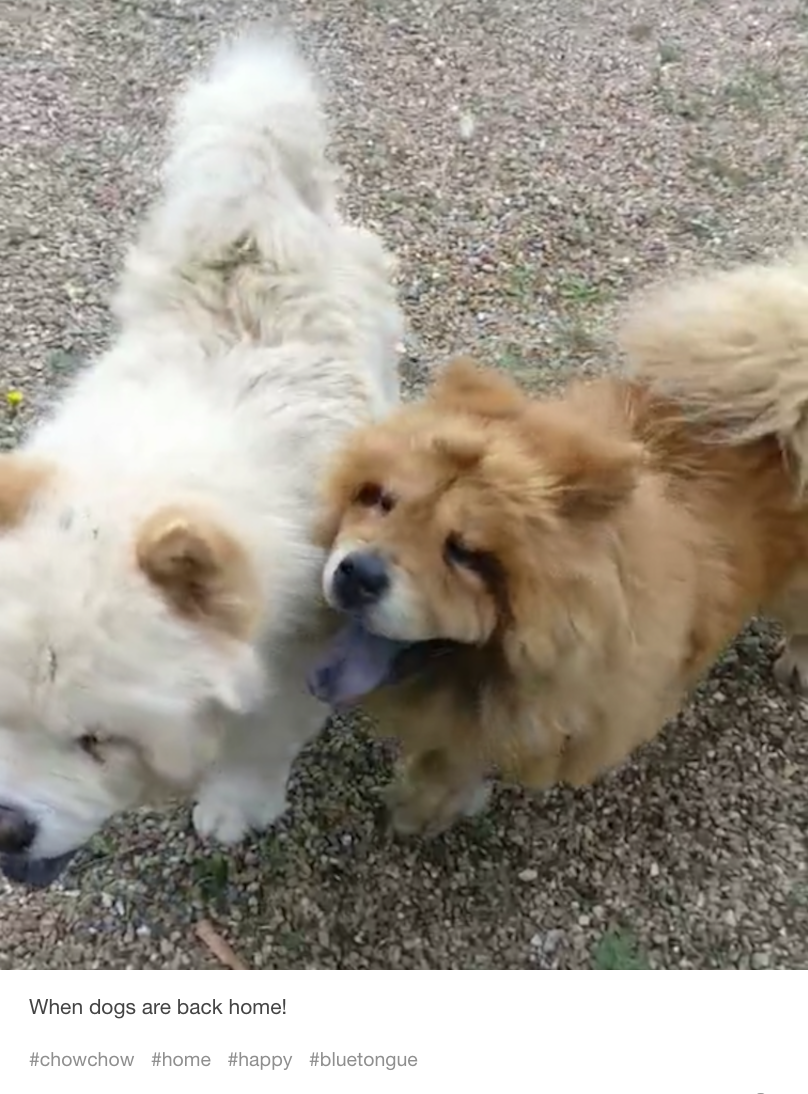
\includegraphics[width=.58\textwidth]{Images/chowchow.png}
\caption{An example of a Tumblr post}
\end{figure}

The tags `\#chowchow \# home \#happy \#bluetongue' are really valuable as they indicate the user's state of mind when writing that post. Ekman popularised the idea that there are six basic emotions \cite{ekman}: hapiness, sadness, anger, surprise, fear, disgust. These emotions are said to be {\em basic} as they are hardwired regardless of the species: basic emotions are innate, universal and automatic and induce fast reactions that are linked with a high survival rate.

To build our dataset, queries were made searching for each of the six emotions appearing in the tags. Adjectives were used as they were more commonly used by users: \#happy, \#sad, \#angry, \#surprised, \#scared and \#disgusted. Each post would then contain the following information:
\begin{enumerate}
\item The text. In the example above: \textit{When dogs are back home!}
\item The image.
\item The associated emotion: one among the six classes.
\end{enumerate}

Note that sometimes, a post would contain several basic emotions such as `\#sad \#angry'. We simply selected the first hashtag written by the user as it can be deemed as the main emotion that the user first thought of.

The data extraction took several weeks due to the API's limitations: 1,000 requests per hour and 5,000 requests per day, with each request containing 20 posts. The dataset contains about 1 million posts.

\section{Data Preprocessing}
In some posts, the tag also appeared in the text itself, for instance:
\begin{quote}
\textit{``When you're on vacations and there is a rainstorm. \#fail \#sad"}.
\end{quote}
Keeping the \textit{\#sad} would bias the learning process and the neural network would simply learn to detect the presence or absence of that tag. To ensure that the network is actually learning something, we removed from the text the hashtags containing the emotion to be predicted.

Also, Tumblr is used worldwide, therefore posts not written in English had to be removed from the training data. Basically, if a post contains less than a given number of English word, it is deemed as non-English and removed from the dataset. The threshold was set to 5 English words as it appears to filter out reasonably well the dataset. The vocabulary of English words was obtained from Word2Vec and will be detailed further in Section 4.

Figure \ref{fig:emotions} shows examples of posts with their associated emotions:

\begin{figure}
\begin{subfigure}[t]{.5\textwidth}
  \vskip 0pt %Necessary to align on image and not caption
  \centering
  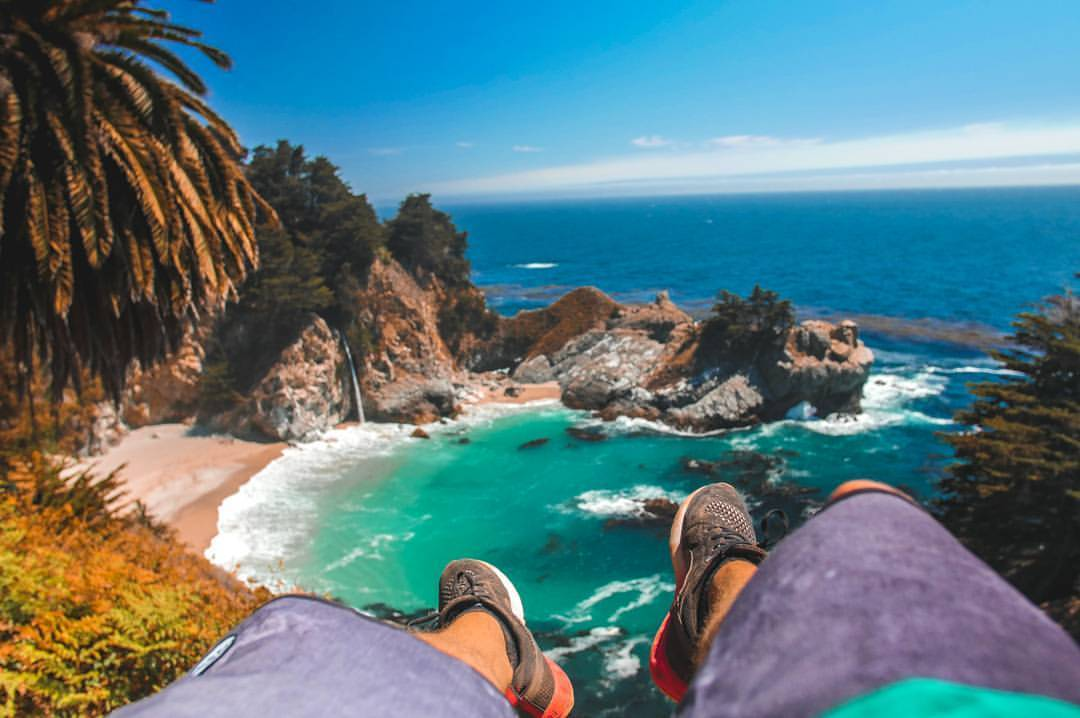
\includegraphics[width=.8\linewidth]{Images/happy.jpg}
  \caption{\textbf{Happy}: ``Just relax with this amazing view \#bigsur \#california \#roadtrip \#usa \#life \#fitness (at McWay Falls)"}
\end{subfigure}
\begin{subfigure}[t]{.5\textwidth}
  \vskip 0pt 
  \centering
  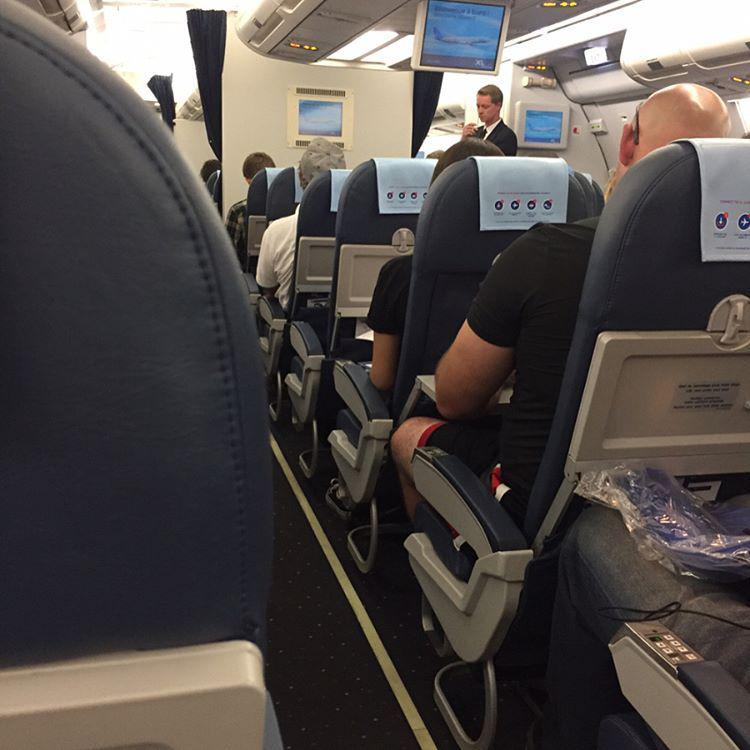
\includegraphics[width=.7\linewidth]{Images/scared.jpg}
  \caption{\textbf{Scared}: ``On a plane guys! We're about to head out into the sky to Paris, France \#Paris \#trip \#kinda \#nervous \#fun \#vacations"}
\end{subfigure}
\begin{subfigure}[t]{.5\textwidth}
  \vskip 0pt
  \centering
  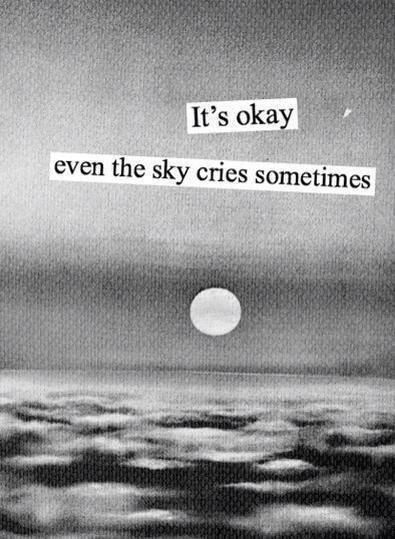
\includegraphics[width=.6\linewidth]{Images/sad.jpg}
  \caption{\textbf{Sad}: ``It's okay to be upset. It's okay to not always be happy. It's okay to cry. Never hide your emotions in fear of upsetting others or of being a bother   If you think no one will listen. Then I will."}
\end{subfigure}
\begin{subfigure}[t]{.5\textwidth}
  \vskip 0pt 
  \centering
  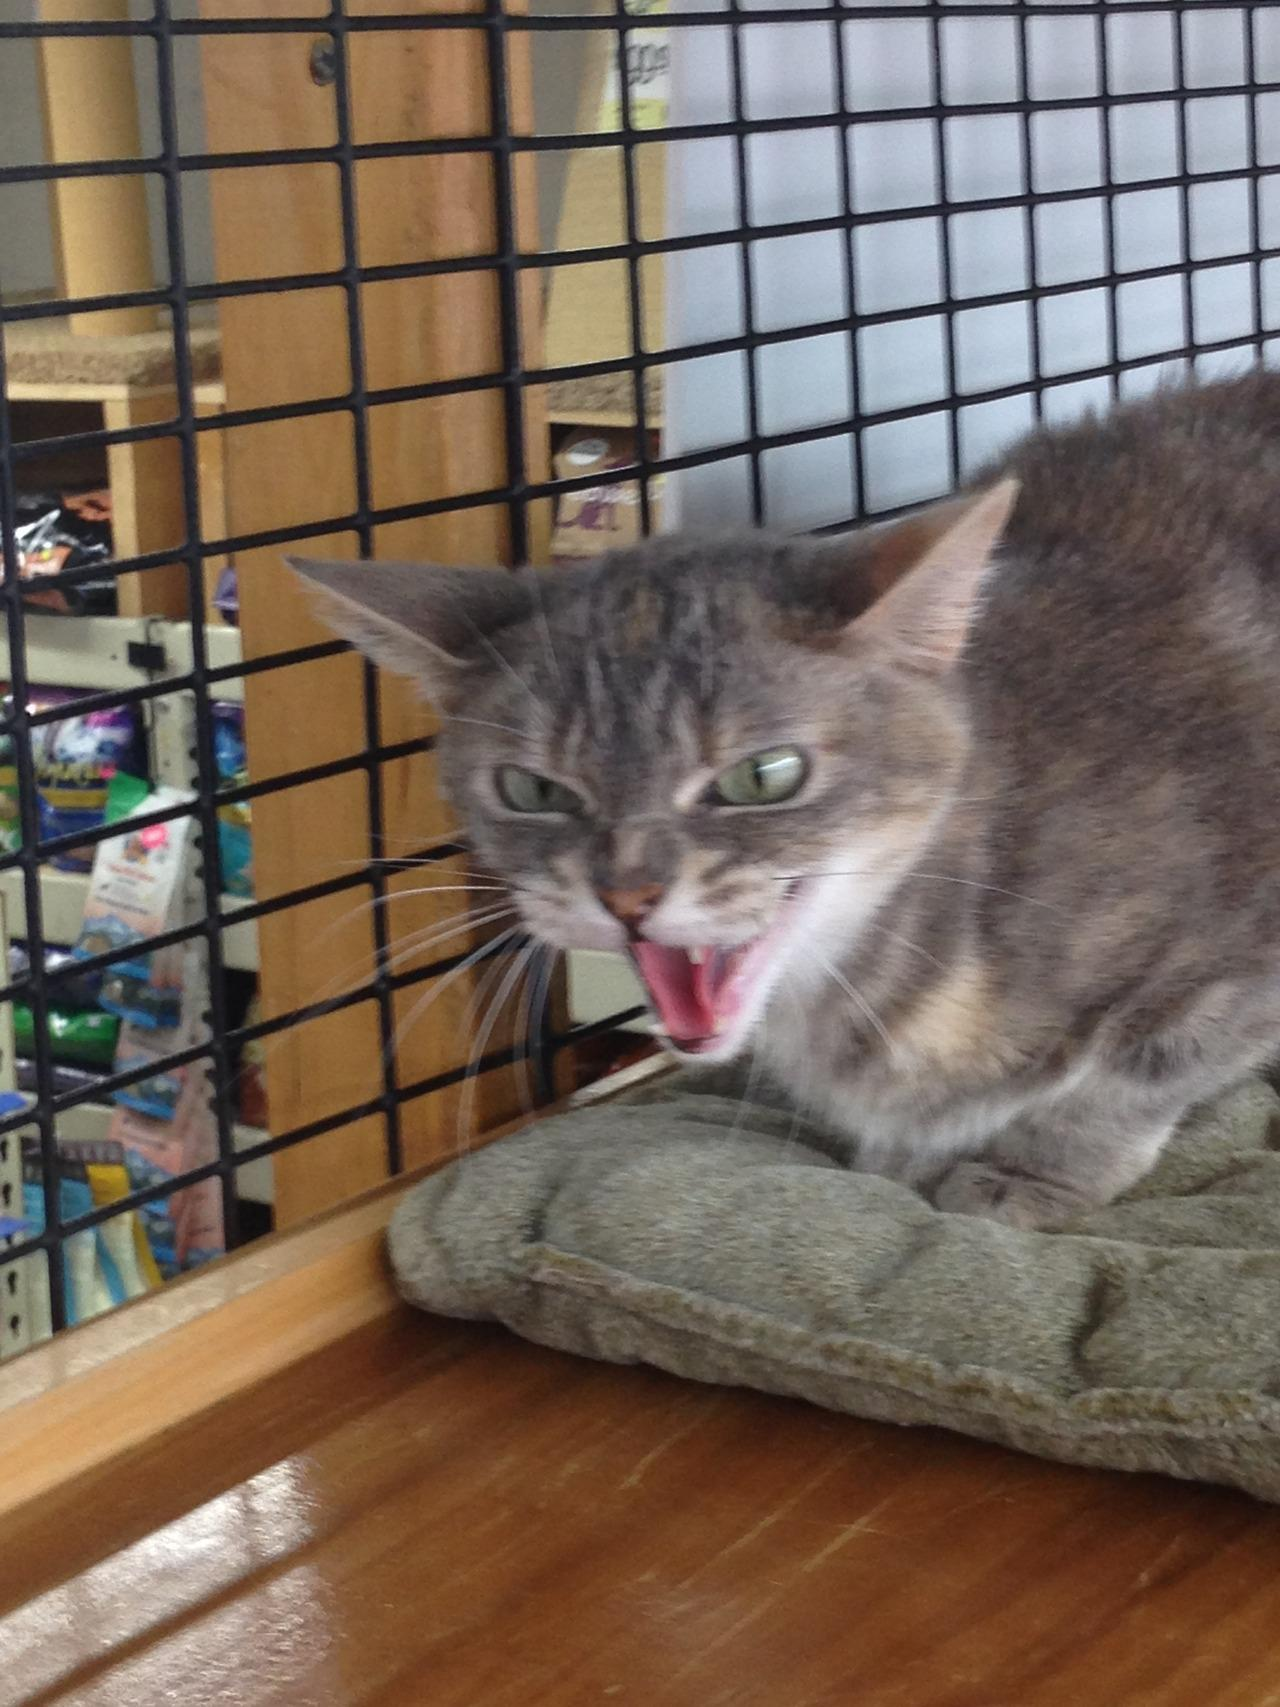
\includegraphics[width=.5\linewidth]{Images/angry.jpg}
  \caption{\textbf{Angry}: ``Tensions were high this Caturday..."}
\end{subfigure}
\begin{subfigure}[t]{.5\textwidth}
  \vskip 0pt 
  \centering
  
\includegraphics[width=.8\linewidth]{Images/surprised.jpg}
  \caption{\textbf{Surprised}: ``Which Tea? Peppermint tea: What is your favorite gif right now?"}
\end{subfigure}
\begin{subfigure}[t]{.5\textwidth}
  \vskip 0pt 
  \centering
  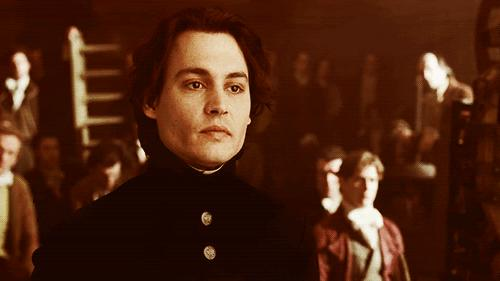
\includegraphics[width=.8\linewidth]{Images/disgusted.jpg}
  \caption{\textbf{Disgusted}: ``Me when I see a couple expressing their affection in physical ways in public"}
\end{subfigure}
\caption{The 6 emotions illustrated by Tumblr posts \cite{tumblr-photos}}
\label{fig:emotions}
\end{figure}
\chapter{Visual recognition}
The pictures are valuable to accurately determine the emotion of the user. For instance, happy photos might contain sunny landscapes and sandy beaches while sad pictures might contain darker colors. To analyse the images, we'll use convolutional neural networks, which achieve state-of-the-art performances in many visual recognition tasks. First we'll explain how they work and then we'll dive into the architecture we've used for deep sentiment analysis.
%%%%%%%%%%%%%%%%%%%%%%%%%%%%%%%%%%%%%%%%%%%%%%%%%%%%%%%%%%%%
%%%%%%%%%%%%%%%%%%%%  NEW SECTION   %%%%%%%%%%%%%%%%%%%%%%%%
%%%%%%%%%%%%%%%%%%%%%%%%%%%%%%%%%%%%%%%%%%%%%%%%%%%%%%%%%%%%
\section{Convolutional neural networks}
A convolutional neural networks, often called ConvNets, can be seen as a simulation of the human visual cortex, that is to say an aggregation of plenty of receptive fields. (some illustrations might be helpful here)

\subsection{Convolutional layer}
Take an image of dimension $(h,w,3)$ with $h$ the height, $w$ the width and 3 representing the number of channels (red, blue, green). If you simply flatten that image and transform it into a vector of size $h\times h \times 3$ and feed that vector to a neural network, you'll get average results as you've thrown away all the spatial information. Convolutions extract that spatial information and work the following way:
\begin{itemize}
\item Each convolution is described by a filter F of size $(f, f, 3)$, $f$ usually being equal to 3, 5, or 7.
\item Position the filter on the upper left of the image and element-wise multiply with the filter, then sum those numbers to obtain a `neuron'.
\item Slide across the image, one pixel at a time horizontally and vertically, and repeat the previous operation (see Figure \ref{convolution}).
\end{itemize}

\begin{figure}
\begin{subfigure}[t]{.5\textwidth}
  \vskip 0pt
  \centering
  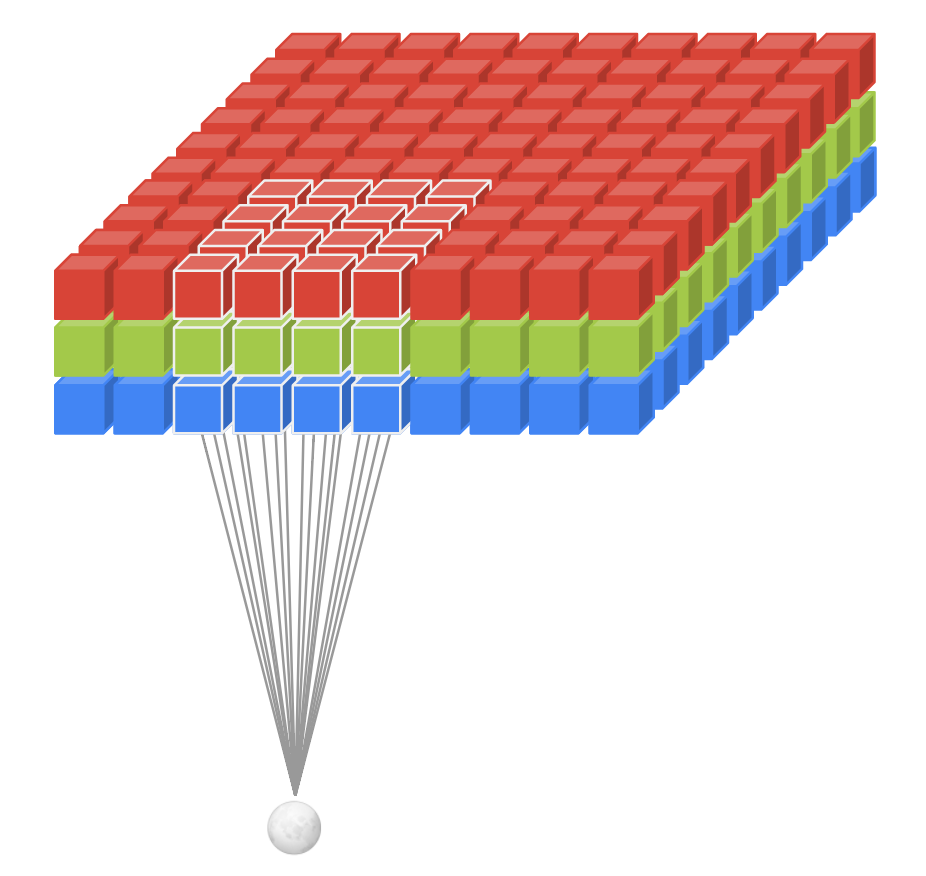
\includegraphics[width=.8\linewidth]{Images/conv1.png}
  \caption{One operation of convolution}
\end{subfigure}
\begin{subfigure}[t]{.5\textwidth}
  \vskip 0pt 
  \centering
  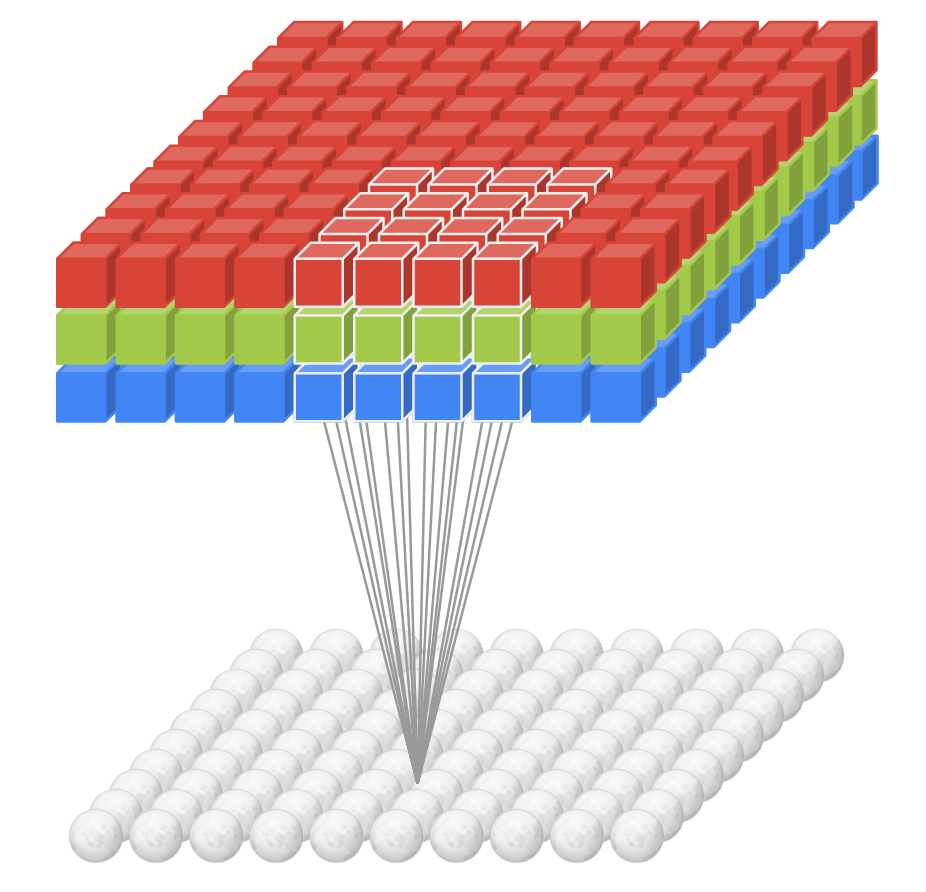
\includegraphics[width=.8\linewidth]{Images/conv2.png}
  \caption{The result of the convolution}
\end{subfigure}
\caption{A convolution, each neuron been a `receptive field' \cite{gorner}}
\label{convolution}
\end{figure}

By sliding through the image, you will get a new matrix of dimension $(h_{new}, w_{new},1)$, with $h_{new}=h-f+1$ and $w_{new}=w-f+1$. However, we usually don't want to reduce the size of our input image that fast, as we want to stack several convolutions. To ensure that the image has the same size after each convolution, zero-padding is used: we add $p$ zeros to the borders of the input image to preserve the spatial size of the input. (illustration needed, before and after zero-padding)With zero-padding, $h_{new}$ becomes: $h_{new} =  h + 2p - f + 1$, and we want that $h_{new}$ to be equal to $h$:
\begin{equation}
h + 2p - f + 1 = h
\end{equation}
Therefore, $p=\frac{f-1}{2}$. Besides, zeros are used instead of any other number because you want the filter to activate on the pixels of the image only, therefore, setting the added border to zeros ensure that the resulting neuron will not be influenced by the border.

A convolution extracts information about the image such as edges or blotches of some color (Figure \ref{conv-ex}). The grayscale and edges filters were hardcoded but in a ConvNet setting, the weights of the filter F are learned through optimising a loss function -- in our case, a metric measuring how accurate our predictions of the emotions are. The network will learn weights that will detect features that will be most relevant to our specific task. A convolution also has a depth parameter $d$: simply repeat the operation described above $d$ times with $d$ independent filters of the same size $(f, f, 3)$, to create a new tensor of dimension $(h,w,d)$.

We can then apply convolutions on that new tensor. First layers will detect simple features such as edges or aggregation of colors, and deeper layers might recognise more complex features such as faces or wheels.

\begin{figure}
\centering
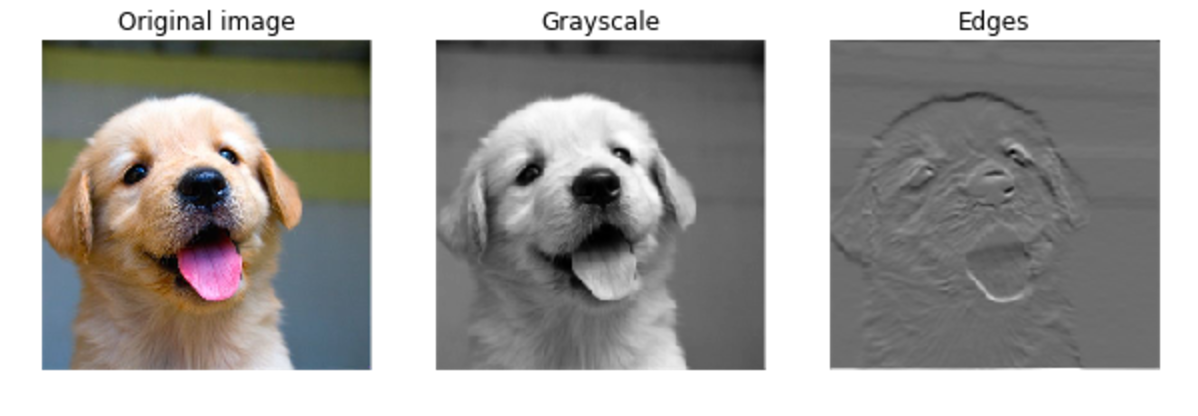
\includegraphics[width=0.8\textwidth]{Images/conv_ex.png}
\caption{Examples of convolution}
\label{conv-ex}
\end{figure}

\subsection{ReLU layer}
Stacking convolutions is nice, but as it is, we are only creature features that are linearly dependent of the input pixels: we could in fact replace all the convolutions with a single matrix multiplication. In order to learn more interesting functions, we have to add non-linearities. Historically, the popular choice was the sigmoid function defined as:
\begin{equation}
\text{sigmoid}(x) = \frac{1}{1+e^{-x}}
\end{equation}

\begin{figure}[H]
\centering
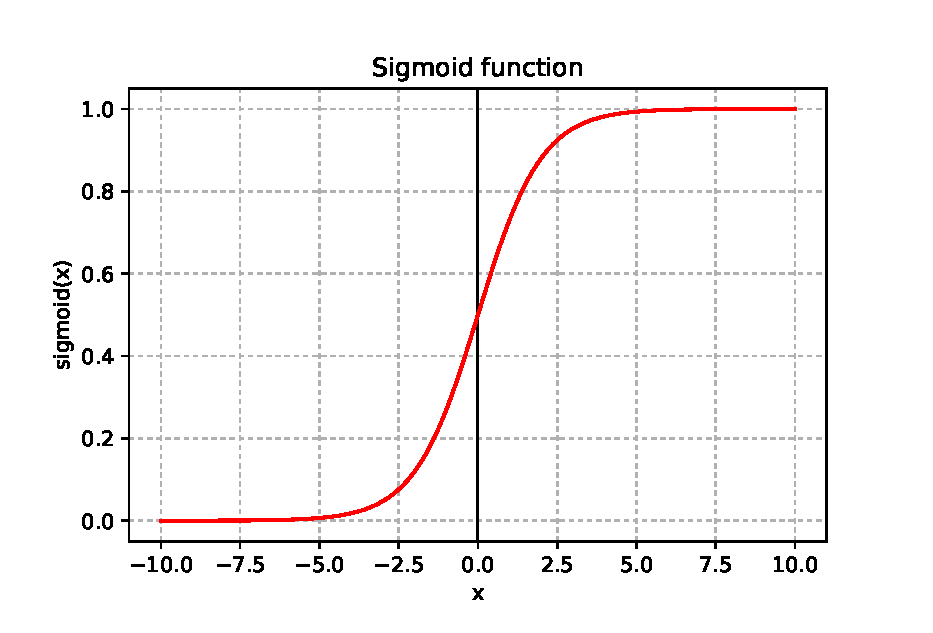
\includegraphics[width=0.5\textwidth]{Images/sigmoid.eps}
\caption{Sigmoid function}
\end{figure}

The sigmoid function is the simplest function having values between 0 and 1 mimicking the biological neurons `firing' in reaction to their inputs. However, when the network is learning to minimise a loss function through backpropagation, the gradients tend to vanish to zero as the sigmoid's derivative goes to zero for high negative and positive values. The most popular choice of non-linearity is now the Rectified Linear Unit (ReLU) defined as:
\begin{equation}
\text{ReLU}(x) = \text{max}(0,x)
\end{equation}

\begin{figure}[H]
\centering
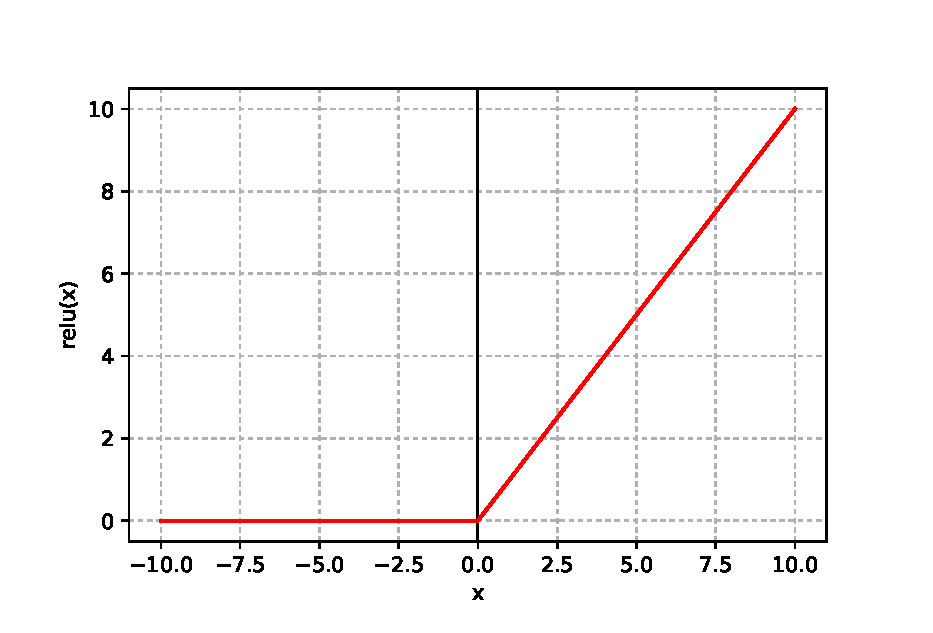
\includegraphics[width=0.5\textwidth]{Images/relu.eps}
\caption{ReLU function}
\end{figure}

The ReLU's gradient is non-saturating for highly excited neurons which turns out to be a nice property to learn faster. In the network, each layer of convolution is followed by a ReLU layer, that simply applies the function $\text{max}(0,x)$ to each neuron.

\newpage
\subsection{Pooling layer}
There is a lot of spatial redundancy in an image, we don't need all the pixels to be able to identify what's in a picture. For example we can perfectly identify the animal in Figure \ref{kittens} by reducing the number of pixels by two.

\begin{figure}[H]
\centering
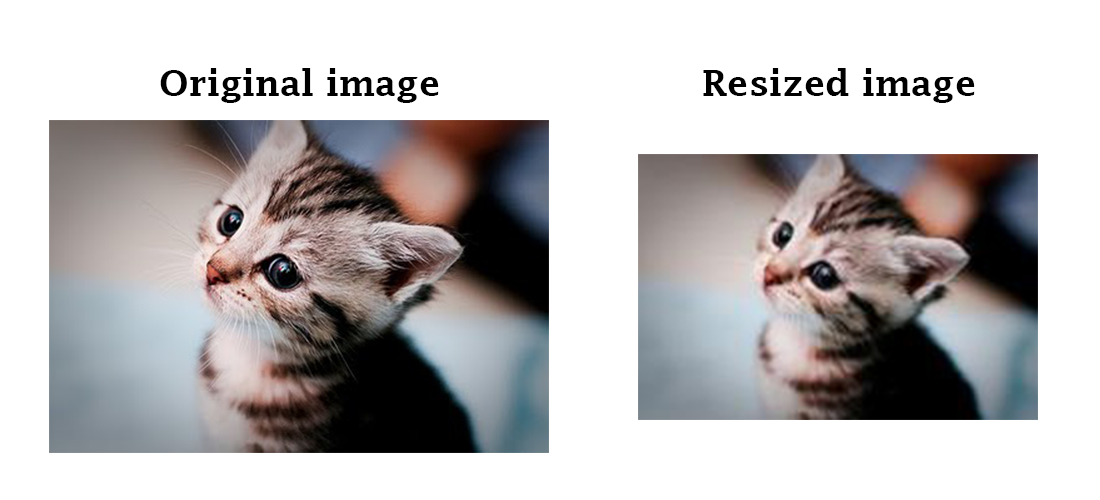
\includegraphics[width=0.8\textwidth]{Images/kittens.png}
\caption{A kitten, and the same kitten with half the pixels}
\label{kittens}
\end{figure}

The same idea applies to convolved images, we might not need all the neurons that were created. The pooling operation downsamples the image in the following way:
\begin{itemize}
\item Pick a channel among the $d$ ones.
\item Position yourself on the top-left 2x2 square of the image and take the max.
\item Repeat by sliding through the image vertically and horizontally with a stride/step of 2 (see Figure \ref{maxpool}).
\end{itemize}

\begin{figure}[H]
\centering
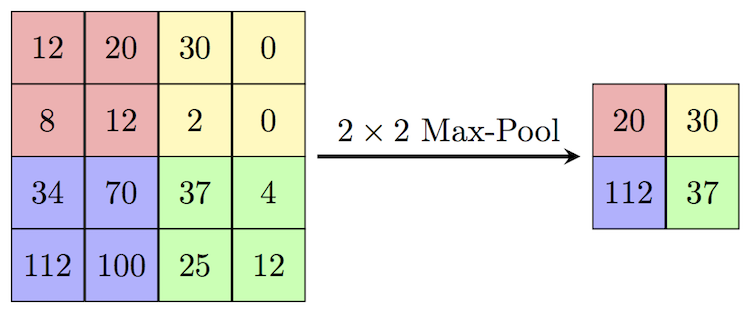
\includegraphics[width=0.8\textwidth]{Images/maxpool.png}
\caption{Max pooling \cite{camb-spark}}
\label{maxpool}
\end{figure}

After applying max pooling to each channel, the resulting image dimension is $(\frac{h}{2}, \frac{w}{2}, d)$ and we have discarded 75\% of the neurons (as in each max-pool operation, we only keep the maximum neuron among the fours), effectively reducing the number of parameters and controlling overfitting.

You could wonder why max-pooling and not average pooling (taking the mean value of the four neurons)? The convolutions allow us to see if a certain feature is in the image when a neuron fires, and we only want to know if that feature is there in a certain region. Therefore taking the max of the four neurons is sufficient to know whether that feature is there or not in that particular region.

In practice, after a few iterations of convolutions, inserting pooling layers in-between convolutional layers might be a good idea to control the spatial complexity of the network.

\subsection{An example of convolutional network}
Here is an example of a convolutional neural network with an input image of size $(224, 224, 3)$:

\begin{figure}[H]
\centering
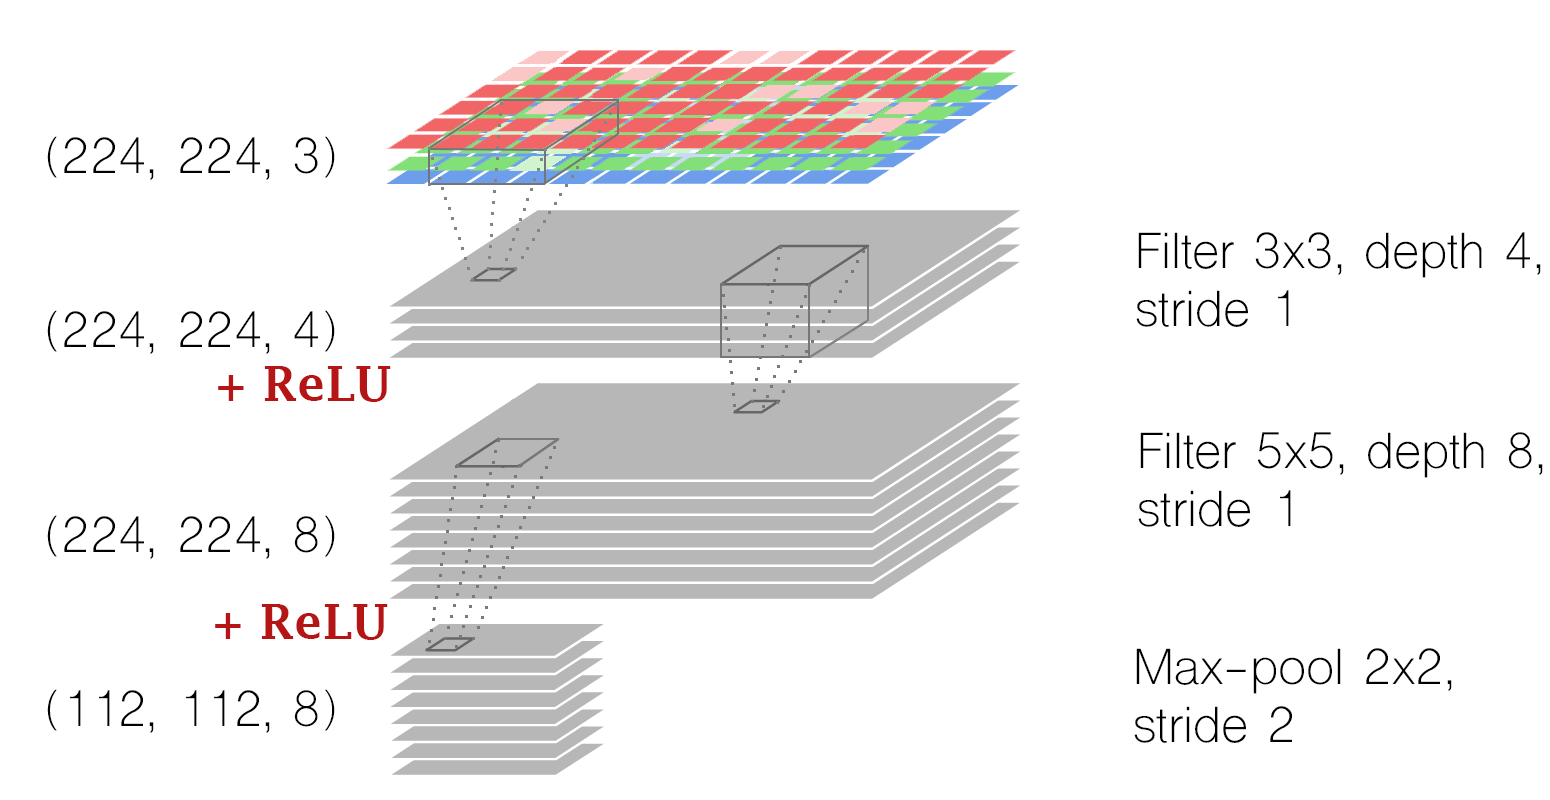
\includegraphics[width=0.8\textwidth]{Images/conv_archi.png}
\caption{An architecture of a neural network \cite{gorner}}
\end{figure}

\begin{itemize}
\item A first convolution with a filter of size $3\times3$ is applied, with depth 4, stride 1 and zero-padding of 1.
\item A ReLU layer.
\item A second convolution with a filter of size $5\times5$ is applied, with depth 8, stride 1 and zero-padding of 2.
\item A ReLU layer.
\item Max-pooling of size $2\times2$ with stride 2, reducing the height and width by 2.
\end{itemize}

After the last operation, the neurons are reshaped into a vector that can be fed to the traditional fully connected layers of neural networks.

\subsection{Deep convolutional networks}
Best results are achieved using deep convolutional networks, that is to say by stacking many layers of convolutions/ReLU/max-pool. But what exactly is `many'? Let us have a look at the main Computer Vision competition: ImageNet Large Scale Visual Recognition (ILSVR).
\begin{enumerate}
\item \textbf{AlexNet} \cite{alexnet}: The first popular convolutional network, developed by Alex Krizhevsky, Ilya Sutskever and Geoffrey Hinton, that outperformed the other competitors at ILSVR 2012 by a large margin: top-5 error of 16\% compared to the runner-up with 26\%. AlexNet has 5 convolutional layers (followed by ReLU), 3 max-pool layers and 3 fully-connected layers, producing a 8-layer deep network (not counting the max-pooling as it doesn't have any parameters).
\item \textbf{GoogLeNet} (also known as Inception)\cite{googlenet}: This is the winner of ILSVR 2014 with a top-5 error of 6.7\% . This 22-layer architecture used the `Inception Module' which allowed to drastically reduce the number of parameters: from 60M for AlexNet to 4M for GoogLeNet.
\item \textbf{ResNet} \cite{resnet}: The winner of ILSVR 2015 with a top-5 error of 3.6\% thanks to an astonishing 152 layers convolutional network. This architecture features `skip connections' allowing this ultra-deep network achieve such results.

(explain Inception module, talk about computational considerations (Stanford CS231n))
\end{enumerate}

\subsection{Transfer Learning}
Training a convolutional network from scratch can be difficult as a large amount of data is needed and plenty of different architectures and hyperparameters need to be tried before finding a decent model. To circumvent that issue, you can take advantage of the pre-trained models available that learned to recognize images through near 1.2M training examples and a deep architecture that took weeks to train on multiple GPUs.

More specifically, the pre-trained networks learned to recognise features on a picture that allow it to classify the latter among the 1000 classes there are on the ImageNet dataset. Those features are combined in the final fully connected layer to make a decision. Suppose that instead of classifying an image into 1000 classes we want to label it according to 6 different emotions (happy, sad, angry, scared, surprised, disgusted). The same features can be combined in a different way to let the network take a decision on the emotion label of the image.

The process described above is called {\em Transfer Learning}: you chop off the last layer of the network and add your own layer given how many classes you have. You then freeze the weights of the other layers and only backpropagate through the newly created layer when training the network on your examples. If you have enough data, you can unfreeze more higher-level layers and backpropagate through them. One way to see why this works is that earlier features of ConvNets contain more generic features (such as edges or color blobs), while later features become more specific to the details of the classes present in the dataset. For example in ImageNet, there are many dog breeds and the later representational power might be used to distinguish those \cite{transfer}.

We will be using Google's Inception network and fine-tune the last fully-connected layer. [an illustration would be nice].



\chapter{Natural Language Processing}
Even as a human being, it can be difficult to guess the expressed emotion by only looking at the Tumblr Image without reading the text as shown by Figure \ref{disgusted-unclear}

\begin{figure}[H]
    \centering
    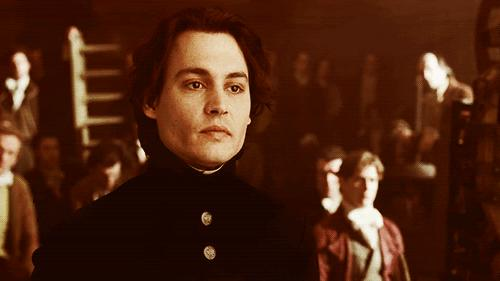
\includegraphics[width=0.5\textwidth]{Images/disgusted.jpg}
    \caption{Which emotion is it?}
    \label{disgusted-unclear}
\end{figure}

It's unclear whether the user is sad or disgusted. Only by reading the text ``Me when I see a couple expressing their affection in physical ways in public", you can finally conclude that the emotion conveyed is: {\em disgusted}. The text is extremely informative and is usually crucial to accurately infer the emotion. Neural networks only work with numbers, therefore the text has to be converted into raw numbers. A very successful way to capture the meaning of a sentence is by using word embedding.
\newpage
%%%%%%%%%%%%%%%%%%%%%%%%%%%%%%%%%%%%%%%%%%%%%%%%%%%%%%%%%%%%
%%%%%%%%%%%%%%%%%%%%  NEW SECTION   %%%%%%%%%%%%%%%%%%%%%%%%
%%%%%%%%%%%%%%%%%%%%%%%%%%%%%%%%%%%%%%%%%%%%%%%%%%%%%%%%%%%%
\section{Word Embedding}
One way to map text into numbers would be to use a dictionary that maps each word in the vocabulary (containing all the words of every Tumblr posts) to an integer. Then, you could transform any word into an one-hot vector, a vector of size the number of words in the vocabulary, with a 1 in the position of the word and 0s elsewhere. A sentence could then be encoded as a sum of vectors, that can be normalised by some distance ($L^2$ for instance). A major drawback is that this will cause data sparsity as the vocabulary size can be huge. For example, the number of 5-word sentences with a vocabulary size of 1000, is $1000^5=10^{15}$. This problem is specific to text as image and audio processing systems train on rich high-dimensional data (pixel intensities for images and spectral densities for audio), as shown by Figure \ref{comparison-text}.

\begin{figure}[H]
    \centering
    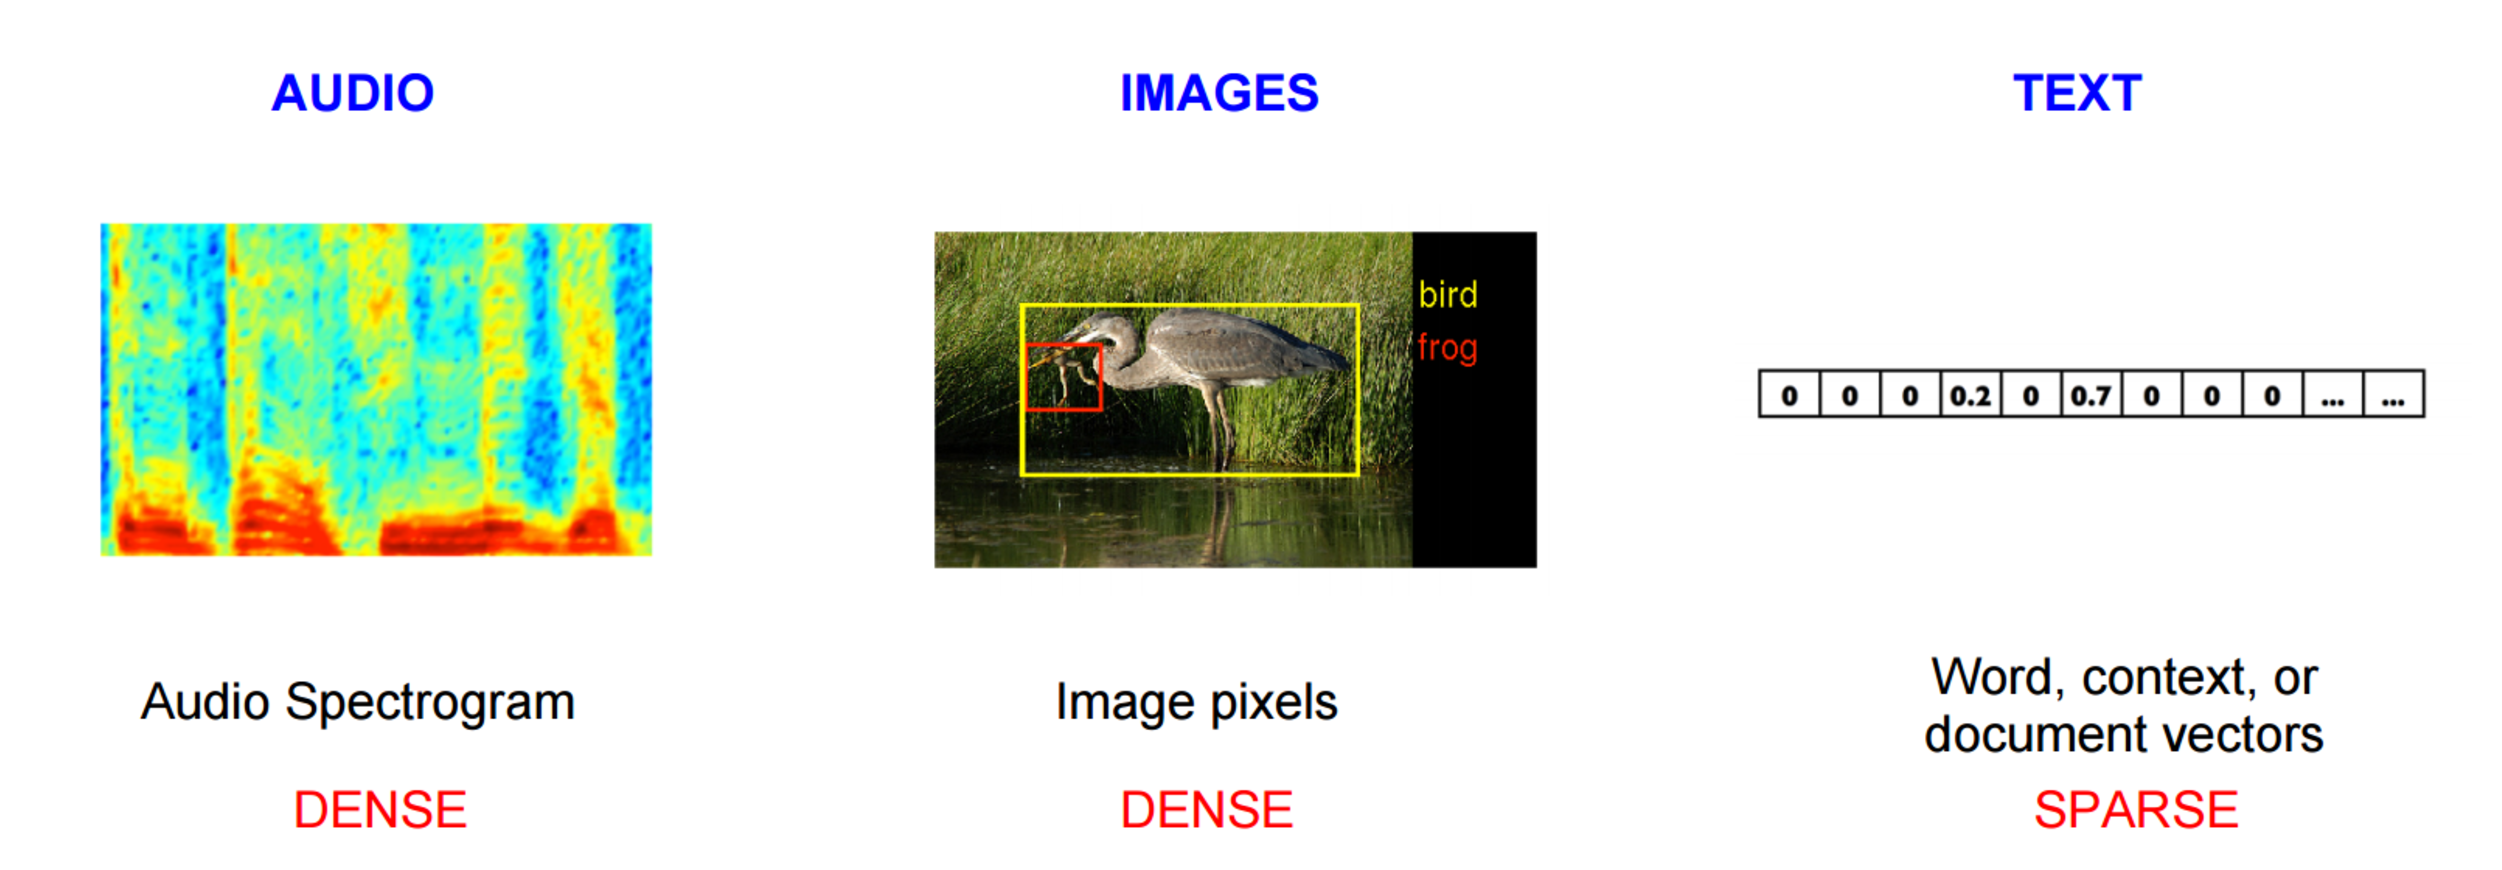
\includegraphics[width=\textwidth]{Images/comparison-text.png}
    \caption{Data sparsity in text \cite{comparison-text}}
    \label{comparison-text}
\end{figure}

Most learning algorithms rely on the local smoothness hypothesis, that is, similar training instances are spatially close. This hypothesis clearly doesn't hold with one-hot encoding as `dog' is as close to `tree' as it is to `cat'. Ideally, you would like to transform the word `dog' in a space so that it's closer to `cat' than it is to `tree'. That's exactly how word embedding works: every word is projected into a highly dimensional space that keep semantic relationships. Therefore, what the model has learned about dogs can be used when faced with a cat.

\subsection{Word2Vec Overview}
The Word2Vec model by Mikolov et al. \cite{word2vec} is an efficient implementation of word embedding and works as follow:
Suppose you have a sentence: ``the ants in the garden". We can break that sentence in (context, target) pairs where the context are the words surrounding the target word. For example, if we take a context with a window of 1, we get the following pairs: ([the, in], ants), ([ants, the], in), ([in, garden], the) [we omitted the pairs where the context wasn't of size 2]. We will then train a model to predict the target word given the context, and the weights of the model will give the word embedding (this will become clearer shortly). This model is called the Continuous Bag-of-Words model, and Word2Vec also comes in another flavor called the Skip-Gram model.

In the Skip-Gram model, we will predict the context given the target word, creating more pairs as for instance ([the, in], ants) are split into two training instances: (ants, the), (ants, in). The Continuous Bag-of-Words model smooth over the distributional information by using the whole context, and works well on smaller datasets, but by breaking the (context, target) pair into more observations, the Skip-Gram model tends to perform better on larger datasets, and that's the model we will stick on from now on.

\subsection{Skip-Gram Model}
The model is a neural network with one hidden layer and its objective is to predict the context word given the target. The input of the network will be a target word represented as a one-hot vector, of size say 10,000 (that's the vocabulary size) and the output will also be a vector of size 10,000 giving the probability distribution of the context word. Here is the architecture of the model:

\begin{figure}[H]
    \centering
    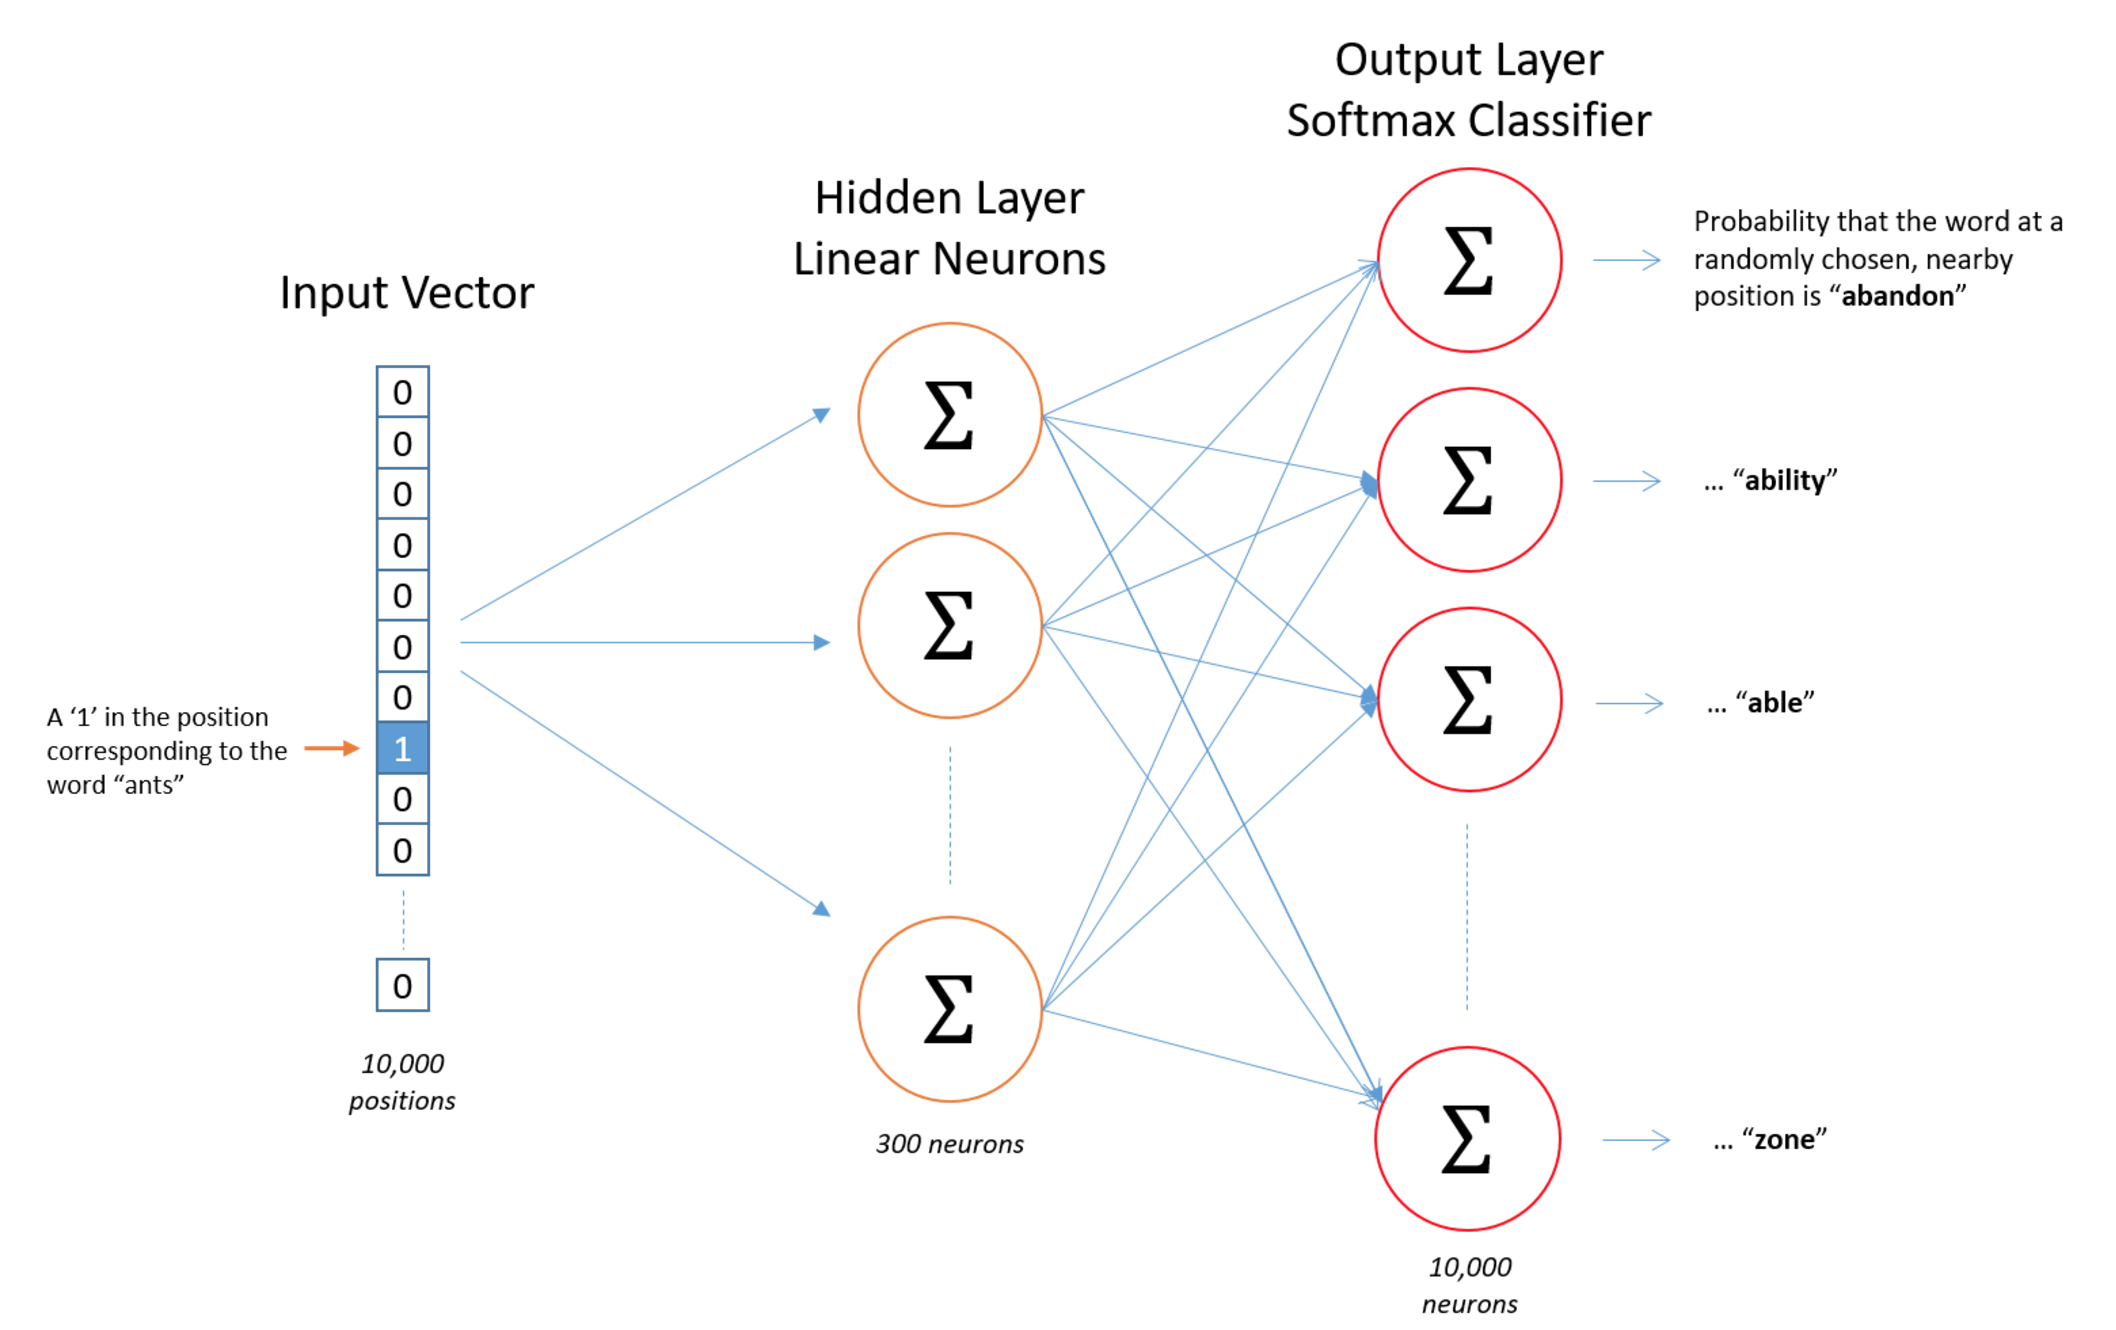
\includegraphics[width=\textwidth]{Images/word2vec-architecture.png}
    \caption{Skip-Gram model architecture \cite{word2vec-architecture}}
\end{figure}

There is no activation function in the hidden layer, but output neurons use softmax. The weights of the hidden layer matrix give the embedding as when you multiply a $1\times$10 000 one-hot vector with a 10 000$\times300$ matrix you select the row of size $1\times300$ corresponding to the high-dimensional representation of that word: 

\begin{figure}[H]
    \centering
    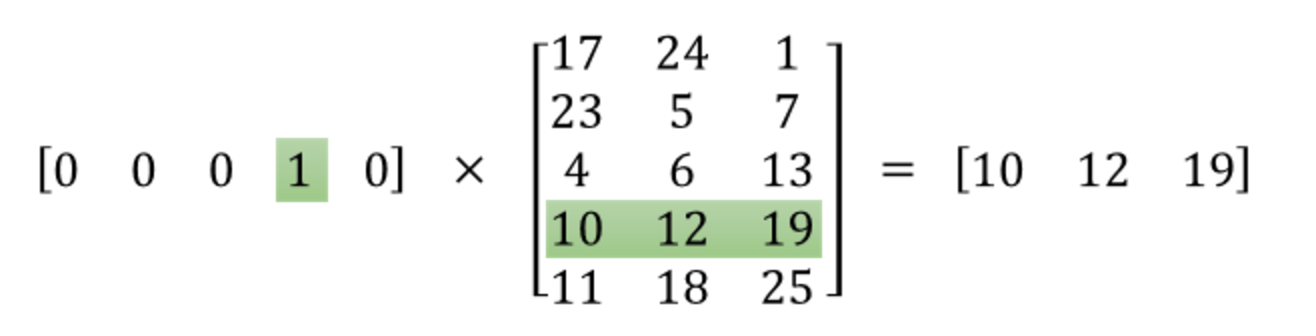
\includegraphics[width=0.8\textwidth]{Images/onehot-matrix.png}
    \caption{Where the embedding comes from \cite{word2vec-architecture}}
\end{figure}

To learn those weights, the network is minimising the cross-entropy loss given a (target word, context word) = $(w_t, w_c)$:
\begin{align}
    \text{J}_{\text{CE}}   &=  -\text{log}~P(w_c | w_t) \nonumber\\
    &= -\text{log}~\{\text{softmax}(w_c, w_t)\}\nonumber\\
    &= -\text{log}\left(\frac{\text{exp}\{\text{score}(w_c, w_t)\}}{\sum_{\text{Word w' in Vocab}}\text{exp}\{\text{score}(w_c, w')\}} \right)
    \label{cross-entropy}
\end{align}

With $\text{score}(w_c, w_t)$ being the element in position $w_c$ in the output layer (right before the softmax activation function).

\subsection{Intuition}
In this model, two words that have similar contexts should output similar probability distribution. One way to produce that is to simply learn a similar word embedding for these two words. Therefore, words with similar context will have a similar vector representation which is exactly what we wanted.

Which words have similar contexts? Synonyms are a good example: `brave' and `fearless' are two words that must appear in similar contexts. The same applies for words that are related such as `physics' and `thermodynamics' or words with the same stem, e.g. `apples' and 'apple'. 

\newpage
\section{Training the Model}
Training the network described above involves, with a vocabulary size of 10 000: 10 000$\times300$=3M parameters for the hidden layer and $300\times$10 000=3M for the output layer. In fact, the actual Word2Vec model contain 3M words, the number of parameters is thus 2$\times$3M$\times$300=1.8B. That's a huge neural network that will need a really large training set to train those parameters, which is not feasible without a few tweaks:

\begin{enumerate}
    \item Negative sampling
    \item Word pairs and phrases
    \item Subsampling of frequent words
\end{enumerate}

\subsection{Negative Sampling}
When training the model with gradient descent, each backward pass will update all the parameters of the model. Negative sampling addresses this problem by only updating a fraction of the parameters.

For a given (target, context word) pair, we want the output of the model to be 1 on the context word and 0s for all the other words. With negative sampling, we'll instead randomly select a small subset of `negative samples' (a word we want the network to output a 0 for) to update the weights for. The paper by T. Mikolov et al. \cite{word2vec2} states that 5-20 negative samples for small datasets and 2-5 for large datasets achieve good results.

More specifically, the negative examples are sampled using a `unigram distribution' with more frequent words more likely to be selected. The probability to select a word $w_i$ is simply its frequency $f_i$ to the power 3/4 (chosen empirically) divided by the sum of weights of all the other words:
\begin{equation}
    P(w_i) = \frac{f_i^{3/4}}{\sum_{j=1}^V f_j^{3/4}}
\end{equation}

If we select 5 negative samples, then in the output layer those 5 words and the context word will be updated, and they each have 300 parameters (the embedding size) meaning that only 1800 parameters will be updated among the 0.9B parameters in the output layer, that's only 0.0002\% of the parameters.

In the hidden layer, only the weights of the input word (300 parameters) will be updated, but that's always the case regardless of negative sampling as the one-hot vector of the input word zero-out every weight in the hidden layer that does not belong to the input word.

\subsection{Negative Sampling, with Maths}
The loss function (\ref{cross-entropy}) has a normalising denominator that is expensive to compute, and is the direct cause of why all the parameters in the output layer would be updated. We'd like to instead use an approximation with a loss cheaper to compute. This approximation is only used when training as during inference, the softmax function has to be computed to obtain a proper probability distribution.

Instead of discriminating the context word $w_c$ from all the other words in the vocabulary, we'll sample $k$ words $\tilde{w}_1, \tilde{w}_2, ..., \tilde{w}_k$ from a noise distribution $Q$, the unigram distribution, that we'll discriminate from $w_c$, as shown in Figure \ref{discri}.

\begin{figure}[H]
    \begin{subfigure}{.5\textwidth}
        \centering
        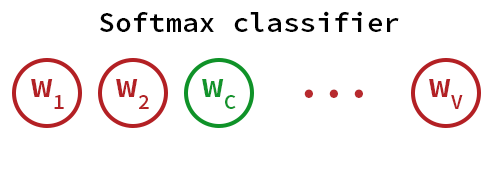
\includegraphics[width=0.9\linewidth]{Images/discri-softmax.png}
        \caption{Softmax loss}
    \end{subfigure}
    \begin{subfigure}{.5\textwidth}
        \centering
        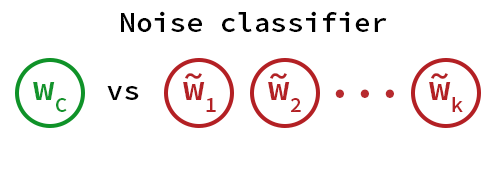
\includegraphics[width=0.9\linewidth]{Images/discri-noise.png}
        \caption{Negative Sampling loss}
    \end{subfigure}
    \caption{Comparison of the two loss functions}
    \label{discri}
\end{figure}

The new binary classification task has $w_c$ as positive example $(y=1)$ and all the noise samples $\tilde{w}_1, \tilde{w}_2, ..., \tilde{w}_k$  as negative examples $y=0$. The loss function, with a pair $(w_t, w_c)$, is:
\begin{equation}
    \text{J}_{\text{NEG}}  = -[\text{log}~P(y=1| w_c, w_t) + k\mathbb{E}_{\tilde{w}\sim Q}[\text{log}~P(y=0|\tilde{w}, w_t]]
\end{equation}

Calculating the expectation $\mathbb{E}_{\tilde{w}\sim Q}$ would involve summing over all the vocabulary to compute the probability normalising constant, which is exactly what we wanted to avoid in the first place. That's why we will instead use a Monte Carlo approximation with our noise samples:
\begin{align}
    \text{J}_{\text{NEG}}  &= -\left[\text{log}~P(y=1| w_c, w_t) + k\sum_{j=1}^{k}\frac{1}{k}\text{log}~P(y=0|\tilde{w}_j, w_t]\right]\nonumber \\
     &= -\left[\text{log}~P(y=1| w_c, w_t) + \sum_{j=1}^k\text{log}~P(y=0|\tilde{w}_j, w_t)\right]
\end{align}

We still haven't a proper derivation of the probability $P(y=1| w_c, w_t)$. Note that for each context word $w_c$ given its target word $w_t$, we're generating $k$ noise samples from a distribution $Q$. There are two distributions at stake: the distribution $P_{\text{train}}$ of the context word $w_c$ given $w_t$ which is simply the softmax computed earlier:
\begin{equation}
    P_{\text{train}}(w_c|w_t) = \text{softmax}(w_c, w_t)
\end{equation}
And the unigram distribution $Q$ to sample the noise:
\begin{equation}
    Q(w_i) = \frac{f_i^{3/4}}{\sum_{j=1}^V f_j^{3/4}}
\end{equation}

The probability to obtain a positive example is simply a weighted probability of seeing an example from $P_{\text{train}}$:
\begin{align}
    P(y=1| w_c, w_t) &= \frac{\frac{1}{k+1}P_{\text{train}}(w_c|w_t)}{\frac{1}{k+1}P_{\text{train}}(w_c|w_t) + \frac{k}{k+1}Q(w_c)}\nonumber \\
     &= \frac{P_{\text{train}}(w_c|w_t)}{P_{\text{train}}(w_c|w_t) + kQ(w_c)}
\end{align}

Therefore we also have:
\begin{equation}
    P(y=0| w_c, w_t) = \frac{kQ(w_c)}{P_{\text{train}}(w_c|w_t) + kQ(w_c)}
\end{equation}

Computing $P_{\text{train}}(w_c|w_t)$ remains expensive as it involves the softmax normalising factor $Z(w_c)$:
\begin{align}
    P_{\text{train}}(w_c|w_t) &= \frac{\text{exp}\{\text{score}(w_c, w_t)\}}{\sum_{\text{Word w' in Vocab}}\text{exp}\{\text{score}(w_c, w')\}} \nonumber \\
     &= \frac{\text{exp}\{\text{score}(w_c, w_t)\}}{Z(w_c)}
\end{align}

The trick to avoid computing $Z(w_c)$ is to simply consider it as another parameter the model has to learn. Mnih and Teh \cite{nce} actually set the parameter to 1 as they report that it doesn't affect the performance. This statement was bolstered by Zoph et al. \cite{nce2} who found that the parameter was close to 1 with a low variance. Setting $Z(w_c)$ to 1 gives:
\begin{equation}
    P(y=1| w_c, w_t) = \frac{\text{exp}\{\text{score}(w_c, w_t)\}}{\text{exp}\{\text{score}(w_c, w_t)\} + kQ(w_c)}
\end{equation}

The loss function becomes:
\begin{equation}
    \text{J}_{\text{NEG}}  = -\left[\text{log}~\frac{\text{exp}\{\text{score}(w_c, w_t)\}}{\text{exp}\{\text{score}(w_c, w_t)\} + kQ(w_c)} + \sum_{j=1}^k\text{log}~\frac{kQ(\tilde{w}_j)}{\text{exp}\{\text{score}(\tilde{w}_j, w_t)\} + kQ(\tilde{w}_j)}\right]
\end{equation}

Actually, this loss function is not quite Negative Sampling, but instead what we call Noise Contrastive Estimation (NCE), Negative Sampling has a further simplification we'll discuss shortly. Mnih and Teh \cite{nce} proved that as the number of noise samples $k$ increases, the gradient of the derivative of the NCE goes toward the softmax function. In their paper, they also state that 25 samples are enough to match the performance of the softmax, but with an increased speed of 45.

The remaining expensive term to compute in the loss function is $kQ(w_c)$, as it involves computing the unigram distribution over all the vocabulary. This isn't as expensive as the normalising factor $Z(w_c)$ as the noise distribution only need to be computed once and stored in a matrix during the whole training. However, in Negative Sampling, this most expensive term $kQ(w_c)$ is set to 1 \cite{word2vec2}. This is actually true when $k=V$ and $Q$ is an uniform distribution.	 Now $P(y=1| w_c, w_t)$ is actually a sigmoid function:
\begin{equation}
    P(y=1| w_c, w_t) = \frac{1}{1 + \text{exp}\{-\text{score}(w_c, w_t)\}}
\end{equation}

Giving the following final loss function:
\begin{equation}
    \text{J}_{\text{NEG}} = -\left[\text{log}~\frac{1}{1 + \text{exp}\{-\text{score}(w_c, w_t)\}} + \sum_{j=1}^k\text{log}~\frac{1}{1 + \text{exp}\{\text{score}(\tilde{w}_j, w_t)\}}\right]
\end{equation}

\subsection{Word Pairs and Phrases}
`Times Higher Education' has a different meaning than `times', `higher' and `education' taken separately, it's therefore sensible to add that kind of phrases in the vocabulary. Ideally, we would like to also not add word pairs such as `that is' or `and are' to the vocabulary as they make more sense being separated. We want to group words that are frequent together but infrequent in general, to do so, we use the following scoring function of two words $w_i$ and $w_j$:
\begin{equation}
    \text{score}(w_i, w_j) = \frac{\text{count}(w_iw_j) - \delta}{\text{count}(w_i)\times \text{count}(w_j)}\times |W|
\end{equation}
With: 
\begin{itemize}[topsep=0pt]
    \item $\text{count}(w_i)$ the number of time the word $w_i$ appear in the corpus (all the training data).
    \item $\text{count}(w_iw_j)$ the number of occurrence of both $w_i$ and $w_j$ in the corpus. 
    \item $\delta$ a discounting coefficient to prevent too many phrases made up of very infrequent words.
    \item $|W|$ the training set size, in order to make the threshold more independent of the training size.
\end{itemize}

The pairs $(w_i, w_j)$ with a score above a threshold are then added to the vocabulary. Several passes on the training data are made to make longer phrases such as `Times Higher Education' (usually 2-4 passes with a decreasing threshold value after each pass).

\subsection{Subsampling of Frequent Words}
If we look again at the example `the ants in the garden', the training instances will contain (ants, the) and (garden, the). The word `the' doesn't help a lot at understanding the usual context of the words `ant' and `garden' as it appears in virtually every noun. Furthermore, `the' will have far too many training instances to get a vector representation of that word.

To address these problems, subsampling was used: each word in the corpus has a probability to be deleted relative to its frequency. Therefore, if we have a window size of 15 and the word `the' is deleted, then this word will not appear in the context of the remaining words. Also, we now have 15 times fewer training instances containing `the'.

The probability of keeping a word $w_i$ with frequency $f_i$ is:
\begin{equation}
    P(w_i) = \frac{t}{f_i} + \sqrt{\frac{t}{f_i}}
    \label{subsampling}
\end{equation}
With $t$ a parameter controlling how aggressive subsampling is, smaller value of $t$ means more subsampling. 

\begin{figure}[H]
    \centering
    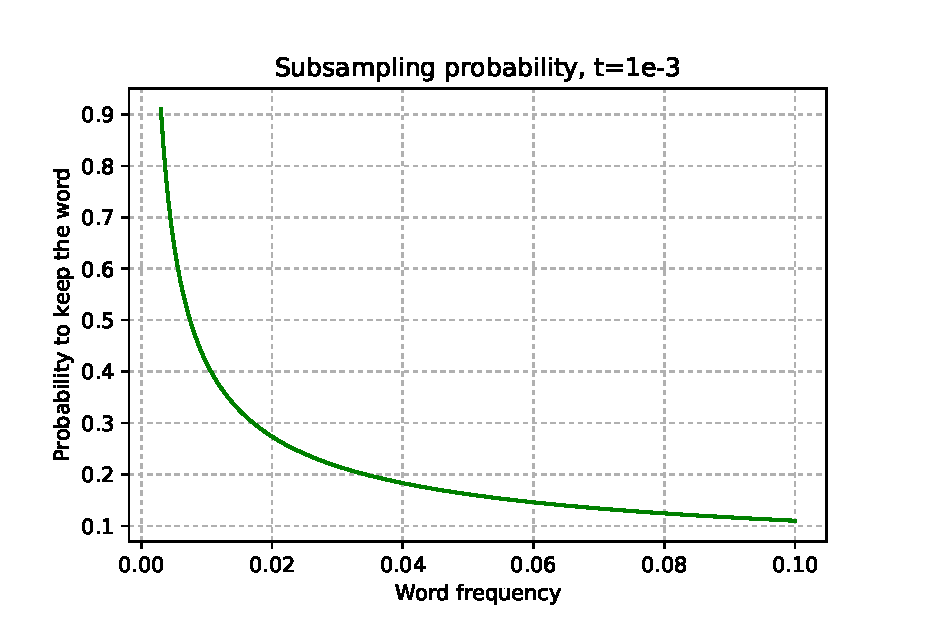
\includegraphics[width=0.8\textwidth]{Images/subsampling_prob.eps}
    \caption{Subsampling probability graph}
\end{figure}

Note that the formula (\ref{subsampling}) is different from the one in \cite{word2vec2}, but we decided to keep (\ref{subsampling}) as it was used in the actual C implementation of Word2Vec. Note that if $t=1\mathrm{e}{-3}$
\begin{itemize}
    \item $P(w_i) = 1.0$ for $f_i\leq0.0026$, meaning that subsampling will only affect words that represent more than 0.26\% of the words.
    \item $P(w_i) = 0.5$ for $f_i=0.0075$, any word representing 0.75\% of the words will have a fifty-fifty chance of being dropped.
\end{itemize}

\subsection{Word2Vec Pre-Trained Model}

For our task of emotion prediction, we will be using a pre-trained model to convert the text in Tumblr posts into rich high-dimensional vectors. The model was trained on Google News dataset (aggregation of news from all around the world) containing about 100 billion words. Each word in the vocabulary (3 million words) are embedded into a 300 dimensional vector. 

The skip-gram model had the following parameters:
\begin{itemize}
    \item Context window size of 10.
    \item 5 negative examples for Negative Sampling.
    \item In Word Pairs and Phrases, $\delta$ is equal to 100, and the threshold is set to 100. The number of passes was not found [need to look].
    \item Subsampling threshold of $1\mathrm{e}{-3}.$
\end{itemize}

\section{Results}
Each post in the dataset does not necessarily contain the same number of words. Even after embedding each word, the input will be of variable size and most learning algorithm expect a fixed-sized input. To solve that problem, we can simply average across the number of words. The information loss is still minimal as the features come from a high-dimensional space \cite{seth1} [Elaborate on mean embedding].

The network architecture is straight-forward as the output softmax layer directly follows the mean embedding [illustration required]. This model achieves \textbf{55\%} accuracy on the test set. This is not bad at all, but note that the word order is completely lost! The order can be preserved using Recurrent Neural Networks, which is our next section.






\chapter{Recurrent Neural Networks}

Recurrent Neural Networks (RNN) can be used in a wide variety of tasks as they can work with inputs and outputs of variable size.
\begin{figure}[H]
    \centering
    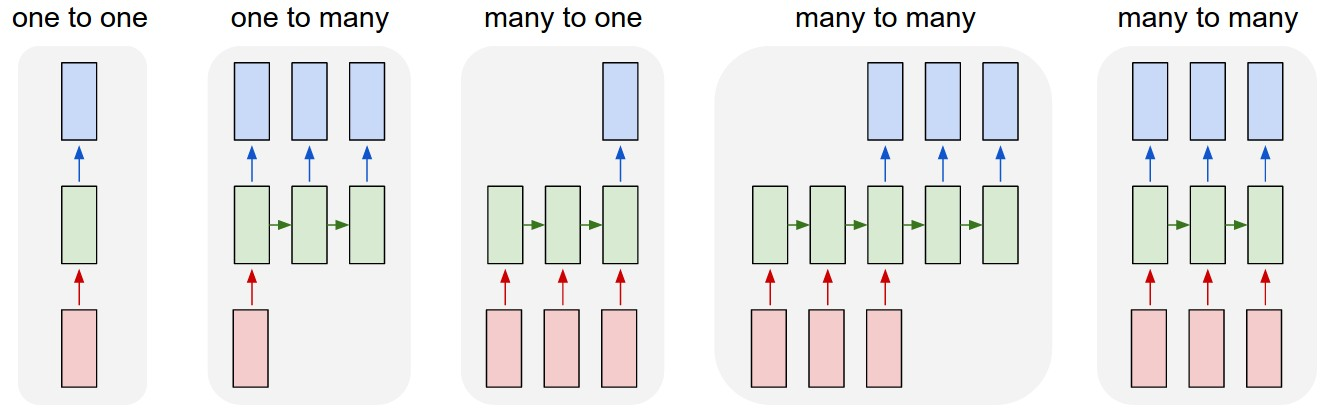
\includegraphics[width=\textwidth]{Images/rnn.jpeg}
    \caption{The applications of Recurrent Neural Networks \cite{unres-rnn}}
\end{figure}

\begin{enumerate}
     \itemsep0em
     \item \textbf{One to one}: A vanilla neural network with fixed-sized input and fixed-sized output.
     \item \textbf{One to many}: An RNN with sequence output, e.g. image captioning: generate a sentence describing an input image.
     \item \textbf{Many to one}: An RNN with sequence input, e.g. sentiment analysis: infer the emotion of a given sentence.
     \item \textbf{Many to many (1)}: Sequence input and sequence output, e.g.: machine translation: output a sentence in Spanish given a sentence in English.
     \item \textbf{Many to many (2)}: Synced sequence input and output, e.g.: video classification: label each frame of a video.
\end{enumerate}

%%%%%%%%%%%%%%%%%%%%%%%%%%%%%%%%%%%%%%%%%%%%%%%%%%%%%%%%%%%%
%%%%%%%%%%%%%%%%%%%%  NEW SECTION   %%%%%%%%%%%%%%%%%%%%%%%%
%%%%%%%%%%%%%%%%%%%%%%%%%%%%%%%%%%%%%%%%%%%%%%%%%%%%%%%%%%%%
\section{Vanilla RNN}
Traditional neural networks do not have any memory as each input of the network are independent. Recurrent neural networks use loops to make information persist as shown on Figure (\ref{vanilla-rnn}).

\begin{figure}[H]
    \centering
    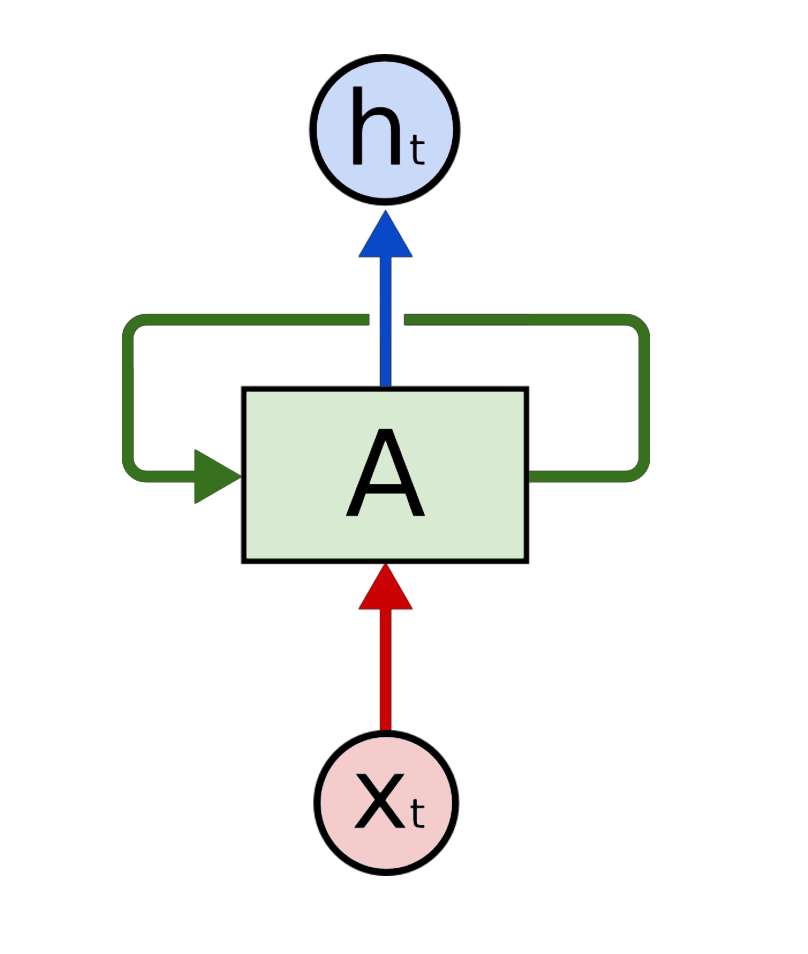
\includegraphics[width=0.3\textwidth]{Images/vanilla-rnn.png}
    \caption{A vanilla recurrent neural network \cite{colah}}
    \label{vanilla-rnn}
\end{figure}

Given an input $x_t$ and a layer $A$, the output $h_t$ is fed again to the layer along with the next input $x_{t+1}$. This becomes clearer when we unroll the RNN:

\begin{figure}[H]
    \centering
    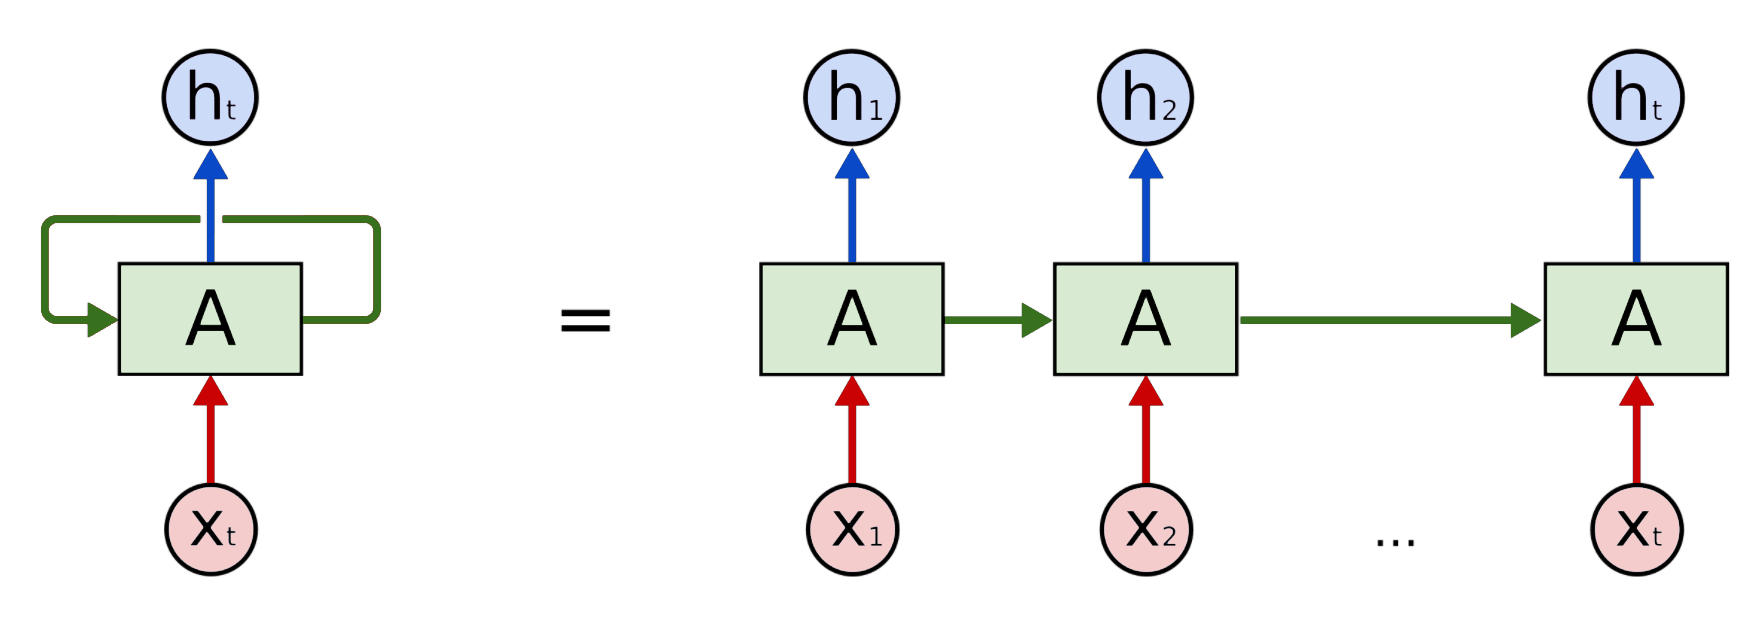
\includegraphics[width=\textwidth]{Images/vanilla-rnn2.png}
    \caption{An unrolled vanilla recurrent neural network \cite{colah}}
\end{figure}

Basically, if we denote the function of the layer A by $f$:
\begin{equation}
    h_t = f(h_{t-1}, x_t)
\end{equation}

Suppose the input $x_t \in \mathbb{R}^{D}$ and the layer $A$ contains $H$ neurons. Denote $W_x \in \mathbb{R}^{D\times H}$ the weights of the input, and $W_h \in \mathbb{R}^{H\times H}$ the weights of the hidden state. Usually $f$ is simply:
\begin{equation}
    h_t = \text{tanh}(W_x x_t + W_h h_{t-1})
\end{equation}

Just like the layer traditional neural network with a tanh (hyperbolic tangent) activation function and two inputs instead of one.

\begin{figure}[H]
    \centering
    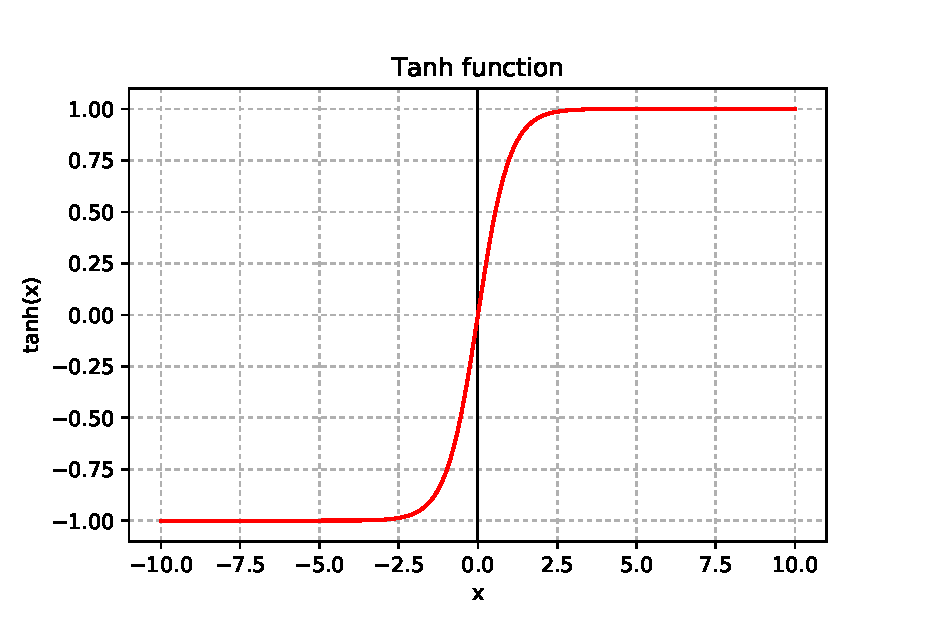
\includegraphics[width=0.5\textwidth]{Images/tanh.eps}
    \caption{Another activation function: tanh}
\end{figure}

This vanilla RNN is a good step towards learning from sequential inputs but most people use a variant called Long-Short Term Memory (LSTM) that work extremely well on many different tasks. 

\section{Long-Short Term Memory Networks}
The vanilla RNN is hard to train as the gradients often either vanish or explode. That's because during backpropagation, the weights $W_x$ and $W_h$ go through repeated matrix multiplication [detail the maths] than can either make them go to zero or diverge. LSTMs solve this problem by using a gating mechanism. 

They keep track of the hidden state vector $h_t \in \mathbb{R}^H$ but also of a cell state vector $c_t\in \mathbb{R}^H$, we'll shortly explain. First, we compute the activation vector $a \in \mathbb{R}^{4H}$ that is 4 times bigger than vanilla RNN, which is necessary to remember long and short-term features. 
\begin{equation}
a = W_x x + W_h h
\end{equation}
with $x \in \mathbb{R}^{D}$, the input, $h \in \mathbb{R}^{H}$, the hidden state, $W_x \in \mathbb{R}^{D\times 4H}$ and $W_h \in \mathbb{R}^{H\times 4H}$.

Then this activation vector $a$ is split into 4: $a_i, a_f, a_o, a_g \in \mathbb{R}^H$, where $a_i$ is made up of the first $H$ elements of $a$, $a_f$ the $H$ next, etc. Now we compute the input gate $i \in \mathbb{R}^H$, the forget gate $f \in \mathbb{R}^H$, the output gate $o \in \mathbb{R}^H$ and the block input $g \in \mathbb{R}^H$ as: 
\begin{equation}
    i = \sigma(a_i) \qquad f = \sigma(a_f) \qquad o = \sigma(a_o) \qquad g = \text{tanh}(a_g)
\end{equation}
where $\sigma$ is the sigmoid function.

Finally, we can compute the new cell state and the new hidden state as follow:
\begin{equation}
     c_t = i\odot g + f\odot c_{t-1} \qquad h_t = o\odot \text{tanh}(c_t)
\end{equation}
where $\odot$ is the elementwise product of vectors.
$c_t$ is the sum of:
\begin{itemize}
    \item The new information $g$ weighted by how much we want to add that new information with $i$ (remember that the sigmoid function has values between 0 and 
    1).
    \item What we knew before, $c_{t-1}$, weighted by how much we want to forget long-term information with $f$.
\end{itemize} 
That cell state then goes through a tanh activation function (just like in the vanilla RNN) and is multiplied by the output gate $o$ that decide how much to let through the next state. 

LSTMs therefore manage to easily remember long-term dependencies, as well as short-term ones, thus its name.

Also, note that the activation function in recurrent neural networks is a tanh and not a ReLU. ReLU was originally introduced to replace tanh because of the vanishing gradient problem. However, in the case of recurrent networks, LSTMs are built to not have vanishing gradients, which makes ReLU unnecessary.

\newpage
\section{LSTM for Sentiment Analysis}
We'll be using the following architecture:

\begin{figure}[H]
    \centering
    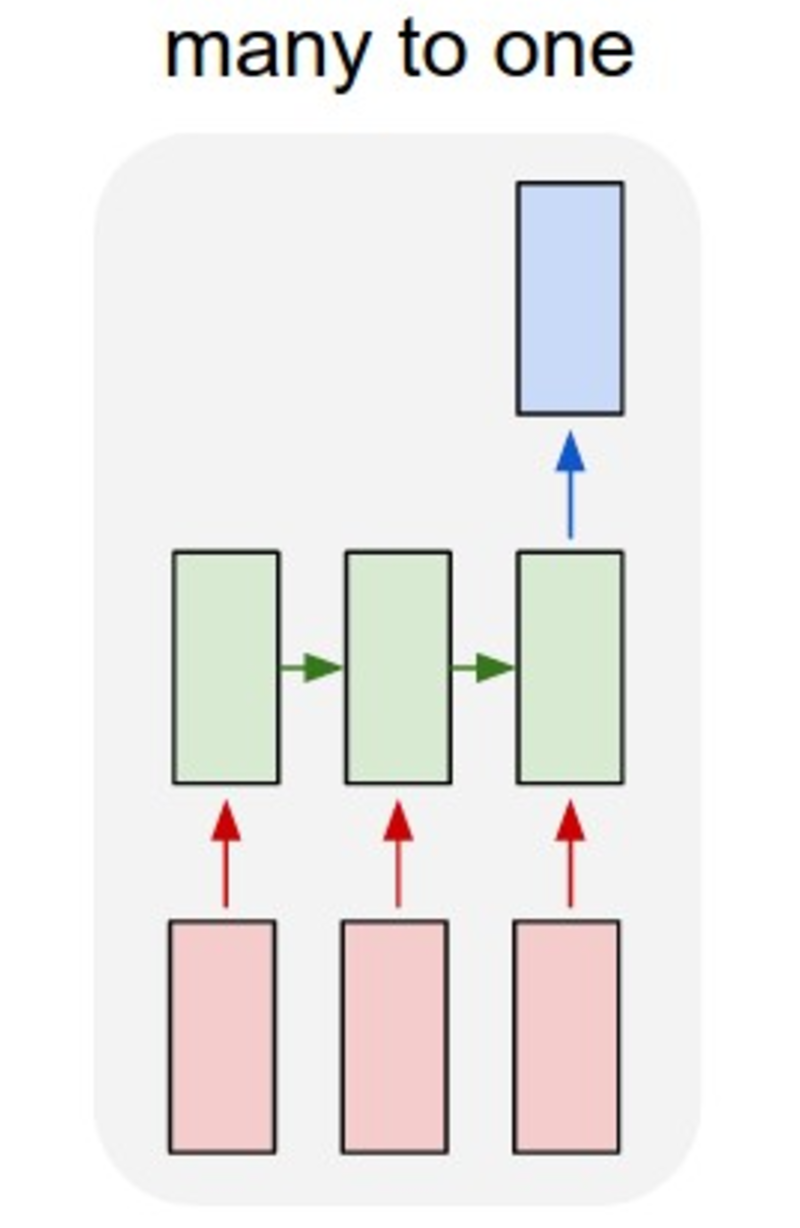
\includegraphics[width=0.3\textwidth]{Images/many-to-one.png}
    \caption{Many to one architecture}
\end{figure}

Each post will be broken down into a sequence of words and then fed to the LSTM that will infer the emotion of the user. On a more technical note, the vector of words will be represented by a list of ids from the Word2Vec vocabulary say $[3, 20, 1, 49, 6]$. To account for shorter posts, we'll have to zero-pad the vector -- the id 0 will actually be associated with a word token $<$PAD$>$ -- as $[3, 20, 1, 49, 6, 0, 0, ..., 0]$. The LSTM will then give the prediction by stopping before the zero-padding.

\section{Results}
(upcoming)








\chapter{Deep Sentiment}

Real-world information oftentimes come in several modalities. For instance, in speech recognition, humans integrate audio and visual information to understand speech, as was demonstrated by the McGurk effect \cite{mcgurk}. Separating what we see from what we hear seems like an easy task, but in an experiment conducted by McGurk, the subjects who were listening to a /{\em ba}/ sound with a visual /{\em ga}/ actually reported they were hearing a /{\em da}/. This is uncanny as even if we know the actual sound is a /{\em ba}/, we cannot stop our brain from interpreting it as a /{\em da}/.

Likewise, an image almost always come with a text as different interpretation can arise when a textual context is not provided, as shown in Figure \ref{ambiguous}:

\begin{figure}[H]
    \begin{subfigure}{.5\textwidth}
        \centering
        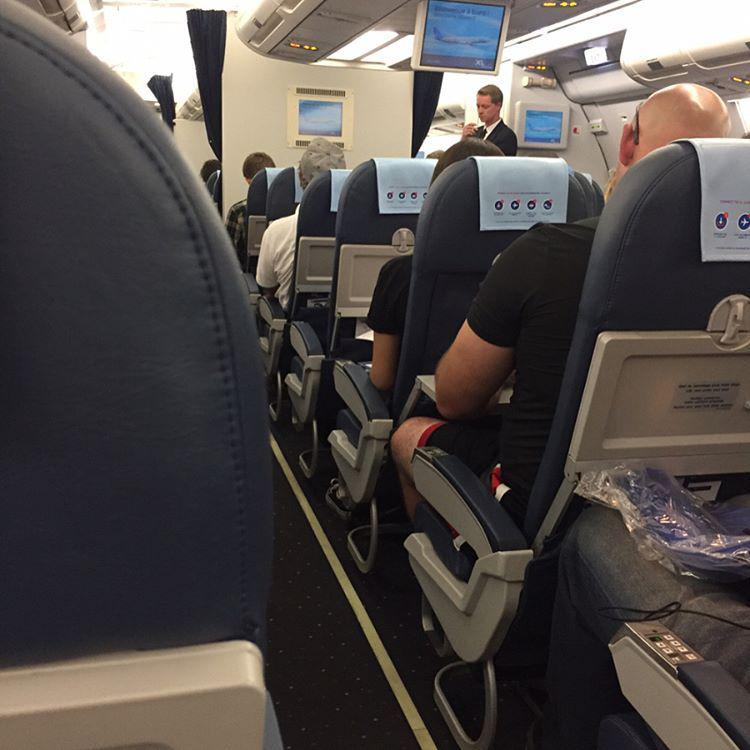
\includegraphics[width=0.9\linewidth]{Images/scared.jpg}
        \caption{``Planes might just be the most frightening thing ever." \textbf{scared}}
    \end{subfigure}
    \begin{subfigure}{.5\textwidth}
        \centering
        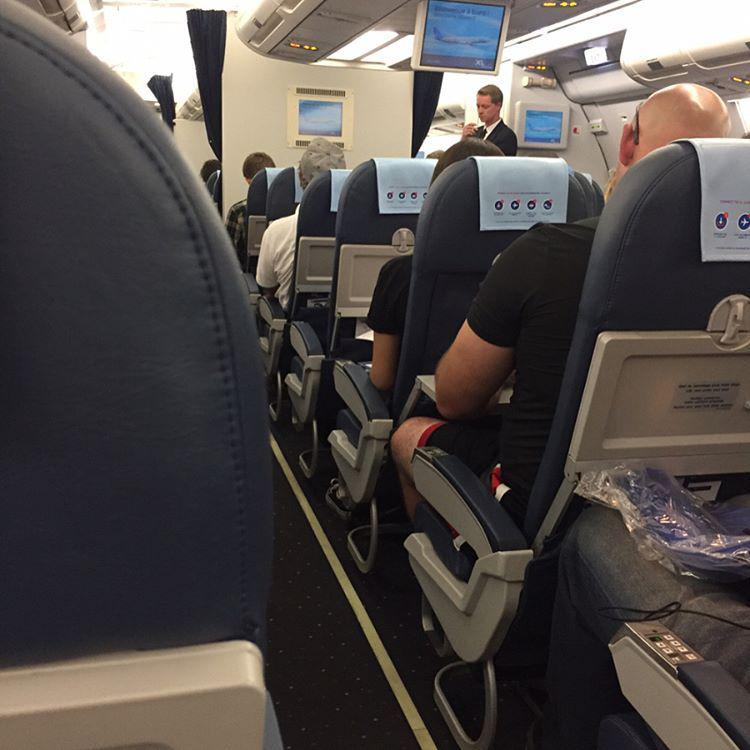
\includegraphics[width=0.9\linewidth]{Images/scared.jpg}
        \caption{``I hate it when people are taking too much space on planes." \textbf{angry}}
    \end{subfigure}
    \caption{Different meanings with different captions.}
    \label{ambiguous}
\end{figure}

Exploiting both visual and textual information is therefore key to understand the user's emotional state. Deep Sentiment is the name of the deep neural network incorporating visual recognition and text analysis.

%%%%%%%%%%%%%%%%%%%%%%%%%%%%%%%%%%%%%%%%%%%%%%%%%%%%%%%%%%%%
%%%%%%%%%%%%%%%%%%%%  NEW SECTION   %%%%%%%%%%%%%%%%%%%%%%%%
%%%%%%%%%%%%%%%%%%%%%%%%%%%%%%%%%%%%%%%%%%%%%%%%%%%%%%%%%%%%
\section{Model Architecture}

Deep Sentiment builds on the models we have seen before as shown in Figure \ref{deep-sentiment}:

\begin{figure}[H]
    \centering
    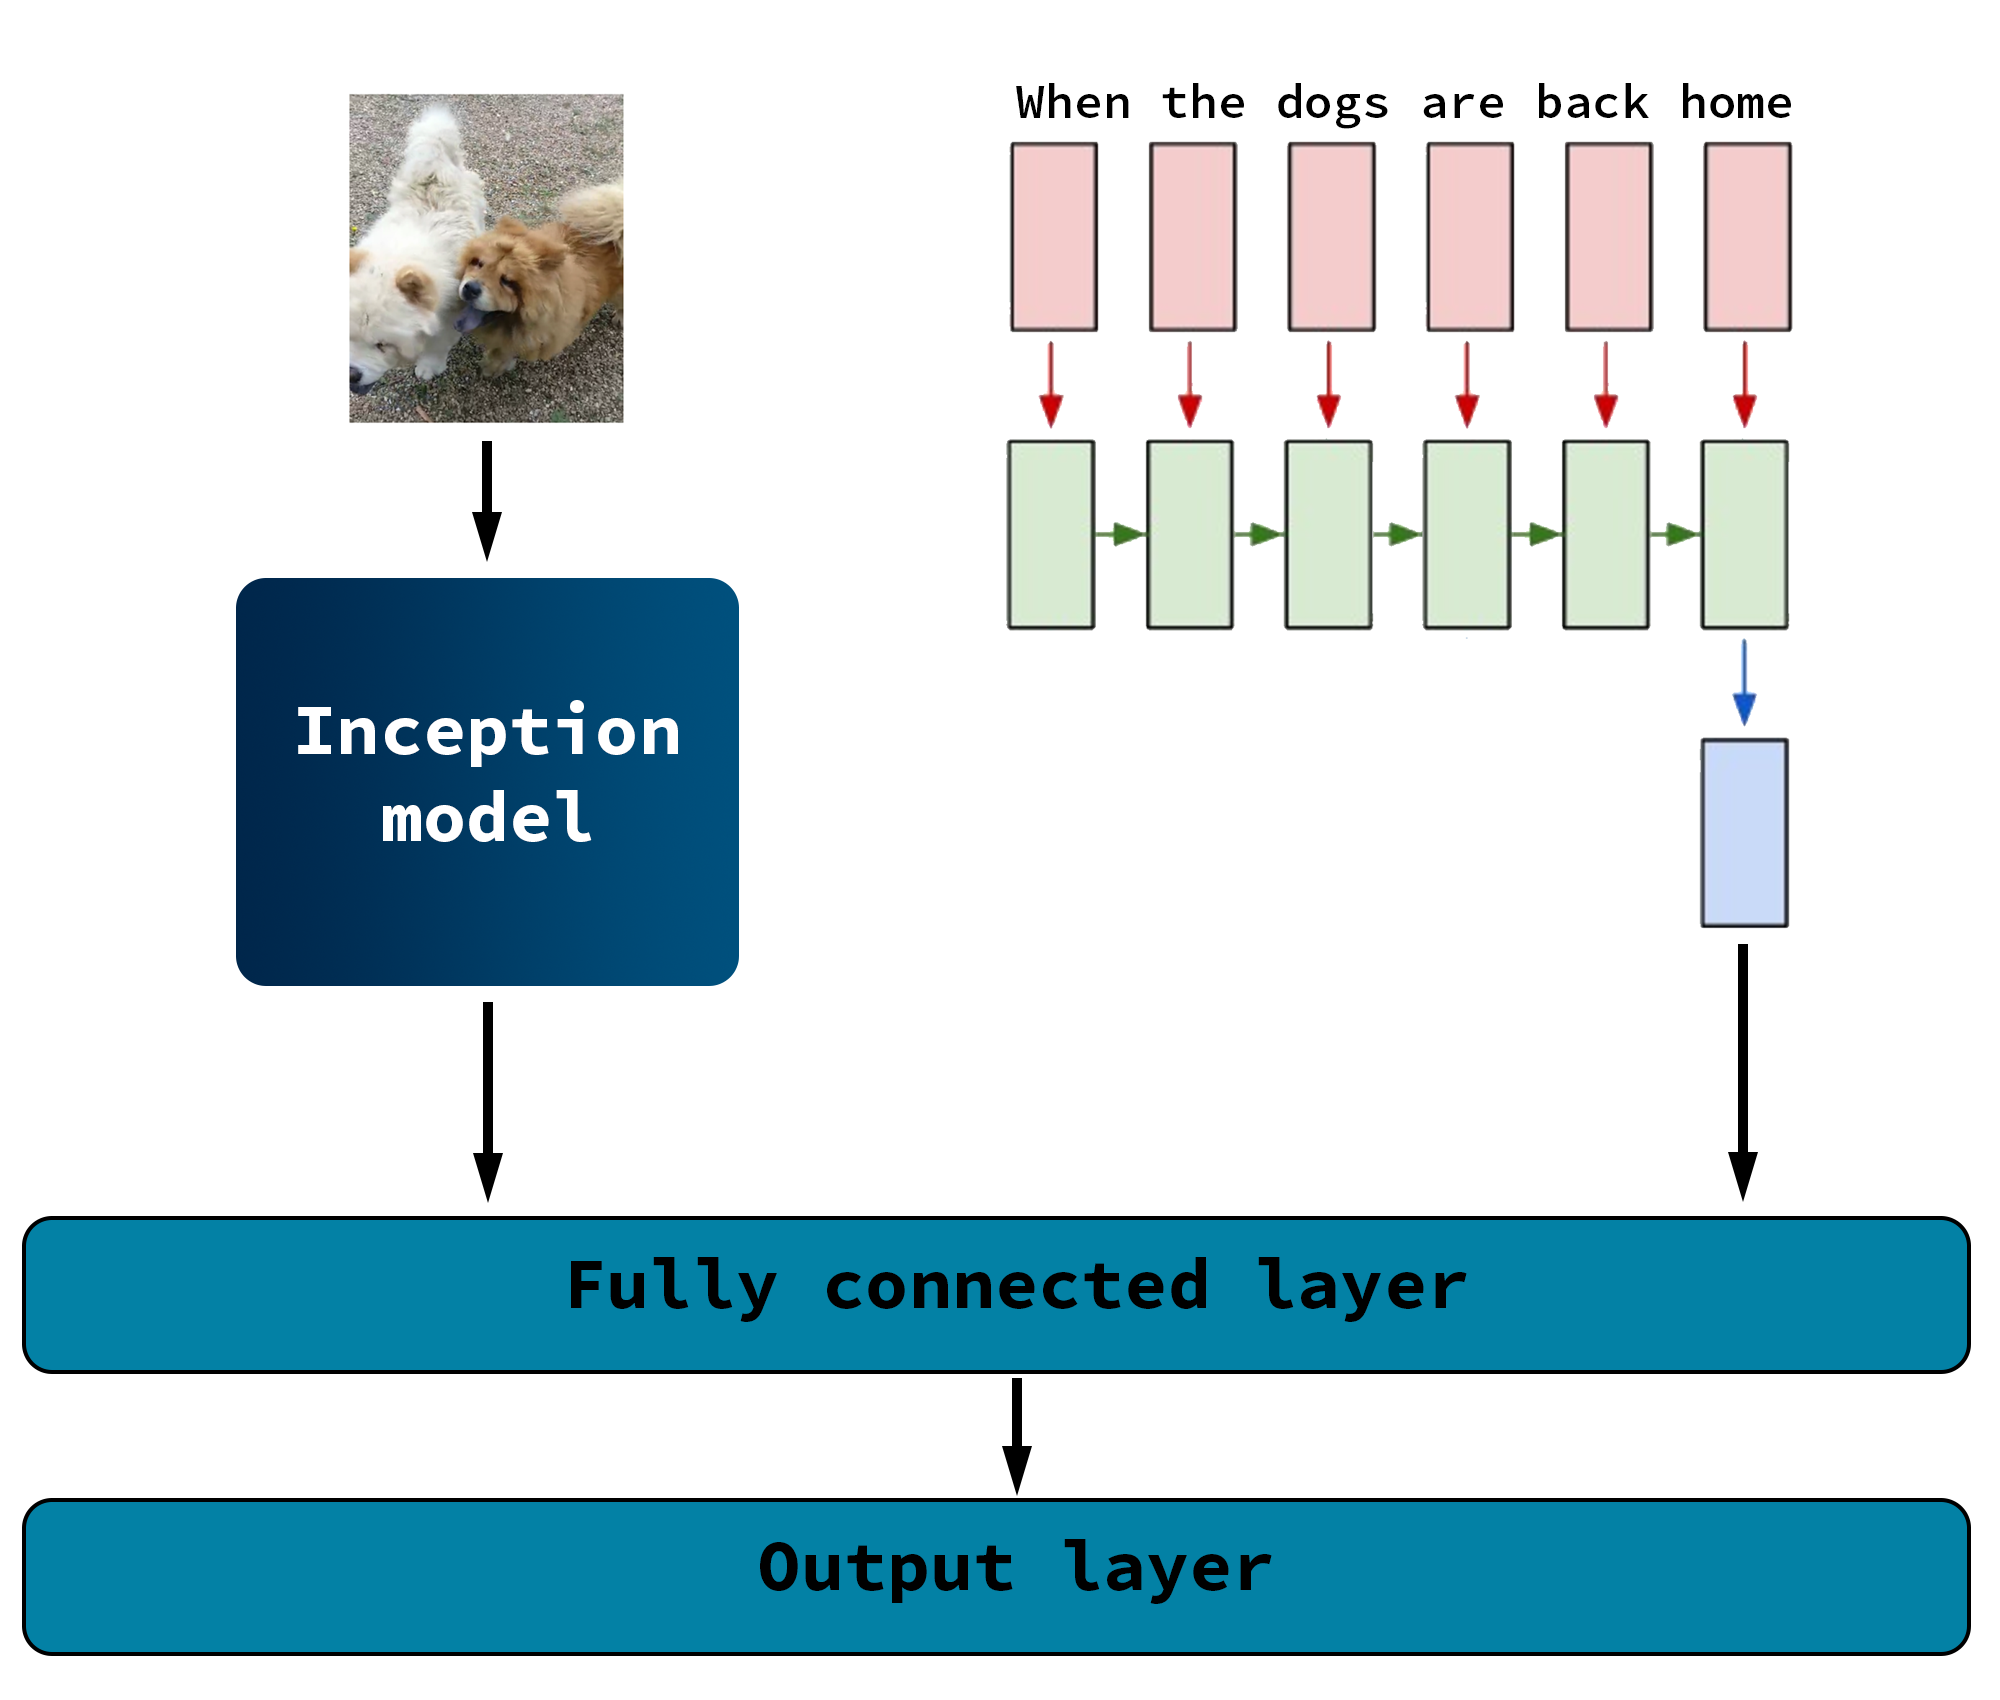
\includegraphics[width=\textwidth]{Images/deep-sentiment.png}
    \caption{Deep Sentiment architecture}
    \label{deep-sentiment}
\end{figure}

\begin{enumerate}
    \item The image go through the pre-trained Inception model that will extract features from the images: more precisely with 128 neurons in the last Inception 
    layer.
    \item The text is embedded in a high-dimensional space with Word2Vec and will be fed to an LSTM with a 2048 neurons output layer.
    \item The two outputs are concatenated (size 128 + 2048 = 2176 ) and fed to a fully connected layer with 1024 neurons. 
    \item The final layer contains 6 neurons, one for each basic emotion.
    \item Softmax is applied to the final layer to give the probability distribution of the emotional state of the user.
\end{enumerate}

\section{Results}
Deep Sentiment was trained with:
\begin{itemize}[topsep=0pt]
    \itemsep-1em
    \item 10,000 training steps
    \item Mini-batch size of 32
    \item Adam optimizer with an initial learning rate of $1\mathrm{e}{-3}$
    \item Learning rate decay of $\frac{1}{2}$ every 1000 steps
\end{itemize}

The training process of the Inception fine-tuning was monitored with Tensorboard:
\begin{figure}[H]
    \centering
    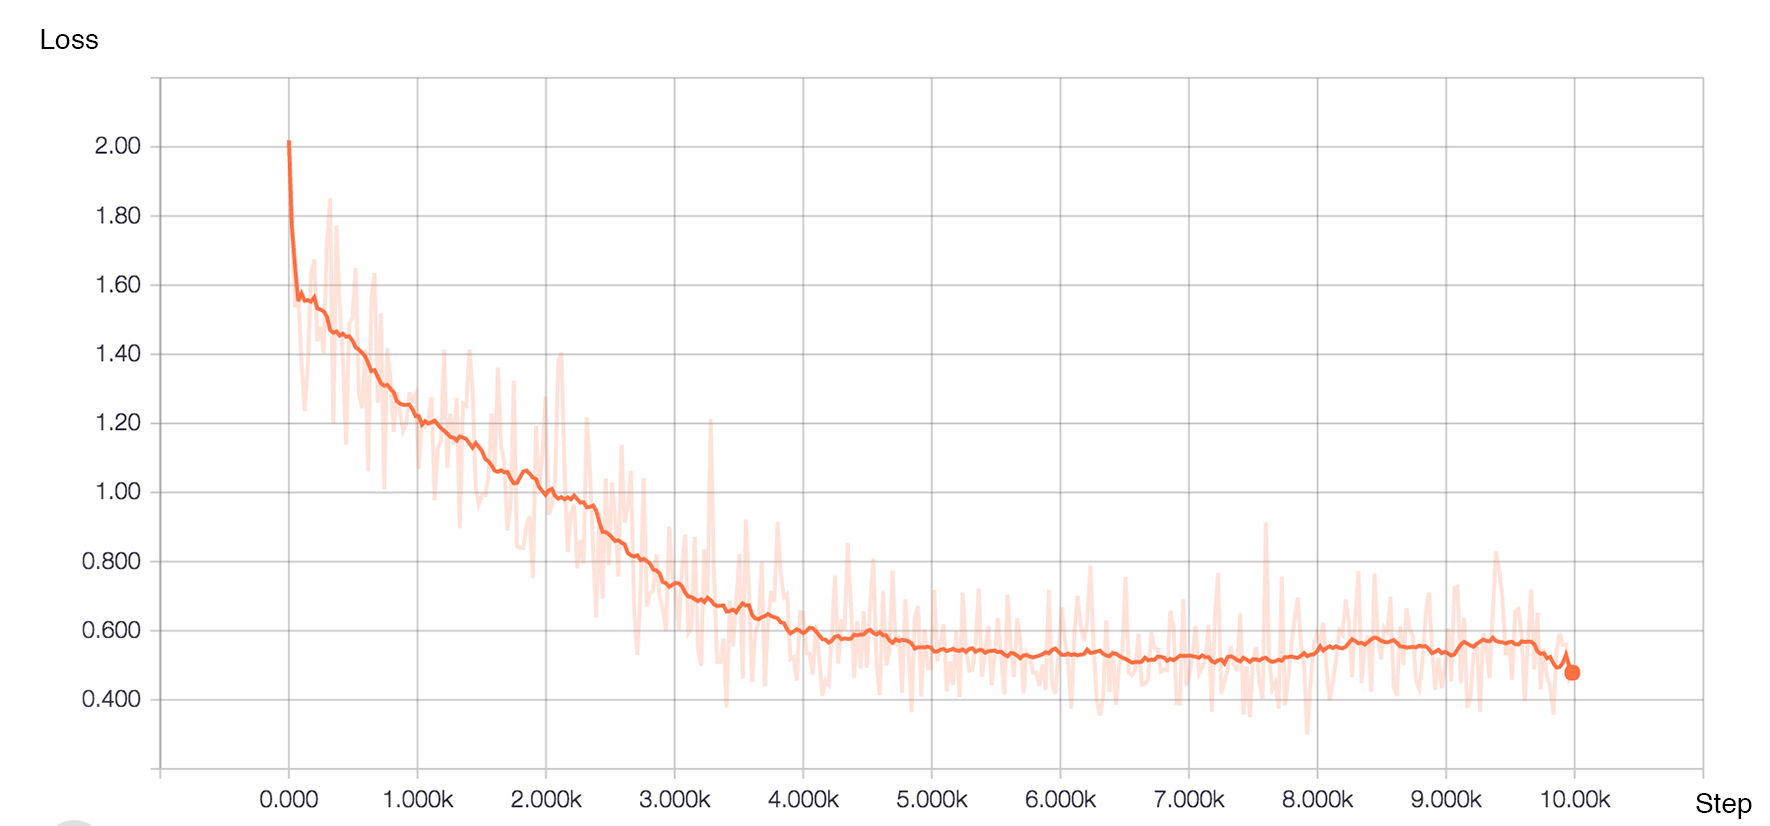
\includegraphics[width=\textwidth]{Images/image_text_model_loss_cleaned.jpg}
    \caption{Loss function of Deep Sentiment}
\end{figure}

\begin{figure}[H]
    \centering
    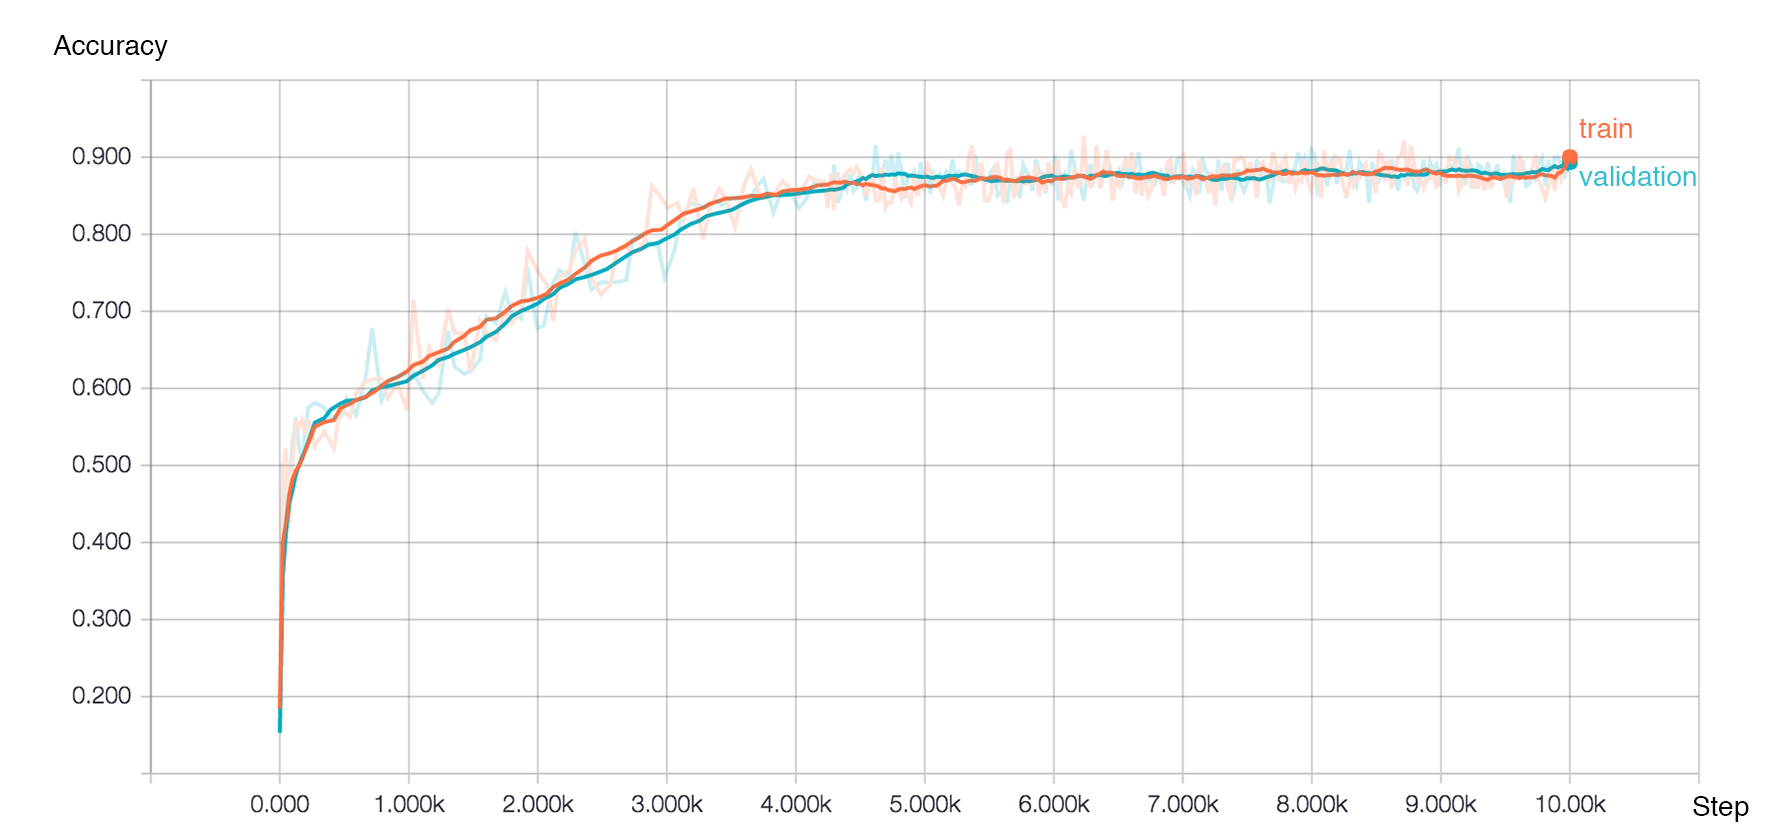
\includegraphics[width=\textwidth]{Images/image_text_model_accuracies_cleaned.jpg}
    \caption{Train/validation accuracies of Deep Sentiment}
\end{figure}

This model combining text and image vastly outperforms the algorithms only using those elements separately with 90\% train accuracy and 89\% test accuracy. This shows that just like a human being, a neural network needs both visual and textual information to determine the emotion conveyed by a post. The synergy between visual recognition and natural language processing is impressive as shown in the comparison table \ref{all-results}.

\begin{table}[H]
\begin{center}
    \begin{tabular}{| l | c | c | c |}
    \hline
    & \textbf{Loss} & \textbf{Train} & \textbf{Test} \\
    & & \textbf{accuracy} & \textbf{accuracy} \\ \hline
    \textbf{Random guessing} & - & 24\% & 24\% \\ \hline
    \textbf{Inception fine-tuned}  & 1.61 & 48\% & 42\% \\ \hline
    \textbf{LSTM word embedding} & 1.01 & 61\% & 63\% \\ \hline
    \textbf{Deep Sentiment} & \textbf{0.48} & \textbf{90\%} & \textbf{89\%} \\
    \hline
    \end{tabular}
\end{center} 
\caption{Comparison of results}
\label{all-results}
\end{table}

\newpage
\section{Emotion visualisation}
We can generate an image that maximises the score of a certain emotion by performing gradient ascent on a randomly initialised image \cite{class-vis}.

More concretely, let $I$ be an image and $y$ be a target emotion. Let us denote by $s_y(I)$ the score of class $y$ for the image $I$, that is one of the six neurons right before the softmax layer. We want to generate an image with a high score for emotion $y$ by solving the problem:
\begin{equation}
I^* = \text{arg\,max}_I ~s_y(I) - R(I)
\end{equation}

with $R(I)$ a regulariser that contains both explicit and implicit regularisation we will describe shortly.

Note that we're maximising the unnormalised class scores $s_y(I)$ and not the probabilities returned by the softmax: $\frac{s_y(I)}{\sum_c s_c(I)}$. The reason is that maximising the softmax probabilities can be achieved by minimising the scores of the other emotions. Instead, we want to make sure the optimisation concentrates on the emotion we want to visualise. 

\subsection{Regularisation}

The explicit regulariser is the $L_2$ decay: $R(I) = \lambda \Vert I \Vert_2^2$ that prevents extreme pixel values from dominating the generated image. Those pixel values do not occur naturally in real images and are not useful for visualisation.

The implicit regularisations are: \cite{class-vis2}
\begin{enumerate}
    \item \textbf{Gaussian blur:} Gradient ascent tends to produce image with high frequency information. What are frequencies in images? To put it simply, each image 
    is made of various frequencies: start with the average colour (low frequency) and slowly add higher frequencies wavelengths to build the details of the image.
    
    An image with high frequency information causes high activations but are not realistic nor interpretable as shown by Nguyen et al. \cite{nguyen}. High frequency 
    information are penalised using a Gaussian blur step on image $I: \text{GaussianBlur}(I, \theta_{\text{blur}})$ with $\theta_{\text{blur}}$ the standard deviation of the 
    Gaussian kernel used in the blur step. Blurring an image is computationally expensive and as such, we're only blurring every $\theta_{\text{blur-every}}$ steps.
    \item \textbf{Pixel clipping:} After performing $L_2$ decay and Gaussian blur, that suppress high amplitude and high frequency information, we're left with images 
    with pixel values that are small and smooth. However, each pixel will still be non-zero and contribute a little bit to the gradient. We want to discard the contribution of 
    unimportant pixels and focus only on the main object. That can be done by setting pixels with small norm (over the red, green, blue channels) to zero. The threshold  
    $\theta_{\text{small-norm}}$ for the norm is set to be a percentile of all pixel norms in the image.
\end{enumerate}

\subsection{Generated images}

We performed gradient ascent on a randomly initialised image using the following parameters:
\begin{itemize}
    \item $L_2$ regularisation parameter: $\lambda = 0.001$.
    \item In Gaussian blur, $\theta_{\text{blur}} = 0.5$ and $\theta_{\text{blur-every}} = 10$.
    \item In pixel clipping, $\theta_{\text{small-norm}}$ is the norm of the $10^{\text{th}}$ percentile.
    \item 500 gradient updates.
\end{itemize}

Maximising over the emotion `happy' yielded:

\begin{figure}[H]
    \centering
    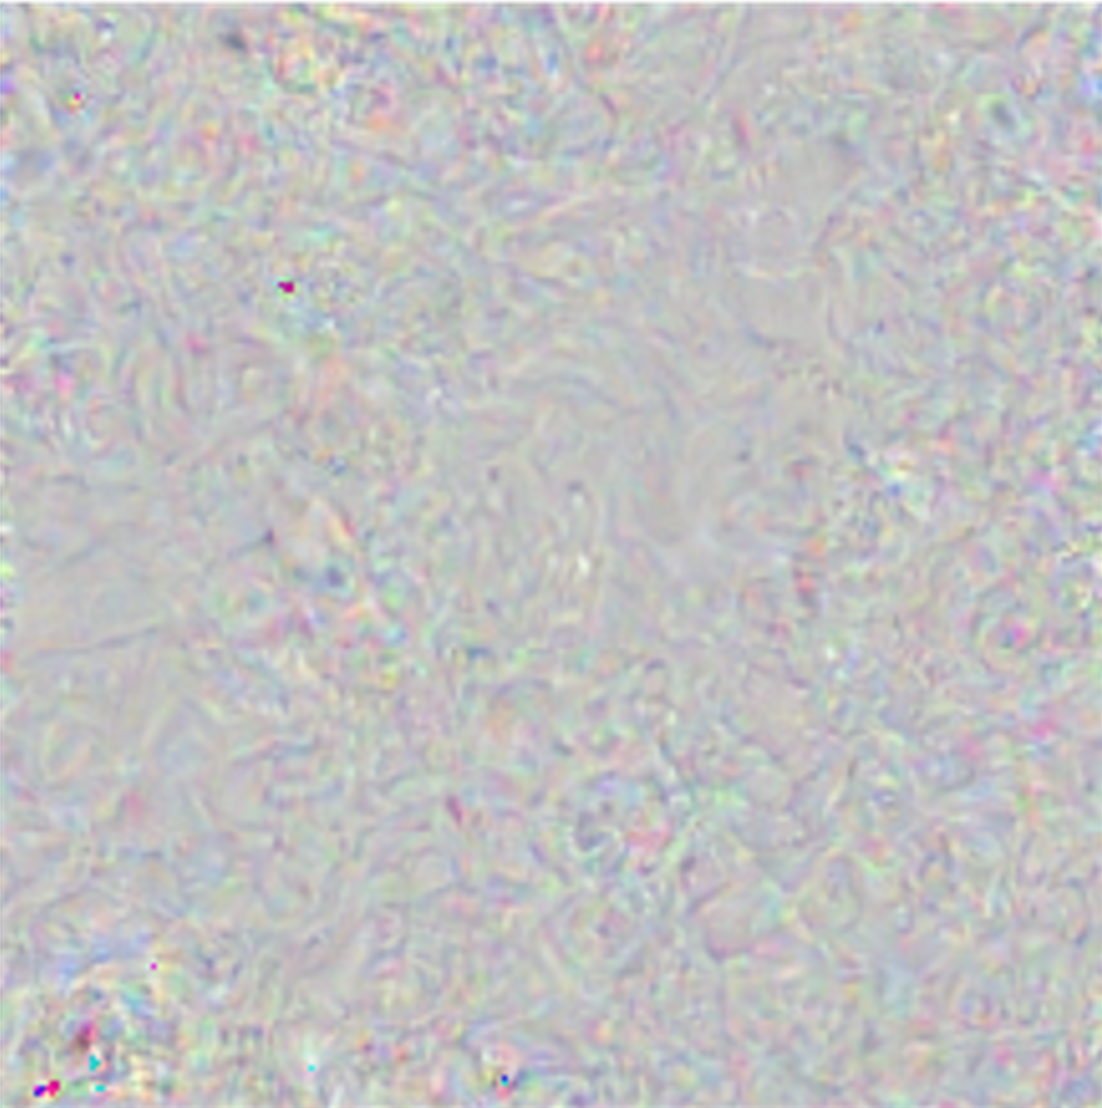
\includegraphics[width=0.6\textwidth]{Images/happy_gradient.png}
    \caption{Generated image maximising happiness}
\end{figure}

Happy posts usually contained pictures of people and in the image gradient we can spot atleast two faces, but that might be because humans are especially good at spotting faces, even when there are none.

\newpage
\section{Generation of text}

We can tweak Deep Sentiment to instead make the neural network generate text by feeding an image. The network will be trained to predict the next word of the text as shown in Figure \ref{deep-prediction}:

\begin{figure}[H]
    \centering
    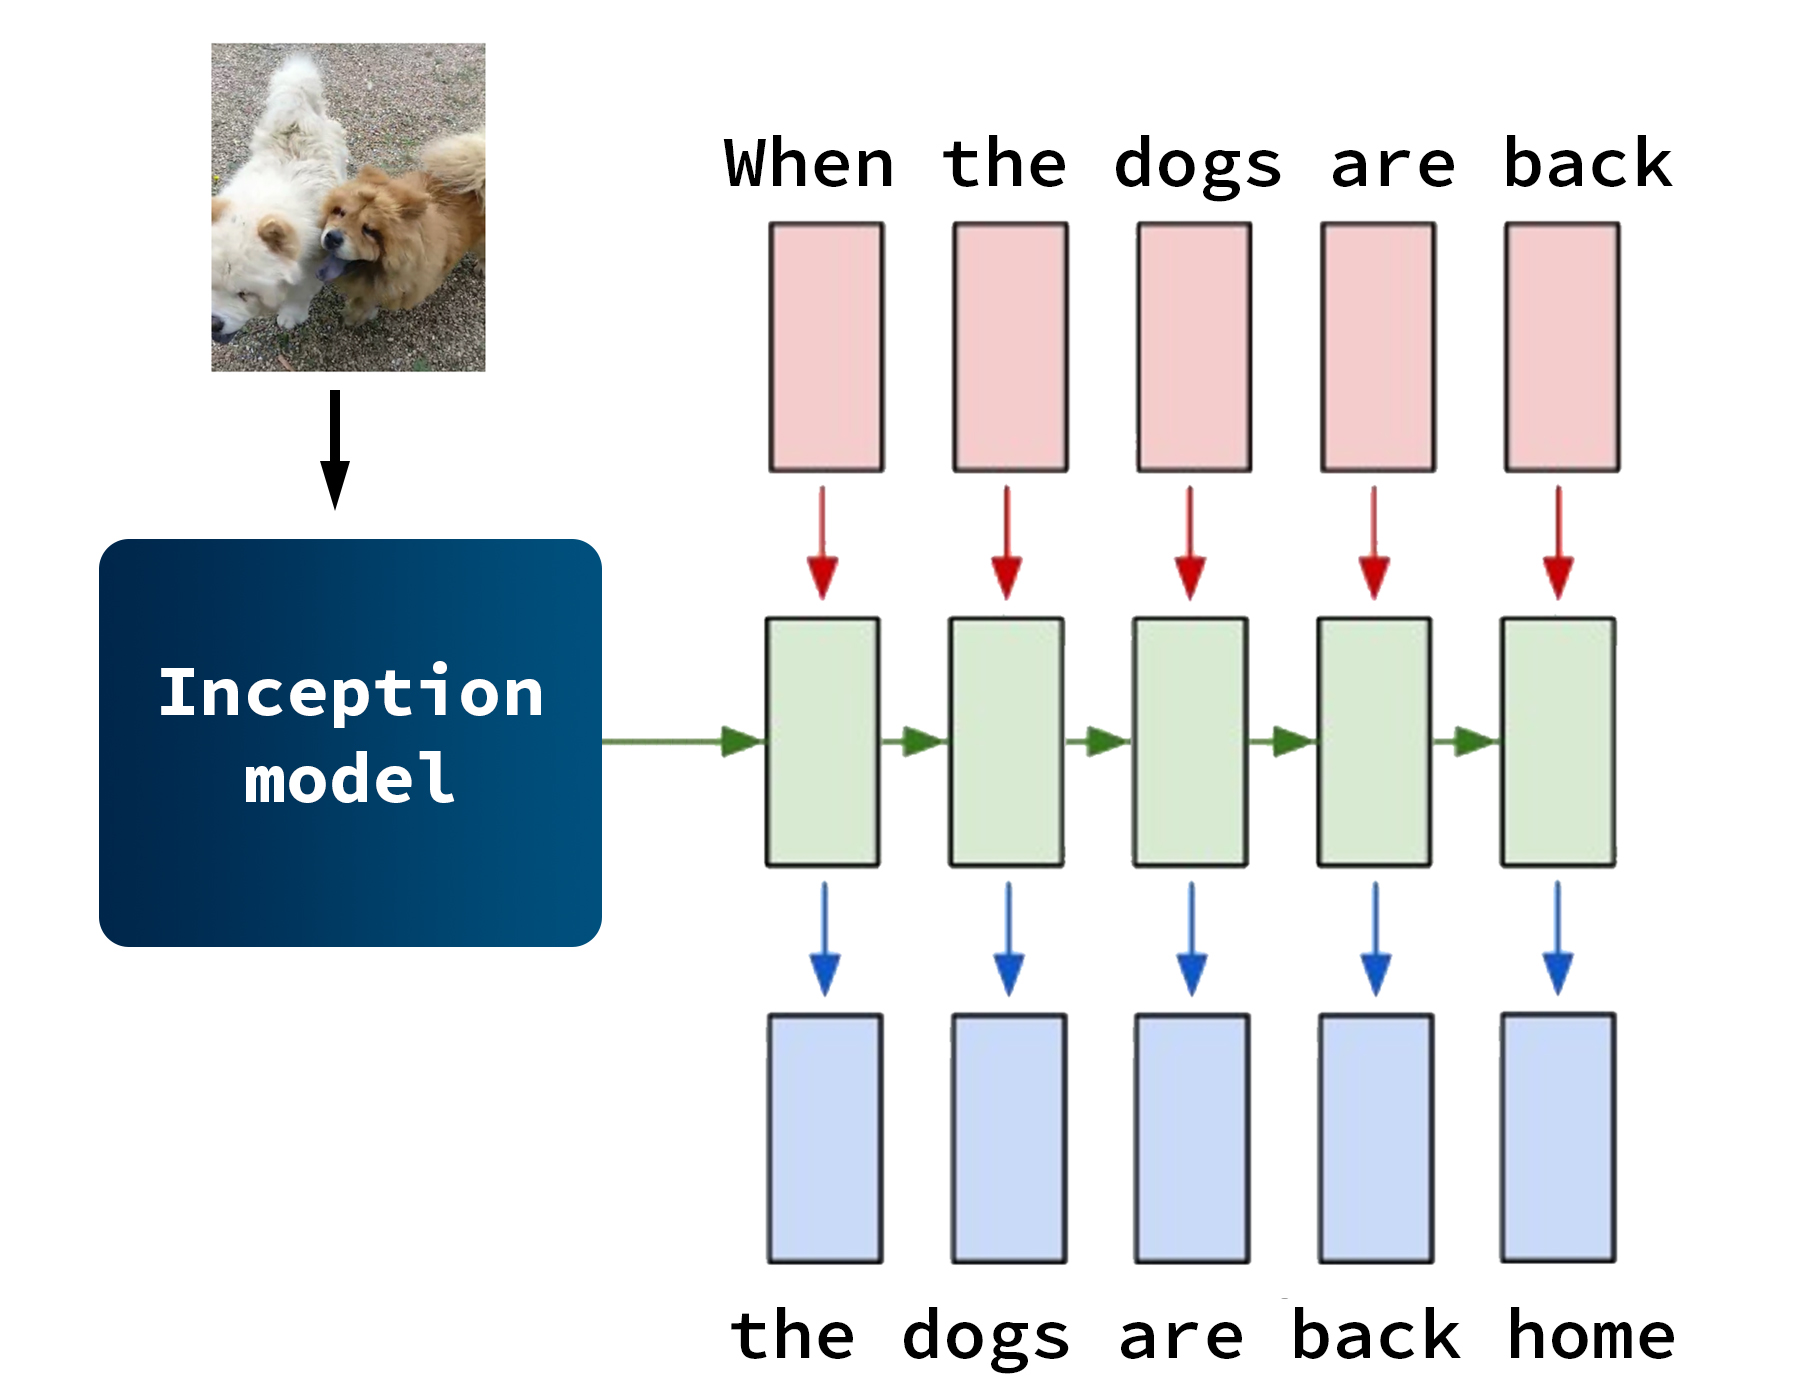
\includegraphics[width=\textwidth]{Images/deep-prediction.jpg}
    \caption{Deep Sentiment for text generation}
    \label{deep-prediction}
\end{figure}

Need to add word embedding in graph

The input words are embedded with Word2Vec and then fed to a one layer LSTM with 512 neurons. The initial hidden state $h_0$ of the LSTM is the output of the Inception network. If we denote by $C$ the number of emotions, the loss $J_{GEN}$ is the sum of the cross-entropy loss of the different predictions $\hat{y}_1, \hat{y}_2, ..., \hat{y}_T \in [0,1]^C$ of the true labels $y_1, y_2, ..., y_T \in \{0, 1\}^C$ (one-hot encoding):
\begin{equation}
    J_{GEN} = \sum_{t=1}^T \text{cross\,entropy}(y_t, \hat{y}_t)
\end{equation}

with the cross-entropy loss given by: $\text{cross\,entropy}(y_t, \hat{y}_t) = -y_t\text{log}(\hat{y}_t)$, therefore:
\begin{equation}
    J_{GEN} = -\sum_{t=1}^T y_t\text{log}(\hat{y}_t)
\end{equation}

The network was trained using only `happy' posts. In order to make batches, each post had a fixed length of 50 words (shorter posts were filled with a special token).

For generation, the network was fed with an image and a random first word in the dictionary. The output would then be a probability distribution of the next word that we would sample from and feed again to the network.

Here is an example of a generated post using this image (which was not in the training set:
\begin{figure}[H]
    \centering
    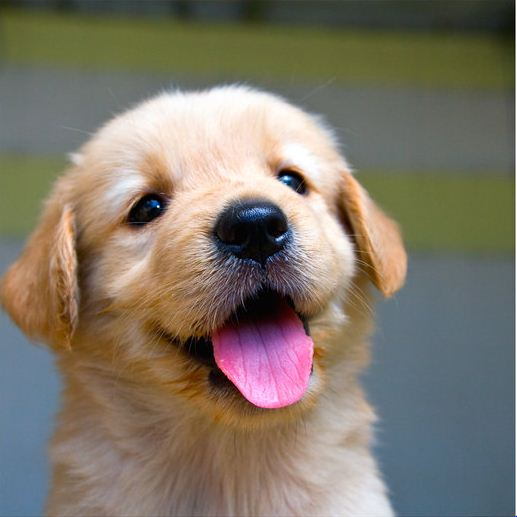
\includegraphics[width=0.3\textwidth]{Images/puppy.jpg}
    \caption{Image used to generate text}
\end{figure}

\begin{quote}
    \textit{Need that just can have a relax months and my perfect film ! \#goodlife \#chill \#fashion}.
\end{quote}

That wouldn't be something a puppy would necessary say but it sounds almost human-like. There are some grammar mistakes such as `a relax months' and unrelated hashtags `\#fashion' but the Tumblr spirit is there.









%\chapter{Generation of Tumblr Posts}

This chapter will be about image and text generation.

%%%%%%%%%%%%%%%%%%%%%%%%%%%%%%%%%%%%%%%%%%%%%%%%%%%%%%%%%%%%
%%%%%%%%%%%%%%%%%%%%  NEW SECTION   %%%%%%%%%%%%%%%%%%%%%%%%
%%%%%%%%%%%%%%%%%%%%%%%%%%%%%%%%%%%%%%%%%%%%%%%%%%%%%%%%%%%%
%\section{}







%\chapter{Useful maths in LaTeX}
%%%%%%%%%%%%%%%%%%%%%%%%%%%%%%%%%%%%%%%%%%%%%%%%%%%%%%%%%%%%
%%%%%%%%%%%%%%%%%%%%  NEW SECTION   %%%%%%%%%%%%%%%%%%%%%%%%
%%%%%%%%%%%%%%%%%%%%%%%%%%%%%%%%%%%%%%%%%%%%%%%%%%%%%%%%%%%%
\section{Equations related}

\begin{align} 
\frac{\partial u_{1}}{\partial t}&  = \Delta w_{1} \quad  \text{in}\;\;\Omega,t>0, \label{1a0001a}\\ 
\frac{\partial u_{2}}{\partial t}&  = \Delta w_{2} \quad \text{in}\;\;\Omega,t>0 ,\label{1a0001b}\\
\intertext{where}
w_{1}  &=  \frac{\delta F(u_{1},u_{2})}{\delta u_{1}}, \label{1a0001c}\\
w_{2}  &=  \frac{\delta F(u_{1},u_{2})}{\delta u_{2}},\label{1a0001d}\\ 
F(u_{1},u_{2})   &=   b_1u_1^4- a_1u_1^2+c_1|\nabla u_1|^2 \nonumber\\
   &\quad  + b_2u_2^4-  a_2u_2^2+c_2|\nabla u_2|^2 \nonumber\\
   &\quad  + D \left(u_1+ \sqrt{\frac{a_1}{2b_1}}\right )^2  \left(u_2+
       \sqrt{\frac{a_2}{2b_2}}\right)^2.\label{1a0001e}
\end{align}

\begin{align}
U^n_1=\sum_{i=1}^{J}U_{1,i}^n\eta_i,\quad W^n_1=\sum_{i=1}^{J}W_{1,i}^n\eta_i,\label{5E0001a}\\
U^n_2=\sum_{i=1}^{J}U_{2,i}^n\eta_i,\quad W^n_2=\sum_{i=1}^{J}W_{2,i}^n\eta_i,\label{5E0001b}
\end{align}

We also use the following notation, for $1 \leq q < \infty,$
\begin{align*}
L^{q}(0,T;W^{m,p}(\Omega)):=& \; \left\{ \eta(x,t):\;  \eta(\cdot,t) \in W^{m,p}(\Omega), \int_0^T  \|\eta(\cdot,t)\|_{m,p}^q\; dt < \infty\right \},\\
L^{\infty}(0,T;W^{m,p}(\Omega)):=& \; \left\{ \eta(x,t):
\eta(\cdot,t) \in W^{m,p}(\Omega)
,\; \displaystyle{\operatornamewithlimits{ess\,sup}_{t\in (0,T)}} \|\eta(\cdot,t)\|_{m,p} < \infty\right \},
\end{align*}

Cases
\begin{equation}
|v|_{0,r} \leq C|v|^{1-\mu}_{0,p} \|v\|^\mu_{m,p},\quad \text{ holds for
} 
r\in 
\begin{cases}
        [p,\infty]&  \mbox{ if }  m-\frac{d}{p} > 0,\\
        [p,\infty) &\mbox{ if } m-\frac{d}{p} = 0,\\
        [p,-\frac{d}{ m-d/p}]& \text{ if } m-\frac{d}{p} < 0.
\end{cases}\label{gagliar}
\end{equation}

\section{Writing}

%=====another Lemma==================
\begin{Lem}\label{Lem201}
Let $u,v,\eta \in H^1{(\Omega)}$, $f=u-v$, $g=u^m v^{n-m}$, $m,n=0,1,2,$ and $n-m\geq
0$. Then for $d=1,2,3,$
\begin{align}
\bigg| \int_\Omega f g \eta dx \bigg| &\leq C |u-v|_0\; \|u\|_1^m\; \|v\|_1^{n-m}\; \|\eta\|_1.
\label{2le000}
\end{align}
\end{Lem}
\bproof
Note that using the Cauchy-Schwarz inequality we have
\begin{align*}
|(u)^m v^{n-m}|_{0,p}&\leq
\begin{cases}
|u|_{0,2mp}^m \;|v|_{0,2(n-m)p}^{(n-m)}&\mbox{for}\;\;
 n-m\neq 0,\;\;\mbox{and}\;\; m\neq 0,\\
|u|_{0,mp}^m \;\;\mbox{or}\;\;|v|_{0,(n-m)p}^{(n-m)}&\mbox{for}\;\;
 m= 0,\;\;\mbox{or}\;\; n-m= 0\;\;\mbox{respectively}.\\
\end{cases}
\end{align*}
Noting the  generalise H\"older inequality  and the result above we have
\begin{align*}
\bigg| \int_\Omega f g \eta dx \bigg| 
&\leq |u-v|_0\;|u^m v^{n-m}|_{0,3}\;|\eta|_{0,6},\\
&\leq |u-v|_0\;\;|\eta|_{0,6}
\begin{cases}
|u|_{0,6}^2\;&\mbox{for}\;\;m=2,\\
|u|_{0,6}\;|v|_{0,6} \;&\mbox{for}\;\;m=1,\\
|v|_{0,6}^2 \;&\mbox{for}\;\;m=0,\\
\end{cases}\\
&\leq C |u-v|_0\; \|u\|_1^m\; \|v\|_1^{n-m}\; \|\eta\|_1,
\end{align*}
where we have noted (\ref{gagliar}) to obtain the last inequality.
This ends the proof.\eproof

We consider the problem: \\
({\textbf P}) \quad Find
$\{u_i, w_i\}$  such that $u_i \in
H^1(0,T;(H^1(\Omega))')\cap L^\infty(0,T;H^1(\Omega))$ for $a.e.$\; $t\in(0,T)$, $ w_i \in L^2(0,T;H^1(\Omega))$ 
%\eqlabon 
$$\left \langle\frac{\partial u_{1}}{\partial t},\eta \right\rangle$$















\chapter{Conclusions}

Deep Sentiment infers the emotional state of Tumblr users with high accuracy by combining textual and visual information.

On images, fine-tuning the Inception network managed to extract useful features at a reduced computational cost as convolutional neural networks are known to be tedious to train. On text, projecting words into a high-dimensional space added semantic understanding of the words that could be effectively used in the recurrent layer to capture the meaning of the sentences. 

The synergy between text and image is quite formidable given the jump in accuracy: from about 40-60\% to 90\%. At a larger scale, this algorithm could be applied population wise in order to have a real-time emotion trend during important events for example.

Deep Sentiment can also be rearranged to generate new Tumblr text matching a given emotion. Changing the model to instead accept characters instead of words could make the model better learn the specific way of writing in blogs.

Likewise, we could try to make the model learn to generate an image given a few blog sentences. The network would try to create an image that most closely matches the text it was given.

Lastly, an interesting experiment to make would be to try to manually label Tumblr posts in order to know whether Deep Sentiment beats human performance.



\begin{thebibliography}{999}
\addcontentsline{toc}{chapter}{\numberline{}Bibliography}

\bibitem{tumblr-photos}
{\bf Tumblr photos:}\\
http://fordosjulius.tumblr.com/post/161996729297/just-relax-with-amazing-view-ocean-and\\
http://ybacony.tumblr.com/post/161878010606/on-a-plane-bitchessss-we-about-to-head-out\\
https://little-sleepingkitten.tumblr.com/post/161996340361/its-okay-to-be-upset-its-okay-to-not-always-be\\
http://shydragon327.tumblr.com/post/161929701863/tensions-were-high-this-caturday\\
https://beardytheshank.tumblr.com/post/161087141680/which-tea-peppermint-tea-what-is-your-favorite\\
https://idreamtofflying.tumblr.com/post/161651437343/me-when-i-see-a-couple-expressing-their-affection

\bibitem{gorner}
{\bf Convolution images:} M. Gorner, Tensorflow and Deep Learning without a PhD, Presentation at \textit{Google Cloud Next '17}\\ 
https://docs.google.com/presentation/d/1TVixw6ItiZ8igjp6U17tcgoFrLSaH\\WQmMOwjlgQY9co/pub?slide=id.g1245051c73\_0\_2184\\
The slide on the convolutional neural network was adapted to our architecture.

\bibitem{camb-spark}
{\bf Max pooling:} Cambridge Spark\\
https://cambridgespark.com/content/tutorials/convolutional-neural-networks-with-keras/index.html

\bibitem{alexnet}
A. Krizhevsky, I. Sutskever and G. Hinton, ImageNet Classification with Deep Convolutional
Neural Networks. In \textit{NIPS}, 2012.

\bibitem{googlenet}
C. Szegedy et al., Going deeper with convolutions. In \textit{CVPR}, 2015.

\bibitem{resnet}
K. He et al., Deep Residual Learning for Image Recognition. In \textit{CVPR}, 2016 .

\bibitem{transfer}
A. Karpathy, L. Fei-Fei, J. Johnson, Transfer Learning. In \textit{Stanford CS231n Convolutional Neural Networks for Visual Recognition}, 2016.

\bibitem{arora}
S. Arora et al., Provable Bounds for Learning Some Deep Representations. In \textit{ICML}, 2014. 

\bibitem{inceptionmodule}
Video explaning Inception Module, https://www.youtube.com/watch?v=VxhSouuSZDY.

\bibitem{word2vec}
T. Mikolov et al., Efficient Estimation of Word Representations in Vector Space. In \textit{ICLR}, 2013.

\bibitem{comparison-text}
TensorFlow, Word2Vec tutorial, https://www.tensorflow.org/tutorials/word2vec.

\bibitem{word2vec-architecture}
C. McCormick, Word2Vec Tutorial - The Skip-Gram Model, http://mccormickml.com/2016/04/19/word2vec-tutorial-the-skip-gram-model/.

\bibitem{word2vec2}
T. Mikolov et al., Distributed Representations of Words and Phrases and their Compositionality. In \textit{NIPS}, 2013.

\end{thebibliography}





\appendix
\setcounter{chapter}{0}
% \numberline{} aligns 'Appendix' with the rest of the chapters
\addcontentsline{toc}{chapter}{\numberline{}Appendix}
\chapter{Python Code}
\lstset{language=Python}
\lstset{frame=lines}
\lstset{basicstyle=\scriptsize}
\lstset{showstringspaces=false}

\section{Tumblr Data}

\subsection{Data Extraction}
\begin{lstlisting}
import numpy as np

def extract_tumblr_posts(client, nb_requests, search_query, before, delta_limit):
    """Extract Tumblr posts with a given emotion.
    
    Parameters:
        client: Authenticated Tumblr client with the pytumblr package.
        nb_requests: Number of API request.
        search_query: Emotion to search for.
        before: A timestamp to search for posts before that value.
        delta_limit: Maximum difference of timestamp between two queries.
    """    
    for i in range(nb_requests):
        tagged = client.tagged(search_query, filter='text', before=before)
        nb_rejected = 0
        timestamps_rejected = []
        for elt in tagged:
            timestamp = elt['timestamp']
            if (abs(timestamp - before) < delta_limit):
                before = timestamp

                current_post = []
                current_post.append(elt['id'])
                current_post.append(elt['post_url'])

                elt_type = elt['type']
                current_post.append(elt_type)
                current_post.append(timestamp)
                current_post.append(elt['date'])
                current_post.append(elt['tags'])
                current_post.append(elt['liked'])
                current_post.append(elt['note_count'])

                if (elt_type == 'photo'):
                    # Only take the first image
                    current_post.append(elt['photos'][0]['original_size']['url'])
                    current_post.append(elt['caption'].replace('\n',' ').replace('\r',' '))
                    current_post.append(search_query)
                    posts.append(current_post)
                elif (elt_type == 'text'):
                    current_post.append(np.nan)
                    current_post.append(elt['body'].replace('\n',' ').replace('\r',' '))
                    current_post.append(search_query)
                    posts.append(current_post)
            else:
                nb_rejected += 1
                timestamps_rejected.append(timestamp)

            return (posts, nb_rejected, timestamps_rejected)
\end{lstlisting}

\subsection{Data Preprocessing and Conversion for TensorFlow}
\begin{lstlisting}
import os
import urllib2
import io
import random
import sys
import math

import pandas as pd
import tensorflow as tf

from PIL import Image
from scipy.misc import imread, imresize
from slim.nets import inception
from datasets import dataset_utils
from text_model.text_preprocessing import preprocess_one_df
from text_model.text_preprocessing import _load_embedding_weights_glove

def download_im_with_text(search_query, start, end, dataset_dir='data', subdir='photos'):
    """Download images using the urls in the dataframe specified by the search query.

    Parameters:
        search_query: A string giving the sentiment to load the corresponding dataframe.
        start: A start index for the loaded dataframe.
        end: An end index for the loaded dataframe.
        dataset_dir: A directory where the dataframes are stored.
        subdir: A subdirectory to store the photos.

    Returns:
        Images downloaded in the directory dataset_dir/subdir/search_query, having 
        the posts ids as names.
    """
    # Load data
    emb_name = 'glove'
    text_dir = 'text_model'
    emb_dir = 'embedding_weights'
    filename = 'glove.6B.50d.txt'
    if emb_name == 'word2vec':
        vocabulary, embedding = _load_embedding_weights_word2vec(text_dir, emb_dir, filename)
    else:
        vocabulary, embedding = _load_embedding_weights_glove(text_dir, emb_dir, filename)

    df = preprocess_one_df(vocabulary, embedding, search_query, _POST_SIZE)
    links = df['photo']
    # Create subdir if it doesn't exist
    if not tf.gfile.Exists(os.path.join(dataset_dir, subdir)):
        tf.gfile.MakeDirs(os.path.join(dataset_dir, subdir))
    # Create search_query folder if it doesn't exist
    photos_dir = os.path.join(dataset_dir, subdir, search_query)
    if not tf.gfile.Exists(photos_dir):
        tf.gfile.MakeDirs(photos_dir)
    for i in range(start, end):
        # Check for NaNs
        if links[i] == links[i]:
            # Open url and convert to JPEG image
            try:
                f = urllib2.urlopen(links[i])
            except Exception:
                continue
            image_file = io.BytesIO(f.read())
            im = Image.open(image_file)
            # The filename is the index of the image in the dataframe
            filename = str(i) + '.jpg'
            im.convert('RGB').save(os.path.join(photos_dir, filename), 'JPEG')
            
%convert to tfrecords
def convert_images_with_text(dataset_dir, num_valid, photos_subdir='photos', 
    tfrecords_subdir='tfrecords'):
    """Downloads the photos and convert them to TFRecords.

    Parameters:
        dataset_dir: The data directory.
        photos_subdir: The subdirectory where the photos are stored.
        tfrecords_subdir: The subdirectory to store the TFRecords files.
    """
    # Create the tfrecords_subdir if it doesn't exist
    if not tf.gfile.Exists(os.path.join(dataset_dir, tfrecords_subdir)):
        tf.gfile.MakeDirs(os.path.join(dataset_dir, tfrecords_subdir))

    if _dataset_exists(dataset_dir, photos_subdir):
        print('Dataset files already exist. Exiting without re-creating them.')
        return

    photo_filenames, class_names = _get_filenames_and_classes(dataset_dir, photos_subdir)
    class_names_to_ids = dict(zip(class_names, range(len(class_names))))

    # Divide into train and test:
    random.seed(_RANDOM_SEED)
    random.shuffle(photo_filenames)
    training_filenames = photo_filenames[num_valid:]
    validation_filenames = photo_filenames[:num_valid]

    # Load dataframes
    df_dict = dict()
    emotions = ['happy', 'sad', 'scared', 'angry', 'surprised', 'disgusted']
    emb_name = 'glove'
    text_dir = 'text_model'
    emb_dir = 'embedding_weights'
    filename = 'glove.6B.50d.txt'
    if emb_name == 'word2vec':
        vocabulary, embedding = _load_embedding_weights_word2vec(text_dir, emb_dir, filename)
    else:
        vocabulary, embedding = _load_embedding_weights_glove(text_dir, emb_dir, filename)

    for emotion in emotions:
        df_dict[emotion] = preprocess_one_df(vocabulary, embedding, emotion, _POST_SIZE)

    # First, convert the training and validation sets.
    _convert_dataset_with_text('train', training_filenames, class_names_to_ids,
                               dataset_dir, df_dict, tfrecords_subdir)
    _convert_dataset_with_text('validation', validation_filenames, class_names_to_ids,
                               dataset_dir, df_dict, tfrecords_subdir)

    # Write the train/validation split size
    train_valid_split = dict(zip(['train', 'validation'], [len(photo_filenames) - num_valid, 
        num_valid]))
    train_valid_filename = os.path.join(dataset_dir, photos_subdir, _TRAIN_VALID_FILENAME)
    with tf.gfile.Open(train_valid_filename, 'w') as f:
        for split_name in train_valid_split:
            size = train_valid_split[split_name]
            f.write('%s:%d\n' % (split_name, size))

    # Finally, write the labels file:
    labels_to_class_names = dict(zip(range(len(class_names)), class_names))
    dataset_utils.write_label_file(labels_to_class_names, dataset_dir, photos_subdir)

    #_clean_up_temporary_files(dataset_dir)
    print('\nFinished converting the dataset!')
    
%get_split
def get_split_with_text(split_name, dataset_dir, photos_subdir='photos', 
  tfrecords_subdir='tfrecords', file_pattern=None, reader=None):
    """Gets a dataset tuple with instructions for reading tumblr data.

    Args:
        split_name: A train/validation split name.
        dataset_dir: The base directory of the dataset sources.
        photos_subdir: The subdirectory containing the photos.
        tfrecords_subdir: The subdirectory containing the TFRecords files.
        file_pattern: The file pattern to use when matching the dataset sources.
            It is assumed that the pattern contains a '%s' string so that the split
            name can be inserted.
        reader: The TensorFlow reader type.

    Returns:
        A `Dataset` namedtuple.

    Raises:
        ValueError: if `split_name` is not a valid train/validation split.
    """
    #if split_name not in SPLITS_TO_SIZES:
        #raise ValueError('split name %s was not recognized.' % split_name)

    if not file_pattern:
        file_pattern = _FILE_PATTERN
    file_pattern = os.path.join(dataset_dir, tfrecords_subdir, file_pattern % split_name)

    # Allowing None in the signature so that dataset_factory can use the default.
    if reader is None:
        reader = tf.TFRecordReader

    keys_to_features = {
      'image/encoded': tf.FixedLenFeature((), tf.string, default_value=''),
      'image/format': tf.FixedLenFeature((), tf.string, default_value='jpg'),
      'image/class/label': tf.FixedLenFeature(
          [], tf.int64, default_value=tf.zeros([], dtype=tf.int64)),
      'text': tf.FixedLenFeature(
          [_POST_SIZE], tf.int64, default_value=tf.zeros([_POST_SIZE], dtype=tf.int64)),
    }

    items_to_handlers = {
      'image': slim.tfexample_decoder.Image(),
      'text': slim.tfexample_decoder.Tensor('text'),
      'label': slim.tfexample_decoder.Tensor('image/class/label'),
    }

    decoder = slim.tfexample_decoder.TFExampleDecoder(
        keys_to_features, items_to_handlers)

    labels_to_names = None
    if dataset_utils.has_labels(dataset_dir, photos_subdir):
        labels_to_names = dataset_utils.read_label_file(dataset_dir, photos_subdir)

    # Get split size
    train_valid_filename = os.path.join(dataset_dir, photos_subdir, _TRAIN_VALID_FILENAME)
    with tf.gfile.Open(train_valid_filename, 'rb') as f:
        lines = f.read().decode()
    lines = lines.split('\n')
    lines = filter(None, lines)

    train_valid_split = {}
    for line in lines:
        index = line.index(':')
        train_valid_split[line[:index]] = (int)(line[index+1:])

    return slim.dataset.Dataset(
      data_sources=file_pattern,
      reader=reader,
      decoder=decoder,
      num_samples=train_valid_split[split_name],
      items_to_descriptions=_ITEMS_TO_DESCRIPTIONS,
      num_classes=len(labels_to_names),
      labels_to_names=labels_to_names)
\end{lstlisting}

\newpage
\section{Visual Recognition}
\begin{lstlisting}
""" Fine-tune a pre-trained Inception model by chopping off the last logits layer. 
"""
import os
import sys

import numpy as np
import tensorflow as tf

from tensorflow.contrib import slim
from tensorflow.contrib.slim.python.slim.learning import train_step
from sklearn.linear_model import LogisticRegression
from sklearn.ensemble import RandomForestClassifier
from sklearn.metrics import accuracy_score

from slim.preprocessing import inception_preprocessing
#from slim.nets import inception
from image_model import inception_v1
from datasets import dataset_utils
from datasets.convert_to_dataset import get_split, get_split_with_text
from datasets.convert_images_tfrecords import get_numpy_data

# Seed for reproducibility
_RANDOM_SEED = 0

def download_pretrained_model(url, checkpoint_dir):
    """Download pretrained inception model and store it in checkpoint_dir.

    Parameters:
        url: The url containing the compressed model.
        checkpoint_dir: The directory to save the model.
    """
    if not tf.gfile.Exists(checkpoint_dir):
        tf.gfile.MakeDirs(checkpoint_dir)
    dataset_utils.download_and_uncompress_tarball(url, checkpoint_dir)

def _load_batch(dataset, batch_size=32, shuffle=True, height=299, width=299, 
    is_training=False):
    """Load a single batch of data. 
    
    Args:
      dataset: The dataset to load.
      batch_size: The number of images in the batch.
      shuffle: Whether to shuffle the data sources and common queue when reading.
      height: The size of each image after preprocessing.
      width: The size of each image after preprocessing.
      is_training: Whether or not we're currently training or evaluating.
    
    Returns:
      images: A Tensor of size [batch_size, height, width, 3], image samples that have 
          been preprocessed.
      images_raw: A Tensor of size [batch_size, height, width, 3], image samples that 
                           can be used for visualization.
      labels: A Tensor of size [batch_size], whose values range between 0 and dataset.num_classes.
    """
    # For validation, if you set the common_queue_capacity to something lower than
    # batch_size, which is the validation size, then your output will contain duplicates.
    data_provider = slim.dataset_data_provider.DatasetDataProvider(
        dataset, shuffle=shuffle, common_queue_capacity=batch_size,
        common_queue_min=8)
    image_raw, label = data_provider.get(['image', 'label'])
    
    # Preprocess image for usage by Inception.
    image = inception_preprocessing.preprocess_image(image_raw, height, width, 
        is_training=is_training)

    # Preprocess the image for display purposes.
    image_raw = tf.expand_dims(image_raw, 0)
    image_raw = tf.image.resize_images(image_raw, [height, width])
    image_raw = tf.squeeze(image_raw)

    # Batch it up.
    images, images_raw, labels = tf.train.batch(
        [image, image_raw, label],
        batch_size=batch_size,
        num_threads=1,
        capacity=2 * batch_size)
    
    return images, images_raw, labels

def load_batch_with_text(dataset, batch_size=32, shuffle=True, height=299, width=299, 
    is_training=False):
    """Load a single batch of data. 
    
    Args:
      dataset: The dataset to load.
      batch_size: The number of images in the batch.
      shuffle: Whether to shuffle the data sources and common queue when reading.
      height: The size of each image after preprocessing.
      width: The size of each image after preprocessing.
      is_training: Whether or not we're currently training or evaluating.
    
    Returns:
      images: A Tensor of size [batch_size, height, width, 3], image samples that have been 
          preprocessed.
      images_raw: A Tensor of size [batch_size, height, width, 3], image samples that can 
          be used for visualization.
      labels: A Tensor of size [batch_size], whose values range between 0 and dataset.num_classes.
    """
    # For validation, if you set the common_queue_capacity to something lower than
    # batch_size, which is the validation size, then your output will contain duplicates.
    data_provider = slim.dataset_data_provider.DatasetDataProvider(
        dataset, shuffle=shuffle, common_queue_capacity=batch_size,
        common_queue_min=8)
    image_raw, text, label = data_provider.get(['image', 'text', 'label'])
    
    # Preprocess image for usage by Inception.
    image = inception_preprocessing.preprocess_image(image_raw, height, width, 
        is_training=is_training)

    # Preprocess the image for display purposes.
    image_raw = tf.expand_dims(image_raw, 0)
    image_raw = tf.image.resize_images(image_raw, [height, width])
    image_raw = tf.squeeze(image_raw)

    # Batch it up.
    images, images_raw, texts, labels = tf.train.batch(
        [image, image_raw, text, label],
        batch_size=batch_size,
        num_threads=1,
        capacity=2 * batch_size)
    
    return images, images_raw, texts, labels

def get_init_fn(checkpoints_dir, model_name='inception_v1.ckpt'):
    """Returns a function run by the chief worker to warm-start the training.
    """
    checkpoint_exclude_scopes=["InceptionV1/Logits", "InceptionV1/AuxLogits"]
    
    exclusions = [scope.strip() for scope in checkpoint_exclude_scopes]

    variables_to_restore = []
    for var in slim.get_model_variables():
        excluded = False
        for exclusion in exclusions:
            if var.op.name.startswith(exclusion):
                excluded = True
                break
        if not excluded:
            variables_to_restore.append(var)

    return slim.assign_from_checkpoint_fn(
        os.path.join(checkpoints_dir, model_name),
        variables_to_restore)

def fine_tune_model(dataset_dir, checkpoints_dir, train_dir, num_steps):
    """Fine tune the inception model, retraining the last layer.

    Parameters:
        dataset_dir: The directory containing the data.
        checkpoints_dir: The directory contained the pre-trained model.
        train_dir: The directory to save the trained model.
        num_steps: The number of steps training the model.
    """
    if tf.gfile.Exists(train_dir):
        # Delete old model
        tf.gfile.DeleteRecursively(train_dir)
    tf.gfile.MakeDirs(train_dir)

    with tf.Graph().as_default():
        tf.logging.set_verbosity(tf.logging.INFO)
        
        dataset = get_split('train', dataset_dir)
        image_size = inception_v1.default_image_size
        images, _, labels = _load_batch(dataset, height=image_size, width=image_size)

        # Load validation data
        dataset_valid = get_split('validation', dataset_dir)
        images_valid, _, labels_valid = _load_batch(dataset_valid, 
            batch_size=dataset_valid.num_samples, 
            shuffle=False, height=image_size, width=image_size)
        
        # Create the model, use the default arg scope to configure the batch norm parameters.
        with slim.arg_scope(inception_v1.inception_v1_arg_scope()):
            logits, _ = inception_v1.inception_v1(images, num_classes=dataset.num_classes, 
                is_training=True)
            logits_valid, _ = inception_v1.inception_v1(images_valid, 
                num_classes=dataset_valid.num_classes, is_training=False, reuse=True)
            
        # Specify the loss function:
        one_hot_labels = slim.one_hot_encoding(labels, dataset.num_classes)
        slim.losses.softmax_cross_entropy(logits, one_hot_labels)
        total_loss = slim.losses.get_total_loss()

        # Create some summaries to visualize the training process:
        tf.summary.scalar('losses/Total_Loss', total_loss)
      
        # Specify the optimizer and create the train op:
        optimizer = tf.train.AdamOptimizer(learning_rate=1e-5)
        train_op = slim.learning.create_train_op(total_loss, optimizer)

        # Accuracy metrics
        accuracy_valid = slim.metrics.accuracy(tf.cast(labels_valid, tf.int32),
                                               tf.cast(tf.argmax(logits_valid, 1), tf.int32))

        def train_step_fn(session, *args, **kwargs):
            total_loss, should_stop = train_step(session, *args, **kwargs)
            acc_valid = session.run(accuracy_valid)
            sys.stdout.flush()
            train_step_fn.step += 1
            return [total_loss, should_stop]
        
        train_step_fn.step = 0

        # Run the training:
        final_loss = slim.learning.train(
            train_op,
            logdir=train_dir,
            init_fn=get_init_fn(checkpoints_dir),
            train_step_fn=train_step_fn,
            number_of_steps=num_steps)
            
    print('Finished training. Last batch loss {0:.3f}'.format(final_loss))

def fine_tune_model_with_text(dataset_dir, checkpoints_dir, train_dir, num_steps, 
    learning_rate):
    """Fine tune the inception model, retraining the last layer.

    Parameters:
        dataset_dir: The directory containing the data.
        checkpoints_dir: The directory contained the pre-trained model.
        train_dir: The directory to save the trained model.
        num_steps: The number of steps training the model.
    """
    if tf.gfile.Exists(train_dir):
        # Delete old model
        tf.gfile.DeleteRecursively(train_dir)
    tf.gfile.MakeDirs(train_dir)

    with tf.Graph().as_default():
        tf.logging.set_verbosity(tf.logging.INFO)
        
        dataset = get_split_with_text('train', dataset_dir)
        image_size = inception_v1.default_image_size
        images, _, labels = _load_batch(dataset, height=image_size, width=image_size)
        
        # Create the model, use the default arg scope to configure the batch norm parameters.
        with slim.arg_scope(inception_v1.inception_v1_arg_scope()):
            logits, _ = inception_v1.inception_v1(images, num_classes=dataset.num_classes, 
                is_training=True)
            
        # Specify the loss function:
        one_hot_labels = slim.one_hot_encoding(labels, dataset.num_classes)
        slim.losses.softmax_cross_entropy(logits, one_hot_labels)
        total_loss = slim.losses.get_total_loss()

        # Create some summaries to visualize the training process
        # Use tensorboard --logdir=train_dir, careful with pat
        # Different from the logs, because computed on different mini batch of data
        tf.summary.scalar('Loss', total_loss)
      
        # Specify the optimizer and create the train op:
        optimizer = tf.train.AdamOptimizer(learning_rate=learning_rate)
        train_op = slim.learning.create_train_op(total_loss, optimizer)

        def train_step_fn(session, *args, **kwargs):
            total_loss, should_stop = train_step(session, *args, **kwargs)
            #acc_valid = session.run(accuracy_valid)
            sys.stdout.flush()
            train_step_fn.step += 1
            return [total_loss, should_stop]
        
        train_step_fn.step = 0

        # Run the training:
        final_loss = slim.learning.train(
            train_op,
            logdir=train_dir,
            init_fn=get_init_fn(checkpoints_dir),
            save_interval_secs=60,
            save_summaries_secs=60,
            #train_step_fn=train_step_fn,
            number_of_steps=num_steps)
            
    print('Finished training. Last batch loss {0:.3f}'.format(final_loss))

def evaluate_model(checkpoint_dir, log_dir, num_evals):
    """Visualise results with: tensorboard --logdir=logdir.
    
    Parameters:
        checkpoint_dir: Checkpoint of the saved model during training.
        log_dir: Directory to save logs.
        num_evals: Number of batches to evaluate (mean of the batches is displayed).
    """
    
    with tf.Graph().as_default():
        tf.logging.set_verbosity(tf.logging.INFO)

        dataset_dir = 'data'
        # Load train data
        image_size = inception_v1.default_image_size

        dataset_train = get_split_with_text('train', dataset_dir)
        images_train, _, labels_train = _load_batch(dataset_train, batch_size=32, shuffle=False, 
                                                    height=image_size, width=image_size)

        # Create the model, use the default arg scope to configure the batch norm parameters.
        with slim.arg_scope(inception_v1.inception_v1_arg_scope()):
            logits_train, _ = inception_v1.inception_v1(images_train, 
                num_classes=dataset_train.num_classes, 
                                                        is_training=False, reuse=True)
        # Accuracy metrics
        accuracy_train = slim.metrics.streaming_accuracy(tf.cast(labels_train, tf.int32),
            tf.cast(tf.argmax(logits_train, 1), tf.int32))

        # Load validation data
        dataset_valid = get_split_with_text('validation', dataset_dir)
        images_valid, _, labels_valid = _load_batch(dataset_valid, batch_size=32, shuffle=False, 
            height=image_size, width=image_size)

        # Create the model, use the default arg scope to configure the batch norm parameters.
        with slim.arg_scope(inception_v1.inception_v1_arg_scope()):
            logits_valid, _ = inception_v1.inception_v1(images_valid, 
                num_classes=dataset_valid.num_classes, 
                                                        is_training=False, reuse=True)
        # Accuracy metrics
        accuracy_valid = slim.metrics.streaming_accuracy(tf.cast(labels_valid, tf.int32), 
            tf.cast(tf.argmax(logits_valid, 1), tf.int32))

        # Choose the metrics to compute:
        names_to_values, names_to_updates = slim.metrics.aggregate_metric_map({
            'accuracy_train': accuracy_train,
            'accuracy_valid': accuracy_valid,
        })

        for metric_name, metric_value in names_to_values.iteritems():
            tf.summary.scalar(metric_name, metric_value)

        # Evaluate every eval_interval_secs secs or if not specified,
        # every time the checkpoint_dir changes
        slim.evaluation.evaluation_loop(
            '',
            checkpoint_dir,
            log_dir,
            num_evals=num_evals,
            eval_op=names_to_updates.values())

def evaluate_model_2(checkpoint_dir, log_dir, mode, num_evals):
    """Visualise results with: tensorboard --logdir=logdir. 
    
    Parameters:
        checkpoint_dir: Checkpoint of the saved model during training.
        log_dir: Directory to save logs.
        mode: train or validation.
        num_evals: Number of batches to evaluate (mean of the batches is displayed).
    """
    
    with tf.Graph().as_default():
        tf.logging.set_verbosity(tf.logging.INFO)

        dataset_dir = 'data'
        # Load train data
        image_size = inception_v1.default_image_size

        dataset = get_split_with_text(mode, dataset_dir)
        images, _, labels = _load_batch(dataset, batch_size=32, shuffle=False, 
                                        height=image_size, width=image_size)

        # Create the model, use the default arg scope to configure the batch norm parameters.
        with slim.arg_scope(inception_v1.inception_v1_arg_scope()):
            logits, _ = inception_v1.inception_v1(images, num_classes=dataset.num_classes, 
                                                  is_training=False, reuse=True)
        # Accuracy metrics
        accuracy = slim.metrics.streaming_accuracy(tf.cast(labels, tf.int32),
                                                   tf.cast(tf.argmax(logits, 1), tf.int32))

        # Choose the metrics to compute:
        names_to_values, names_to_updates = slim.metrics.aggregate_metric_map({
            'accuracy': accuracy,
        })

        for metric_name, metric_value in names_to_values.iteritems():
            tf.summary.scalar(metric_name, metric_value)

        log_dir = os.path.join(log_dir, mode)

        # Evaluate every eval_interval_secs secs or if not specified,
        # every time the checkpoint_dir changes
        slim.evaluation.evaluation_loop(
            '',
            checkpoint_dir,
            log_dir,
            num_evals=num_evals,
            eval_op=names_to_updates.values())
        
def softmax_regression(num_valid, C):
    """Run a softmax regression on the images.

    Parameters:
        num_valid: Size of the validation set.
        C: Inverse of the regularization strength.
    """
    # Load data
    X_train, X_valid, y_train, y_valid = get_numpy_data('data', num_valid)
    logistic = LogisticRegression(multi_class='multinomial', solver='newton-cg',
                                  C=C, random_state=_RANDOM_SEED)
    print('Start training Logistic Regression.')
    logistic.fit(X_train, y_train)

    accuracy_train = accuracy_score(logistic.predict(X_train), y_train)
    valid_accuracy = accuracy_score(logistic.predict(X_valid), y_valid)
    print('Training accuracy: {0:.3f}'.format(accuracy_train))
    print('Validation accuracy: {0:.3f}'.format(valid_accuracy))

def forest(num_valid, n_estimators, max_depth):
    """Run a Random Forest on the images.

    Parameters:
        num_valid: Size of the validation set.
        n_estimators: Number of trees.
        max_depth: Maximum depth of a tree.
    """
    # Load data
    X_train, X_valid, y_train, y_valid = get_numpy_data('data', num_valid)
    forest = RandomForestClassifier(n_estimators=n_estimators, max_depth=max_depth, 
                                    random_state=_RANDOM_SEED)
    print('Start training Random Forest.')
    forest.fit(X_train, y_train)

    accuracy_train = accuracy_score(forest.predict(X_train), y_train)
    valid_accuracy = accuracy_score(forest.predict(X_valid), y_valid)
    print('Training accuracy: {0:.3f}'.format(accuracy_train))
    print('Validation accuracy: {0:.3f}'.format(valid_accuracy))
\end{lstlisting}

\newpage
\section{Natural Language Processing}

\subsection{Text Preprocessing}
\begin{lstlisting}
import os
import re
import gensim

import numpy as np
import pandas as pd

# string.punctuation
_PUNCTUATION = u'!"$%&\'()*+,./:;<=>?[\\]^_`{|}~#'

_MIN_ENGLISH_WORDS_IN_POST = 5

def _load_embedding_weights_glove(text_dir, emb_dir, filename):
    """Load the word embedding weights from a pre-trained model.
    
    Parameters:
        text_dir: The directory containing the text model.
        emb_dir: The subdirectory containing the weights.
        filename: The name of that text file.
        
    Returns:
        vocabulary: A list containing the words in the vocabulary.
        embedding: A numpy array of the weights.
    """
    vocabulary = []
    embedding = []
    with open(os.path.join(text_dir, emb_dir, filename), 'rb') as f:
        for line in f.readlines():
            row = line.strip().split(' ')
            # Convert to unicode
            vocabulary.append(row[0].decode('utf-8', 'ignore'))
            embedding.append(map(np.float32, row[1:]))
        embedding = np.array(embedding)
        print('Finished loading word embedding weights.')
    return vocabulary, embedding

def _load_embedding_weights_word2vec(text_dir, emb_dir, filename):
    """Load the word embedding weights from a pre-trained model.
    
    Parameters:
        text_dir: The directory containing the text model.
        emb_dir: The subdirectory containing the weights.
        filename: The name of the binary file.
        
    Returns:
        vocabulary: A list containing the words in the vocabulary.
        embedding: A numpy array of the weights.
    """
    word2vec_dir = os.path.join(text_dir, emb_dir, filename)
    model = gensim.models.KeyedVectors.load_word2vec_format(word2vec_dir, binary=True)
    vocabulary = model.index2word
    embedding = model.syn0
    print('Finished loading word embedding weights.')
    return vocabulary, embedding

def _str_list_to_set(str_list):
    """Convert a string representation of a list such as '[happy, sun, outdoors]'
       to a set of strings {'happy', 'sun', 'outdoors'}
    """
    output = str_list[1:-1].split(',')
    output = set([x.strip() for x in output])
    return output

def _df_with_hashtag_in_post(df, tag):
    """Make sure that the relevant hashtag is in the post.
    """
    df['tags'] = df['tags'].map(_str_list_to_set)
    mask = df['tags'].map(lambda x: tag in x)
    return df.loc[mask, :].reset_index(drop=True)

def _is_valid_text(paragraph, vocab_set):
    """Check that a post contains atleast _MIN_ENGLISH_WORDS_IN_POST words in english.
    """
    # Check for nan text
    if (type(paragraph) == float) and (np.isnan(paragraph)):
        return False
    else:
        regex = re.compile('[%s]' % re.escape(_PUNCTUATION))
        # Remove punctuation, convert to lower case before splitting
        words = regex.sub('', paragraph).lower().split()
        # Check if there are atleast _MIN_ENGLISH_WORDS_IN_POST words in english
        return len(set(words).intersection(vocab_set)) > _MIN_ENGLISH_WORDS_IN_POST

def _paragraph_to_ids(paragraph, word_to_id, post_size, emotions):
    """Convert a paragraph to a list of ids, removing the #emotion.
    """
    words = []
    vocab_size = len(word_to_id)

    # Remove emotion hashtags from the post.
    emotion_regex = re.compile('|'.join(map(re.escape, ['#' + emotion for emotion in emotions])))
    paragraph = emotion_regex.sub('', paragraph.lower())

    regex = re.compile('[%s]' % re.escape(_PUNCTUATION))
    # Remove punctuation, convert to lower case before splitting
    words = regex.sub('', paragraph).lower().split()
    # Replace unknown words by an id equal to the size of the vocab
    words = map(lambda x: word_to_id.get(x, vocab_size), words)
        
    if len(words) > post_size:
        words = words[:post_size]
    else:
        words = words + [vocab_size] * (post_size - len(words))
    return words

def preprocess_df(text_dir, emb_dir, filename, emb_name, emotions, post_size):
    """Preprocess emotion dataframes.
    """
    if emb_name == 'word2vec':
        vocabulary, embedding = _load_embedding_weights_word2vec(text_dir, emb_dir, filename)
    else:
        vocabulary, embedding = _load_embedding_weights_glove(text_dir, emb_dir, filename)
    vocab_size, embedding_dim = embedding.shape
    word_to_id = dict(zip(vocabulary, range(vocab_size)))
    # Unknown words = vector with zeros
    embedding = np.concatenate([embedding, np.zeros((1, embedding_dim))])

    columns = ['id', 'post_url', 'type', 'timestamp', 'date', 'tags', 'liked',
               'note_count', 'photo', 'text', 'search_query']
    df_all = pd.DataFrame(columns=columns)
    for emotion in emotions:
        path = os.path.join('data', emotion + '.csv')
        df_emotion = _df_with_hashtag_in_post(pd.read_csv(path, encoding='utf-8'), emotion)
        df_all = pd.concat([df_all, df_emotion]).reset_index(drop=True)

    vocab_set = set(vocabulary)
    mask = df_all['text'].map(lambda x: _is_valid_text(x, vocab_set))
    df_all =  df_all.loc[mask, :].reset_index(drop=True)

    # Map text to ids
    df_all['text_list'] = df_all['text'].map(lambda x: _paragraph_to_ids(x, word_to_id, 
        post_size, emotions))

    # Binarise emotions
    emotion_dict = dict(zip(emotions, range(len(emotions))))
    df_all['search_query'] =  df_all['search_query'].map(emotion_dict)

    # Add <ukn> word to dictionary
    word_to_id['<ukn>'] = vocab_size
    print('Finished loading dataframes.')

    return df_all, word_to_id, embedding

def preprocess_one_df(vocabulary, embedding, emotion, post_size):
    """Preprocess one dataframe for the image/text model.
    """
    vocab_size, embedding_dim = embedding.shape
    word_to_id = dict(zip(vocabulary, range(vocab_size)))
    # Unknown words = vector with zeros
    #embedding = np.concatenate([embedding, np.zeros((1, embedding_dim))])

    path = os.path.join('data', emotion + '.csv')
    df_emotion = _df_with_hashtag_in_post(pd.read_csv(path, encoding='utf-8'), emotion)

    vocab_set = set(vocabulary)
    mask = df_emotion['text'].map(lambda x: _is_valid_text(x, vocab_set))
    df_emotion =  df_emotion.loc[mask, :].reset_index(drop=True)

    emotions = ['happy', 'sad', 'angry', 'scared', 'disgusted', 'surprised']
    # Map text to ids
    df_emotion['text_list'] = df_emotion['text'].map(lambda x: _paragraph_to_ids(x, word_to_id, 
        post_size, emotions))

    # Binarise emotions
    #emotion_dict = dict(zip(emotions, range(len(emotions))))
    #df_all['search_query'] =  df_all['search_query'].map(emotion_dict)

    # Add <ukn> word to dictionary
    #word_to_id['<ukn>'] = vocab_size

    return df_emotion#, word_to_id, embedding
\end{lstlisting}

\subsection{Text Model}
\begin{lstlisting}
import tensorflow as tf
import numpy as np

from time import time
from sklearn.model_selection import train_test_split
from text_model.text_preprocessing import preprocess_df

_RANDOM_SEED = 0

class CharModel():
    def __init__(self, config):
        self.config = config
        vocab_size = config['vocab_size']
        embedding_dim = config['embedding_dim']
        post_size = config['post_size']
        fc1_size = config['fc1_size']
        nb_emotions = config['nb_emotions']
        dropout = config['dropout']
        max_grad_norm = config['max_grad_norm']
        initial_lr = config['initial_lr']
        
        self.input_data = tf.placeholder(tf.int32, [None, post_size])
        self.target = tf.placeholder(tf.int32, [None])
        self.learning_rate = tf.Variable(initial_lr, trainable=False)
        # Use a placeholder to turn off dropout during testing 
        self.keep_prob = tf.placeholder(tf.float32)
        # Placeholder for embedding weights
        self.embedding_placeholder = tf.placeholder(tf.float32, [vocab_size, embedding_dim])
        
        # Word embedding
        W_embedding = tf.get_variable('W_embedding', [vocab_size, embedding_dim], 
            trainable=False)
        self.embedding_init = W_embedding.assign(self.embedding_placeholder)
        input_embed = tf.nn.embedding_lookup(W_embedding, self.input_data)
        input_embed_dropout = tf.nn.dropout(input_embed, self.keep_prob)

        # Rescale the mean by the actual number of non-zero values.
        nb_finite = tf.reduce_sum(tf.cast(tf.not_equal(input_embed_dropout, 0.0), tf.float32), 
            axis=1)
        # If a post has zero finite elements, replace nb_finite by 1
        nb_finite = tf.where(tf.equal(nb_finite, 0.0), tf.ones_like(nb_finite), nb_finite)
        self.h1 = tf.reduce_mean(input_embed_dropout, axis=1) * post_size / nb_finite

        # Fully connected layer
        W_fc1 = tf.get_variable('W_fc1', [embedding_dim, fc1_size])
        b_fc1 = tf.get_variable('b_fc1', [fc1_size])
        h2 = tf.matmul(self.h1, W_fc1) + b_fc1
        h2 = tf.nn.relu(h2)

        W_softmax = tf.get_variable('W_softmax', [fc1_size, nb_emotions])
        b_softmax = tf.get_variable('b_softmax', [nb_emotions])
        logits = tf.matmul(h2, W_softmax) + b_softmax
        labels = tf.one_hot(self.target, nb_emotions)
        # Cross-entropy loss
        self.loss = tf.reduce_mean(tf.nn.softmax_cross_entropy_with_logits(labels=labels, 
            logits=logits))
        # Add to tensorboard
        tf.summary.scalar('Loss', self.loss)

        # Use gradient cliping
        trainable_vars = tf.trainable_variables()
        grads, _ = tf.clip_by_global_norm(tf.gradients(self.loss, trainable_vars), 
            max_grad_norm)
        optimizer = tf.train.AdamOptimizer(self.learning_rate)
        self.train_step = optimizer.apply_gradients(zip(grads, trainable_vars),
            global_step=tf.contrib.framework.get_or_create_global_step())
        #self.sample = tf.multinomial(tf.reshape(logits, [-1, vocab_size]), 1)
        correct_pred = tf.equal(tf.cast(tf.argmax(logits, 1), tf.int32), self.target)
        self.accuracy = tf.reduce_mean(tf.cast(correct_pred, tf.float32))

        # Merge summaries
        self.merged = tf.summary.merge_all()

def _shuffling(X, y):
    p = np.random.permutation(X.shape[0])
    return X[p], y[p]

def run_model(sess, model, X, y, is_training, model_gen=None):
    batch_size = model.config['batch_size']
    dropout = model.config['dropout']
    initial_lr = model.config['initial_lr']
    lr_decay = model.config['lr_decay']
    max_epoch_no_decay = model.config['max_epoch_no_decay']
    nb_epochs = model.config['nb_epochs']
    
    nb_batches = X.shape[0] / batch_size
    if is_training:
        # Iteration to print at
        print_iter = list(np.linspace(0, nb_batches - 1, 11).astype(int))
        dropout_param = dropout
        ops = [model.merged, model.loss, model.accuracy, model.train_step]
    else:
        dropout_param = 1.0
        ops = [tf.no_op(), model.loss, model.accuracy, tf.no_op()]

    # Tensorboard writer
    if is_training:
        train_writer = tf.summary.FileWriter('text_model/loss', sess.graph)

    for e in range(nb_epochs):
        print ('Epoch: {0}'.format(e + 1))
        lr_decay = lr_decay ** max(e + 1 - max_epoch_no_decay, 0)
        # would be better to use a placeholder to assign. Here we're modifying the graph.
        sess.run(tf.assign(model.learning_rate, initial_lr * lr_decay))

        total_loss = 0.0
        total_accuracy = 0.0
        nb_iter = 0.0
        loss_history = []
        t0 = time()
        X, y = _shuffling(X, y)
        X_reshaped = X[: (nb_batches * batch_size), :].reshape((nb_batches, batch_size, -1))
        y_reshaped = y[: (nb_batches * batch_size)].reshape((nb_batches, batch_size))
        for i in range(nb_batches):
            curr_input = X_reshaped[i, :, :]
            curr_target = y_reshaped[i, :]
            summary, curr_loss, curr_acc, _ = sess.run(ops, feed_dict=
                {model.input_data: curr_input, 
                 model.target: curr_target,
                 model.keep_prob: dropout_param})
            if is_training:
                train_writer.add_summary(summary, i + e * nb_batches)

            total_loss += curr_loss
            total_accuracy += curr_acc
            nb_iter += 1
            loss_history.append(curr_loss)

            if (is_training and i in print_iter):
                print('{0:.0f}%  loss = {1:.3f}, accuracy = {2:.3f}, speed = {3:.0f} pps'\
                      .format(print_iter.index(i) * 10, 
                              total_loss / nb_iter, total_accuracy / nb_iter,
                              (nb_iter * batch_size) / (time() - t0)))
                
        if is_training:
            pass
            #first_char = np.array([[4]])
            #samples = generate_chars(sess, model_gen, first_char, 2000)
            #generated_chars = map(lambda x: model_gen.config['id_to_char'][x], samples)
            #np.save('generated_chars.npy', np.array(generated_chars))
            #generated_chars = np.load('generated_chars.npy')
            #print('Generated characters:')
            # Need to add encode('utf-8') because when using the server,
            # sys.stdout.encoding is None
            #print(u''.join(list(generated_chars)).replace(u'_', u' ').encode('utf-8'))
        else:
            print('Loss = {0:.3f}, accuracy = {1:.3f}, speed = {2:.0f} pps'\
                  .format(total_loss / nb_iter, total_accuracy / nb_iter,
                          (nb_iter * batch_size) / (time() - t0)))

        #if (is_training and show_loss_graph):
            #plt.plot(perplexity_history)
            #plt.grid(True)
            #plt.title('Epoch {0}'.format(e + 1))
            #plt.xlabel('Mini-batch number')
            #plt.ylabel('Perplexity per mini-batch')
            #plt.show()
            
def generate_chars(sess, model, first_char, max_iteration):
    ops = [model.final_state, model.sample]
    current_char = first_char.copy()
    numpy_state = sess.run(model.initial_state)
    samples = []
    for i in range(max_iteration):
        # Sample from the multinomial distribution of the next character
        numpy_state, sample = sess.run(ops, feed_dict={model.input_data: current_char,
                                                       model.initial_state: numpy_state,
                                                       model.keep_prob: 1.0})
        samples.append(sample[0][0])
        current_char = sample
    return samples

def compute_sklearn_features():
    """Compute mean word embedding features for sklearn models.
    """
    text_dir = 'text_model'
    emb_dir = 'embedding_weights'
    filename = 'glove.6B.50d.txt'
    emb_name = 'glove'
    emotions = ['happy', 'sad', 'angry', 'scared', 'disgusted', 'surprised']
    post_size = 200
    df_all, word_to_id, embedding = preprocess_df(text_dir, emb_dir, filename, emb_name, 
        emotions, post_size)

    X = np.stack(df_all['text_list'])
    y = df_all['search_query'].values

    id_to_word = {i: k for k, i in word_to_id.iteritems()}
    config = {'word_to_id': word_to_id,
              'id_to_word': id_to_word,
              'batch_size': 128,
              'vocab_size': len(word_to_id),
              'embedding_dim': embedding.shape[1],
              'post_size': post_size,
              'fc1_size': 16,
              'nb_emotions': len(emotions),
              'dropout': 1.0, # Proba to keep neurons
              'max_grad_norm': 5.0, # Maximum norm of gradient
              'init_scale': 0.1, # Weights initialization scale
              'initial_lr': 1e-3,
              'lr_decay': 0.5,
              'max_epoch_no_decay': 2, # Number of epochs without decaying learning rate
              'nb_epochs': 10} # Maximum number of epochs
    
    tf.reset_default_graph()
    with tf.Session() as sess:
        print('Computing sklearn features:')
        init_scale = config['init_scale']
        initializer = tf.random_uniform_initializer(-init_scale, init_scale)    
        with tf.variable_scope('Model', reuse=None, initializer=initializer):
            config['nb_epochs'] = 1
            m_train = CharModel(config)
        sess.run(tf.global_variables_initializer())
        sess.run(m_train.embedding_init, feed_dict={m_train.embedding_placeholder: embedding})

        batch_size = m_train.config['batch_size']
        initial_lr = m_train.config['initial_lr']
        
        nb_batches = X.shape[0] / batch_size
        dropout_param = 1.0
        ops = m_train.h1
        
        sess.run(tf.assign(m_train.learning_rate, initial_lr))

        X, y = _shuffling(X, y)
        X_reshaped = X[: (nb_batches * batch_size), :].reshape((nb_batches, batch_size, -1))
        y_reshaped = y[: (nb_batches * batch_size)].reshape((nb_batches, batch_size))
        h1_list = []
        for i in range(nb_batches):
            curr_input = X_reshaped[i, :, :]
            curr_target = y_reshaped[i, :]
            h1_features = sess.run(ops, feed_dict={m_train.input_data: curr_input, 
                                                   m_train.target: curr_target,
                                                   m_train.keep_prob: dropout_param})
            h1_list.append(h1_features)

        X_sklearn = np.vstack(h1_list)
        y_sklearn = y_reshaped.reshape((-1))
        print('Finished')
        return X_sklearn, y_sklearn

def main_text():
    text_dir = 'text_model'
    emb_dir = 'embedding_weights'
    filename = 'glove.6B.50d.txt'
    emb_name = 'glove'
    emotions = ['happy', 'sad', 'angry', 'scared', 'disgusted', 'surprised']
    post_size = 200
    df_all, word_to_id, embedding = preprocess_df(text_dir, emb_dir, filename, emb_name, 
        emotions, post_size)

    X = np.stack(df_all['text_list'])
    y = df_all['search_query'].values
    X_train, X_valid, y_train, y_valid = train_test_split(X, y, test_size=0.2, 
        random_state=_RANDOM_SEED)

    id_to_word = {i: k for k, i in word_to_id.iteritems()}
    config = {'word_to_id': word_to_id,
              'id_to_word': id_to_word,
              'batch_size': 128,
              'vocab_size': len(word_to_id),
              'embedding_dim': embedding.shape[1],
              'post_size': post_size,
              'fc1_size': 2048,
              'nb_emotions': len(emotions),
              'dropout': 1.0, # Proba to keep neurons
              'max_grad_norm': 5.0, # Maximum norm of gradient
              'init_scale': 0.1, # Weights initialization scale
              'initial_lr': 1e-3,
              'lr_decay': 0.5,
              'max_epoch_no_decay': 2, # Number of epochs without decaying learning rate
              'nb_epochs': 10} # Maximum number of epochs
    
    tf.reset_default_graph()
    with tf.Session() as sess:
        print('Training:')
        init_scale = config['init_scale']
        initializer = tf.random_uniform_initializer(-init_scale, init_scale)    
        with tf.variable_scope('Model', reuse=None, initializer=initializer):
            config['nb_epochs'] = 5
            m_train = CharModel(config)
        sess.run(tf.global_variables_initializer())
        sess.run(m_train.embedding_init, feed_dict={m_train.embedding_placeholder: embedding})
        # Characters generation
        #with tf.variable_scope('Model', reuse=True):
            #config_gen = dict(config)
            #config_gen['batch_size'] = 1
            #config_gen['num_steps'] = 1
            #m_gen = CharModel(config_gen)
        run_model(sess, m_train, X_train, y_train, is_training=True)
        
        print('\nValidation:')
        with tf.variable_scope('Model', reuse=True):
            config['nb_epochs'] = 1
            m_valid = CharModel(config)
        run_model(sess, m_valid, X_valid, y_valid, is_training=False)
        
        #print('\nTest:')
        #with tf.variable_scope('Model', reuse=True):
         #   m_test =  CharModel(config)
        #run_model(sess, m_test, test_data, is_training=False)
        print('Finished')
\end{lstlisting}

\section{Deep Sentiment}

\begin{lstlisting}
import os
import sys

import numpy as np
import tensorflow as tf

from tensorflow.contrib import slim
from tensorflow.contrib.slim.python.slim.learning import train_step
from tensorflow.python.training import monitored_session
from tensorflow.python.training import saver as tf_saver
from scipy.ndimage.filters import gaussian_filter1d

from slim.preprocessing import inception_preprocessing
from image_model import inception_v1
from datasets import dataset_utils
from text_model.text_preprocessing import _load_embedding_weights_glove
from image_model.im_model import load_batch_with_text, get_init_fn
from datasets.convert_to_dataset import get_split_with_text
import matplotlib.pyplot as plt

_POST_SIZE = 200

def train_deep_sentiment(dataset_dir, checkpoints_dir, train_dir, num_steps, initial_lr):
    """Fine tune the inception model, retraining the last layer.

    Parameters:
        dataset_dir: The directory containing the data.
        checkpoints_dir: The directory contained the pre-trained model.
        train_dir: The directory to save the trained model.
        num_steps: The number of steps training the model.
    """
    if tf.gfile.Exists(train_dir):
        # Delete old model
        tf.gfile.DeleteRecursively(train_dir)
    tf.gfile.MakeDirs(train_dir)

    with tf.Graph().as_default():
        tf.logging.set_verbosity(tf.logging.INFO)

        learning_rate = tf.Variable(initial_lr, trainable=False)
        lr_rate_placeholder = tf.placeholder(tf.float32)
        lr_rate_assign = learning_rate.assign(lr_rate_placeholder)

        dataset = get_split_with_text('train', dataset_dir)
        image_size = inception_v1.default_image_size
        images, _, texts, labels = load_batch_with_text(dataset, height=image_size, 
             width=image_size)
        
        im_features_size = 128
        # Create the model, use the default arg scope to configure the batch norm parameters.
        with slim.arg_scope(inception_v1.inception_v1_arg_scope()):
            images_features, _ = inception_v1.inception_v1(images, num_classes=im_features_size, 
                 is_training=True)

        # Text model
        text_dir = 'text_model'
        emb_dir = 'embedding_weights'
        filename = 'glove.6B.50d.txt'
        vocabulary, embedding = _load_embedding_weights_glove(text_dir, emb_dir, filename)
        vocab_size, embedding_dim = embedding.shape
        word_to_id = dict(zip(vocabulary, range(vocab_size)))
        # Unknown words = vector with zeros
        embedding = np.concatenate([embedding, np.zeros((1, embedding_dim))])
        word_to_id['<ukn>'] = vocab_size

        vocab_size = len(word_to_id)
        nb_emotions = dataset.num_classes
        with tf.variable_scope('Text'):
            embedding_placeholder = tf.placeholder(tf.float32, [vocab_size, embedding_dim])
        
            # Word embedding
            W_embedding = tf.get_variable('W_embedding', [vocab_size, embedding_dim], 
                trainable=False)
            embedding_init = W_embedding.assign(embedding_placeholder)
            input_embed = tf.nn.embedding_lookup(W_embedding, texts)
            #input_embed_dropout = tf.nn.dropout(input_embed, self.keep_prob)

            # Rescale the mean by the actual number of non-zero values.
            nb_finite = tf.reduce_sum(tf.cast(tf.not_equal(input_embed, 0.0), tf.float32), axis=1)
            # If a post has zero finite elements, replace nb_finite by 1
            nb_finite = tf.where(tf.equal(nb_finite, 0.0), tf.ones_like(nb_finite), nb_finite)
            h1 = tf.reduce_mean(input_embed, axis=1) * _POST_SIZE / nb_finite

            fc1_size = 2048
            # Fully connected layer
            W_fc1 = tf.get_variable('W_fc1', [embedding_dim, fc1_size])
            b_fc1 = tf.get_variable('b_fc1', [fc1_size])
            texts_features = tf.matmul(h1, W_fc1) + b_fc1
            texts_features = tf.nn.relu(texts_features)

        # Concatenate image and text features
        concat_features = tf.concat([images_features, texts_features], axis=1)

        # Fully connected layer

        W_softmax = tf.get_variable('W_softmax', [im_features_size + fc1_size, nb_emotions])
        b_softmax = tf.get_variable('b_softmax', [nb_emotions])
        logits = tf.matmul(concat_features, W_softmax) + b_softmax
        # Specify the loss function:
        one_hot_labels = slim.one_hot_encoding(labels, nb_emotions)
        slim.losses.softmax_cross_entropy(logits, one_hot_labels)
        total_loss = slim.losses.get_total_loss()

        # Create some summaries to visualize the training process
        # Use tensorboard --logdir=train_dir
        # Different from the logs, because computed on different mini batch of data
        tf.summary.scalar('Loss', total_loss)
      
        # Specify the optimizer and create the train op:
        optimizer = tf.train.AdamOptimizer(learning_rate=learning_rate)
        train_op = slim.learning.create_train_op(total_loss, optimizer)

        nb_batches = dataset.num_samples / 32
        def train_step_fn(session, *args, **kwargs):
            # Decaying learning rate every epoch
            if train_step_fn.step % (nb_batches) == 0:
                lr_decay = 0.5 ** train_step_fn.epoch
                session.run(lr_rate_assign, feed_dict={lr_rate_placeholder: initial_lr * lr_decay})
                print('New learning rate: {0}'. format(initial_lr * lr_decay))
                train_step_fn.epoch += 1

            # Initialise embedding weights
            if train_step_fn.step == 0:
                session.run(embedding_init, feed_dict={embedding_placeholder: embedding})
            total_loss, should_stop = train_step(session, *args, **kwargs)

            #acc_valid = session.run(accuracy_valid)
            #sys.stdout.flush()
            train_step_fn.step += 1
            return [total_loss, should_stop]
        
        train_step_fn.step = 0
        train_step_fn.epoch = 0

        # Run the training:
        final_loss = slim.learning.train(
            train_op,
            logdir=train_dir,
            init_fn=get_init_fn(checkpoints_dir),
            save_interval_secs=60,
            save_summaries_secs=60,
            train_step_fn=train_step_fn,
            number_of_steps=num_steps)
            
    print('Finished training. Last batch loss {0:.3f}'.format(final_loss))

def evaluate_deep_sentiment(checkpoint_dir, log_dir, mode, num_evals):
    """Visualise results with: tensorboard --logdir=logdir.
    
    Parameters:
        checkpoint_dir: Checkpoint of the saved model during training.
        log_dir: Directory to save logs.
        mode: train or validation.
        num_evals: Number of batches to evaluate (mean of the batches is displayed).
    """
    with tf.Graph().as_default():
        tf.logging.set_verbosity(tf.logging.INFO)

        dataset_dir = 'data'
        dataset = get_split_with_text('train', dataset_dir)
        image_size = inception_v1.default_image_size
        images, _, texts, labels = load_batch_with_text(dataset, height=image_size, 
            width=image_size)
        
        im_features_size = 128
        # Create the model, use the default arg scope to configure the batch norm parameters.
        with slim.arg_scope(inception_v1.inception_v1_arg_scope()):
            images_features, _ = inception_v1.inception_v1(images, 
                num_classes=im_features_size, 
                is_training=True)

        # Text model
        text_dir = 'text_model'
        emb_dir = 'embedding_weights'
        filename = 'glove.6B.50d.txt'
        vocabulary, embedding = _load_embedding_weights_glove(text_dir, emb_dir, filename)
        vocab_size, embedding_dim = embedding.shape
        word_to_id = dict(zip(vocabulary, range(vocab_size)))
        # Unknown words = vector with zeros
        embedding = np.concatenate([embedding, np.zeros((1, embedding_dim))])
        word_to_id['<ukn>'] = vocab_size

        vocab_size = len(word_to_id)
        nb_emotions = dataset.num_classes
        with tf.variable_scope('Text'):
            embedding_placeholder = tf.placeholder(tf.float32, [vocab_size, embedding_dim])
        
            # Word embedding
            W_embedding = tf.get_variable('W_embedding', [vocab_size, embedding_dim], 
                trainable=False)
            embedding_init = W_embedding.assign(embedding_placeholder)
            input_embed = tf.nn.embedding_lookup(W_embedding, texts)
            #input_embed_dropout = tf.nn.dropout(input_embed, self.keep_prob)

            # Rescale the mean by the actual number of non-zero values.
            nb_finite = tf.reduce_sum(tf.cast(tf.not_equal(input_embed, 0.0), tf.float32), axis=1)
            # If a post has zero finite elements, replace nb_finite by 1
            nb_finite = tf.where(tf.equal(nb_finite, 0.0), tf.ones_like(nb_finite), nb_finite)
            h1 = tf.reduce_mean(input_embed, axis=1) * _POST_SIZE / nb_finite

            fc1_size = 2048
            # Fully connected layer
            W_fc1 = tf.get_variable('W_fc1', [embedding_dim, fc1_size])
            b_fc1 = tf.get_variable('b_fc1', [fc1_size])
            texts_features = tf.matmul(h1, W_fc1) + b_fc1
            texts_features = tf.nn.relu(texts_features)

        # Concatenate image and text features
        concat_features = tf.concat([images_features, texts_features], axis=1)

        W_softmax = tf.get_variable('W_softmax', [im_features_size + fc1_size, nb_emotions])
        b_softmax = tf.get_variable('b_softmax', [nb_emotions])
        logits = tf.matmul(concat_features, W_softmax) + b_softmax

        # Accuracy metrics
        accuracy = slim.metrics.streaming_accuracy(tf.cast(labels, tf.int32),
                                                   tf.cast(tf.argmax(logits, 1), tf.int32))

        # Choose the metrics to compute:
        names_to_values, names_to_updates = slim.metrics.aggregate_metric_map({
            'accuracy': accuracy,
        })

        for metric_name, metric_value in names_to_values.iteritems():
            tf.summary.scalar(metric_name, metric_value)

        log_dir = os.path.join(log_dir, mode)

        # Evaluate every eval_interval_secs secs or if not specified,
        # every time the checkpoint_dir changes
        # tf.get_variable variables are also restored
        slim.evaluation.evaluation_loop(
            '',
            checkpoint_dir,
            log_dir,
            num_evals=num_evals,
            eval_op=names_to_updates.values())
            
def deprocess_image(np_image):
    return (np_image - 0.5) / 2.0

def blur_image(np_image, sigma=1):
    np_image = gaussian_filter1d(np_image, sigma, axis=1)
    np_image = gaussian_filter1d(np_image, sigma, axis=2)
    return np_image

def class_visualisation(label, learning_rate, checkpoint_dir):
    """Visualise class with gradient ascent.
    
    Parameters:
        label: Label to visualise.
        learning_rate: Learning rate of the gradient ascent.
        checkpoint_dir: Checkpoint of the saved model during training.
    """
    with tf.Graph().as_default():
        tf.logging.set_verbosity(tf.logging.INFO)

        image_size = inception_v1.default_image_size
        image = tf.placeholder(tf.float32, [1, image_size, image_size, 3])

        # Text model
        text_dir = 'text_model'
        emb_dir = 'embedding_weights'
        filename = 'glove.6B.50d.txt'
        vocabulary, embedding = _load_embedding_weights_glove(text_dir, 
            emb_dir, filename)
        vocab_size, embedding_dim = embedding.shape
        word_to_id = dict(zip(vocabulary, range(vocab_size)))

        # Create text with only unknown words
        text = tf.constant(np.ones((1, _POST_SIZE), dtype=np.int32) * vocab_size)

        im_features_size = 128
        # Create the model, use the default arg scope to configure the batch norm parameters.
        with slim.arg_scope(inception_v1.inception_v1_arg_scope()):
            images_features, _ = inception_v1.inception_v1(image, 
                num_classes=im_features_size, is_training=True)

        # Unknown words = vector with zeros
        embedding = np.concatenate([embedding, np.zeros((1, embedding_dim))])
        word_to_id['<ukn>'] = vocab_size

        vocab_size = len(word_to_id)
        nb_emotions = 6
        with tf.variable_scope('Text'):
            embedding_placeholder = tf.placeholder(tf.float32, [vocab_size, embedding_dim])
        
            # Word embedding
            W_embedding = tf.get_variable('W_embedding', [vocab_size, embedding_dim], 
                trainable=False)
            embedding_init = W_embedding.assign(embedding_placeholder)
            input_embed = tf.nn.embedding_lookup(W_embedding, text)
            #input_embed_dropout = tf.nn.dropout(input_embed, self.keep_prob)

            # Rescale the mean by the actual number of non-zero values.
            nb_finite = tf.reduce_sum(tf.cast(tf.not_equal(input_embed, 0.0), tf.float32), axis=1)
            # If a post has zero finite elements, replace nb_finite by 1
            nb_finite = tf.where(tf.equal(nb_finite, 0.0), tf.ones_like(nb_finite), nb_finite)
            h1 = tf.reduce_mean(input_embed, axis=1) * _POST_SIZE / nb_finite

            fc1_size = 2048
            # Fully connected layer
            W_fc1 = tf.get_variable('W_fc1', [embedding_dim, fc1_size])
            b_fc1 = tf.get_variable('b_fc1', [fc1_size])
            texts_features = tf.matmul(h1, W_fc1) + b_fc1
            texts_features = tf.nn.relu(texts_features)

        # Concatenate image and text features
        concat_features = tf.concat([images_features, texts_features], axis=1)

        W_softmax = tf.get_variable('W_softmax', [im_features_size + fc1_size, nb_emotions])
        b_softmax = tf.get_variable('b_softmax', [nb_emotions])
        logits = tf.matmul(concat_features, W_softmax) + b_softmax

        class_score = logits[:, label]
        l2_reg = 0.001
        regularisation = l2_reg * tf.square(tf.norm(image))
        obj_function = class_score  - regularisation
        grad_obj_function = tf.gradients(obj_function, image)[0]
        grad_normalized = grad_obj_function / tf.norm(grad_obj_function)

        # Initialise image
        image_init = tf.random_normal([image_size, image_size, 3])
        image_init = inception_preprocessing.preprocess_image(image_init, image_size, 
            image_size, is_training=False)
        image_init = tf.expand_dims(image_init, 0)

        # Load model
        checkpoint_path = tf_saver.latest_checkpoint(checkpoint_dir)
        scaffold = monitored_session.Scaffold(
            init_op=None, init_feed_dict=None,
            init_fn=None, saver=None)
        session_creator = monitored_session.ChiefSessionCreator(
            scaffold=scaffold,
            checkpoint_filename_with_path=checkpoint_path,
            master='',
            config=None)

        blur_every = 10
        max_jitter = 16
        show_every = 50
        clip_percentile = 20

        with monitored_session.MonitoredSession(
            session_creator=session_creator, hooks=None) as session:
            np_image = session.run(image_init)
            num_iterations = 500
            for i in range(num_iterations):
                # Randomly jitter the image a bit
                ox, oy = np.random.randint(-max_jitter, max_jitter+1, 2)
                np_image = np.roll(np.roll(np_image, ox, 1), oy, 2)

                # Update image
                grad_update = session.run(grad_normalized, feed_dict={image: np_image})
                np_image += learning_rate * grad_update

                # Undo the jitter
                np_image = np.roll(np.roll(np_image, -ox, 1), -oy, 2)

                # As a regularizer, clip and periodically blur
                #np_image = np.clip(np_image, -0.2, 0.8)
                # Set pixels with small norm to zero
                min_norm = np.percentile(np_image, clip_percentile)
                np_image[np_image < min_norm] = 0.0
                if i % blur_every == 0:
                    np_image = blur_image(np_image, sigma=0.5)

                if i % show_every == 0 or i == (num_iterations - 1):
                    plt.imshow(deprocess_image(np_image[0]))
                    plt.title('Iteration %d / %d' % (i + 1, num_iterations))
                    plt.gcf().set_size_inches(4, 4)
                    plt.axis('off')
                    plt.show()

\end{lstlisting}




\end{document}
